% -------------------------------------------------------------------------
% Modelo de Documentação Técnica: Multiplexador de ECC em Tempo Real
% Desenvolvido para compilação em LaTeX (pdflatex)
% Idioma: Português (Brasil)
% -------------------------------------------------------------------------

\documentclass[12pt,a4paper]{article}

% --- Pacotes Fundamentais ---
\usepackage[utf8]{inputenc}
\usepackage[T1]{fontenc}
\usepackage[brazil]{babel}
\usepackage{geometry}
\geometry{a4paper, total={170mm,257mm}, left=25mm, top=25mm, right=25mm, bottom=25mm}

% --- Pacotes de Matemática e Fontes ---
\usepackage{amsmath}
\usepackage{amsfonts}
\usepackage{amssymb}
\usepackage{bm}

% --- Estética, Cores e Tipografia ---
\usepackage{xcolor}
\usepackage{booktabs}
\usepackage{multirow}
\usepackage{graphicx}
\graphicspath{{imagens/}}
\usepackage{caption}
\usepackage{subcaption}
\usepackage{indentfirst}
\usepackage[expansion=false]{microtype}
% Definição de Cores para o Tema Corporativo/Acadêmico
\definecolor{brandblue}{RGB}{31, 78, 121}    % Azul Escuro para Títulos
\definecolor{charcoal}{RGB}{43, 43, 43}      % Cinza Escuro para Texto Principal
\definecolor{codebackground}{RGB}{245, 247, 250} % Fundo para Blocos de Código
\definecolor{commentgreen}{RGB}{46, 139, 87}  % Verde para Comentários de Código
\definecolor{keywordblue}{RGB}{0, 0, 205}    % Azul para Palavras-chave

% Configuração de Espaçamento e Parágrafos
\setlength{\parindent}{1.25cm}
\setlength{\parskip}{6pt}
\renewcommand{\baselinestretch}{1.5}

% --- Pacote de Elementos Gráficos (TikZ) ---
\usepackage{tikz}
\usetikzlibrary{shapes.geometric, arrows.meta, positioning, calc}

% --- Configuração de Links e Hipertextos ---
\usepackage{hyperref}
\hypersetup{
    colorlinks=true,
    linkcolor=brandblue,
    filecolor=brandblue,      
    urlcolor=brandblue,
    citecolor=brandblue,
    pdftitle={Documentação Técnica: Multiplexador de ECC em Tempo Real},
    pdfauthor={Matheus Parente Reis},
}

% --- Configuração para Código Fonte (SystemVerilog) ---
\usepackage{listings}

% Customização da Linguagem SystemVerilog para o Listings
\lstdefinelanguage{SystemVerilog}{
    keywords={
        always, always_comb, always_ff, always_latch, and, assign, begin, 
        buf, bufif0, bufif1, case, casex, casez, class, default, defparam, 
        design, disable, edge, else, end, endcase, endclass, endgenerate, 
        endinterface, endmodule, endpackage, endprimitive, endprogram, 
        endspecify, endtask, enum, event, for, force, forever, fork, 
        function, generate, if, initial, inout, input, instance, integer, 
        interface, logic, localparam, macromodule, module, negedge, or, 
        output, package, parameter, posedge, primitive, program, release, 
        repeat, return, specify, specparam, structural, table, task, tri, 
        tri0, tri1, trireg, typedef, wire, xor
    },
    sensitive=true,
    morecomment=[l]{//},
    morecomment=[s]{/*}{*/},
    morestring=[b]"
}

\lstset{
    language=SystemVerilog,
    backgroundcolor=\color{codebackground},
    commentstyle=\color{commentgreen}\itshape,
    keywordstyle=\color{keywordblue}\bfseries,
    numberstyle=\tiny\color{charcoal},
    stringstyle=\color{purple},
    basicstyle=\ttfamily\small,
    breakatwhitespace=false,         
    breaklines=true,                 
    captionpos=b,                    
    keepspaces=true,                 
    numbers=left,                    
    numbersep=8pt,                  
    showspaces=false,                
    showstringspaces=false,
    showtabs=false,                  
    tabsize=2,
    frame=single,
    rulecolor=\color{lightgray},
    extendedchars=true,
    literate=
        {á}{{\'a}}1 {à}{{\`a}}1 {ã}{{\~a}}1 {â}{{\^a}}1
        {é}{{\'e}}1 {ê}{{\^e}}1
        {í}{{\'i}}1
        {ó}{{\'o}}1 {õ}{{\~o}}1 {ô}{{\^o}}1
        {ú}{{\'u}}1 {ü}{{\"u}}1
        {ç}{{\c c}}1
        {Á}{{\'A}}1 {À}{{\`A}}1 {Ã}{{\~A}}1 {Â}{{\^A}}1
        {É}{{\'E}}1 {Ê}{{\^E}}1
        {Í}{{\'I}}1
        {Ó}{{\'O}}1 {Õ}{{\~O}}1 {Ô}{{\^O}}1
        {Ú}{{\'U}}1 {Ü}{{\"U}}1
        {Ç}{{\c C}}1
}

% -------------------------------------------------------------------------
% INÍCIO DO DOCUMENTO
% -------------------------------------------------------------------------
\begin{document}

% --- Capa Formal ---
\begin{titlepage}
    \begin{center}
        \vspace*{1cm}
        {\large \bfseries UNIVERSIDADE FEDERAL DO CEARÁ} \\[0.5cm]
        {\large \bfseries DEPARTAMENTO DE ENGENHARIA DE COMPUTAÇÃO} \\[0.5cm]
        {\large LABORATÓRIO DE ENGENHARIA DE SISTEMAS DE COMPUTAÇÃO (LESC)} \\
        \vfill
        
        {\LARGE \bfseries \color{brandblue} Documentação de Arquitetura de Hardware: \\[0.4cm] 
        Multiplexador Reconfigurável de Códigos de Correção de Erros (ECC) em Tempo Real} \\
        
        \vfill
        {\large \bfseries Autor:} \\[0.2cm]
        {\large Matheus Parente Reis} \\
        \vfill
        
        \vfill
        {\large Fortaleza, Ceará} \\
        {\large \today}
    \end{center}
\end{titlepage}

\newpage
\tableofcontents
\newpage

% -------------------------------------------------------------------------
\section{Introdução}
\label{sec:introducao}
% -------------------------------------------------------------------------

Em ambientes extremos, como missões aeroespaciais e operações de satélites, os sistemas eletrônicos enfrentam severas restrições de energia e estão constantemente expostos a níveis elevados de radiação ionizante. Essa radiação interage com os semicondutores e provoca perturbações lógicas, destacando-se o SEU (Single Event Upset - alteração de um único bit) e o MCU (Multiple Cell Upset - alteração de múltiplos bits adjacentes). Quando essas falhas ocorrem em regiões críticas de armazenamento, como em módulos de memória SRAM (Static Random Access Memory), elas podem corromper dados vitais e desencadear erros irrecuperáveis na operação do sistema.

Para mitigar esses efeitos e garantir a confiabilidade dos dados, empregam-se os algoritmos de ECC (Error Correction Code). Esses códigos inserem redundância matemática à informação, permitindo que o hardware detecte e corrija os bits invertidos pela radiação. Contudo, existe um compromisso de projeto (trade-off) inerente a essa técnica: quanto mais robusto for o ECC — ou seja, quanto maior a sua capacidade de corrigir múltiplos erros — maior será o custo computacional e o consumo energético associado à sua execução.

Diante da escassez de energia nesses ambientes adversos, este projeto propõe uma arquitetura de hardware adaptativa. O sistema consiste em um módulo lógico, implementado em uma FPGA, que atua como um multiplexador dinâmico de códigos de correção. Por meio de sinais de controle externos, o circuito seleciona em tempo real qual algoritmo de ECC será aplicado durante as operações de leitura e escrita em duas memórias SRAM. Essa abordagem permite que o sistema alterne dinamicamente entre diferentes níveis de proteção, escolhendo o código mais adequado para a situação específica e otimizando o balanço entre a robustez contra falhas e a eficiência energética do satélite.

\newpage
% -------------------------------------------------------------------------
\section{Fundamentação Teórica}
\label{sec:fundamentacao_teorica}
% -------------------------------------------------------------------------

\subsection{Linguagens de Descrição de Hardware (HDL)}
Para compreender o papel das Linguagens de Descrição de Hardware (HDL), é fundamental diferenciá-las das linguagens de programação de software convencionais, como C, C++ ou Python.

Uma linguagem de programação de software atua sobre um hardware que já existe fisicamente — como um microcontrolador, um processador ou um computador. O código escrito pelo programador fornece uma sequência de instruções temporais que esse hardware pré-implementado deve executar passo a passo para atingir um resultado.

Em contrapartida, uma linguagem HDL não programa um componente existente; ela descreve a própria estrutura física e o comportamento do circuito que será fabricado ou sintetizado. Ao escrever em HDL, o projetista não está enviando comandos para um processador, mas sim determinando como portas lógicas, flip-flops, multiplexadores e interconexões elétricas devem ser organizados no nível do silício (ou nas células de uma FPGA).

Ou seja, enquanto a linguagem de programação diz ao hardware o que fazer de forma sequencial, o HDL define o que o hardware é. Isso confere ao HDL uma natureza inerentemente espacial e concorrente, onde múltiplos blocos descritos no código funcionam literalmente ao mesmo tempo, de forma paralela.
\newpage
\subsection{SystemVerilog}

O SystemVerilog é uma Linguagem de Descrição e Verificação de Hardware (HDVL) que estende o Verilog clássico, adicionando recursos modernos e maior abstração. Sua arquitetura é baseada em módulos interconectados que processam entradas e geram saídas. A linguagem atua em duas frentes principais:

\begin{itemize}
    \item \textbf{Modelagem de Hardware:} Embora suporte abstrações mais altas (comportamental) e mais baixas (nível de portas), este projeto focará estritamente no \textbf{Nível RTL} (\textit{Register Transfer Level}). O RTL descreve de forma clara o fluxo de dados entre registradores e é o nível de abstração padrão exigido para que o código seja fisicamente sintetizado em FPGAs ou ASICs. A modelagem utiliza blocos explícitos: \texttt{always\_comb} para lógica combinacional, \texttt{always\_ff} para lógica sequencial, e \texttt{always\_latch} para \textit{latches}.
    
    \item \textbf{Verificação Funcional:} Introduz ferramentas avançadas (orientação a objetos, randomização, asserções) na criação de \textit{testbenches}. Estes são ambientes de simulação não sintetizáveis desenvolvidos exclusivamente para atestar a validade lógica do hardware antes da sua implementação física.
\end{itemize}

\subsection{Constructos Críticos em SystemVerilog}

\subsubsection{Sinais, Tipos de Dados e Atribuições}
Para compreender a modelagem estrutural no SystemVerilog, é fundamental analisar os tipos físicos e lógicos de sinais (\texttt{wire}, \texttt{reg} e \texttt{logic}), bem como os métodos de atribuição que definem o comportamento do circuito gerado no silício.

O \texttt{wire} é uma herança do Verilog clássico que representa literalmente um barramento de conexão entre diferentes partes de um circuito digital. Ele não armazena valor (não possui memória) e apenas transmite um sinal elétrico. Por não reter estados lógicos, um \texttt{wire} deve ser continuamente "direcionado" (\textit{driven}) por uma fonte, como a saída de uma porta lógica ou uma atribuição contínua.

O \texttt{reg} é exigido pelo Verilog clássico sempre que é necessário atribuir um valor dentro de um bloco procedural (como um \texttt{always}). Apesar do nome, um \texttt{reg} é apenas uma variável que retém seu valor até a próxima atribuição. Ele só será sintetizado fisicamente como um \textit{flip-flop} (registrador) se o bloco procedural que o controla for sensível a um sinal de \textit{clock}.

O SystemVerilog solucionou ambiguidades e erros de tipagem introduzindo o tipo \texttt{logic}. Ele é um tipo de dado versátil que substitui tanto o \texttt{wire} quanto o \texttt{reg}. A ferramenta de síntese infere automaticamente se a variável \texttt{logic} será um fio combinacional ou um elemento de memória, com base exclusivamente na forma como o código foi descrito. A restrição fundamental do \texttt{logic} é não permitir múltiplos \textit{drivers} simultâneos, o que previne curtos-circuitos lógicos no projeto.

Além dos tipos de sinais, a correta descrição do hardware depende do operador de atribuição utilizado:

\begin{itemize}
    \item \textbf{Atribuição Contínua (\texttt{assign}):} Utilizada fora de blocos procedurais para direcionar sinais de forma contínua e permanente. É estritamente combinacional.
    \item \textbf{Atribuição Bloqueante (\texttt{=}):} Utilizada dentro de blocos procedurais (como \texttt{always\_comb}). A execução ocorre sequencialmente (uma linha é avaliada antes da próxima). É o padrão correto para modelar \textbf{lógica combinacional} complexa.
    \item \textbf{Atribuição Não-Bloqueante (\texttt{<=}):} Utilizada dentro de blocos procedurais sensíveis a bordas de sinal (como \texttt{always\_ff}). Todas as operações daquele bloco são avaliadas simultaneamente ao final do ciclo de \textit{clock}. É o padrão absoluto para modelar \textbf{lógica sequencial} (registradores e memórias), pois reflete a concorrência real do hardware.
\end{itemize}

Abaixo, os exemplos de código demonstram a aplicação prática do tipo \texttt{logic} associado aos diferentes métodos de atribuição:

\begin{lstlisting}[language=SystemVerilog, caption={Uso de logic com atribuição contínua e bloqueante (Lógica Combinacional).}]
module logic_combinacional (
    input  logic a,
    input  logic b,
    output logic c, // Atuando como fio direto
    output logic d  // Atuando como variavel procedimental
);

    // 1. Atribuicao continua (fora de blocos)
    // A ferramenta infere um caminho permanente
    assign c = a ^ b; 

    // 2. Atribuicao bloqueante (dentro de always_comb)
    // A avaliacao ocorre em sequencia imediata
    always_comb begin
        d = a & b; 
    end

endmodule
\end{lstlisting}

\begin{lstlisting}[language=SystemVerilog, caption={Uso de logic com atribuição não-bloqueante (Lógica Sequencial).}]
module logic_sequencial (
    input  logic clk,
    input  logic reset,
    input  logic d_in,
    output logic q_out // Atuando como memoria/flip-flop
);

    // Bloco procedural sincrono
    // A ferramenta infere um flip-flop tipo D
    always_ff @(posedge clk) begin
        if (reset)
            q_out <= 1'b0; // Atribuicao nao-bloqueante
        else
            q_out <= d_in; // Ocorre simultaneamente na borda de subida
    end

endmodule
\end{lstlisting}
\newpage
\subsubsection{Módulos, Direcionalidade e Hierarquia de Design (Top-Level)}
No SystemVerilog, a unidade fundamental de construção de hardware é o \textbf{módulo} (\texttt{module}). Ele funciona como um bloco construtivo isolado (uma "caixa preta") que contém uma lógica interna e se comunica com o mundo exterior estritamente através de suas portas de interface. Essa abordagem modular permite que sistemas complexos sejam divididos em partes menores, testáveis e reutilizáveis.

A comunicação de um módulo com os demais componentes do circuito é rigidamente controlada pela declaração de direcionalidade de seus pinos:
\begin{itemize}
    \item \textbf{\texttt{input}:} Define um sinal de entrada. Permite que o módulo receba dados operacionais externos. No escopo interno do módulo, esse sinal é tratado estritamente como leitura, não podendo ser alterado ou reatribuído pela lógica interna.
    \item \textbf{\texttt{output}:} Define o caminho de saída, enviando as respostas processadas para outros blocos. Sinais declarados como saídas podem ser lidos e ativamente modificados pelo algoritmo estrutural interno do módulo.
\end{itemize}

A verdadeira força do SystemVerilog está na sua capacidade hierárquica. Circuitos complexos, como um multiplexador de ECC, não são escritos em um único bloco de código gigante. Em vez disso, módulos de baixo nível (como decodificadores individuais) são descritos separadamente e, em seguida, \textbf{instanciados} dentro de um módulo de nível superior, conhecido como \textbf{Top-Level} ou \textbf{Top Design}.

No módulo Top, o projetista declara sinais lógicos internos (\texttt{logic}) que atuarão como fios de ligação para conectar a porta \texttt{output} de um submódulo à porta \texttt{input} de outro, estabelecendo o fluxo de dados (\textit{datapath}) completo da arquitetura.

Abaixo, um exemplo prático demonstrando a criação de um submódulo e sua posterior instanciação em um Top Design, evidenciando o mapeamento das portas:
\newpage
\begin{lstlisting}[language=SystemVerilog, caption={Exemplo de criacão de submódulo e instanciacão em um Top Design.}]
// ---------------------------------------------------------
// 1. Submodulo de baixo nivel (Ex: Logica Combinacional)
// ---------------------------------------------------------
module bloco_and_simples (
    input  logic a, // Porta de entrada (somente leitura interna)
    input  logic b, // Porta de entrada
    output logic y  // Porta de saida (modificavel internamente)
);

    // A logica interna direciona o resultado para a saida
    assign y = a & b;

endmodule

// ---------------------------------------------------------
// 2. Modulo Top-Level (Hierarquia Superior)
// ---------------------------------------------------------
module top_design_hierarquico (
    input  logic clk,
    input  logic sinal_ext_1,
    input  logic sinal_ext_2,
    output logic resultado_final
);

    // Fio logico interno usado para interconectar os blocos
    logic fio_intermediario;

    // Instanciacao do submodulo "bloco_and_simples"
    // A sintaxe .porta_interna(sinal_externo) mapeia as conexoes
    bloco_and_simples inst_and_01 (
        .a (sinal_ext_1),       // Conecta entrada externa ao pino 'a'
        .b (sinal_ext_2),       // Conecta entrada externa ao pino 'b'
        .y (fio_intermediario)  // Conecta a saida 'y' ao fio interno
    );

    // O Top Design tambem pode ter sua propria logica
    // Aqui, registramos o resultado intermediario na borda do clock
    always_ff @(posedge clk) begin
        resultado_final <= fio_intermediario;
    end

endmodule
\end{lstlisting}



\subsubsection{Vetores (Barramentos) e Indexação}

Em circuitos digitais, é raro trafegar a informação utilizando apenas fios individuais (1 bit). Para transmitir pacotes de dados, endereços de memória e instruções complexas, utiliza-se o conceito de barramento: um agrupamento paralelo de fios. No SystemVerilog, esses barramentos são modelados através de \textbf{vetores} (\textit{packed arrays}).

A declaração padrão de um vetor em SystemVerilog segue a sintaxe \texttt{tipo [MSB:LSB] nome\_do\_sinal}, onde:
\begin{itemize}
    \item \textbf{MSB (\textit{Most Significant Bit}):} O índice do bit mais significativo (o de maior peso, posicionado à esquerda).
    \item \textbf{LSB (\textit{Least Significant Bit}):} O índice do bit menos significativo (o de menor peso, posicionado à direita).
\end{itemize}
A convenção mais adotada e segura na indústria é o formato \texttt{[N-1 : 0]}, onde \texttt{N} é o tamanho total do barramento. Por exemplo, um barramento de 8 bits é declarado como \texttt{[7:0]}.

A linguagem permite não apenas operar o barramento como um bloco único, mas também manipular seus elementos individualmente através de indexação direta ou fatiamento de conjuntos menores (\textit{part-select}):

\begin{itemize}
    \item \textbf{Indexação de Bit Único:} Acessa um fio isolado dentro do barramento (Ex: \texttt{barramento[2]}).
    \item \textbf{Fatiamento Contínuo:} Extrai um subconjunto de fios sequenciais. A sintaxe utiliza o formato \texttt{[MSB\_desejado : LSB\_desejado]} (Ex: \texttt{barramento[5:2]}).
\end{itemize}

Abaixo, apresenta-se um exemplo prático das técnicas de manipulação vetorial em nível RTL:

\begin{lstlisting}[language=SystemVerilog, caption={Exemplo de declaracao de vetores, indexacao e fatiamento.}]
module manipulacao_vetores (
    input  logic [15:0] endereco_completo, // Barramento de 16 bits (15 ate 0)
    output logic [7:0]  endereco_alto,     // Barramento de 8 bits
    output logic [7:0]  endereco_baixo,    // Barramento de 8 bits
    output logic        bit_paridade,      // Fio individual de 1 bit
    output logic [3:0]  nibble_central     // Barramento de 4 bits
);

    always_comb begin
        // 1. Fatiamento (Slicing) Superior e Inferior
        // Dividindo o endereco de 16 bits em dois pacotes de 8 bits
        endereco_alto  = endereco_completo[15:8];
        endereco_baixo = endereco_completo[7:0];

        // 2. Acesso a um Bit Isolado
        // Capturando apenas o bit mais significativo do endereco
        bit_paridade   = endereco_completo[15];

        // 3. Fatiamento Central
        // Extraindo 4 bits do meio do barramento (do bit 9 ao bit 6)
        nibble_central = endereco_completo[9:6];
    end

endmodule
\end{lstlisting}

\subsubsection{Representação de Valores e Estados Lógicos}

No SystemVerilog, a manipulação de dados em nível de hardware exige uma sintaxe rigorosa que define não apenas o valor numérico, mas também a largura exata em bits e a base matemática utilizada. Além disso, diferente da programação de software clássica que lida com lógica puramente booleana (verdadeiro ou falso), a modelagem de circuitos digitais opera com um sistema de quatro estados lógicos fundamentais:

\begin{itemize}
    \item \textbf{\texttt{0}:} Nível lógico baixo (Falso / GND / 0 Volts).
    \item \textbf{\texttt{1}:} Nível lógico alto (Verdadeiro / VCC).
    \item \textbf{\texttt{X} (ou \texttt{x}):} Estado desconhecido (\textit{Unknown}). Representa um valor lógico imprevisível. Ocorre geralmente quando um registrador não foi inicializado (resetado) antes do uso ou quando há um curto-circuito (múltiplas fontes tentando escrever '0' e '1' no mesmo fio simultaneamente).
    \item \textbf{\texttt{Z} (ou \texttt{z}):} Alta impedância (\textit{High Impedance}). Indica que o terminal está eletricamente flutuando (desconectado). É um estado vital para o controle de barramentos \textit{tri-state} compartilhados, que será visto posteriormente.
\end{itemize}

Para atribuir valores constantes a vetores ou barramentos, a linguagem utiliza a seguinte notação padronizada: \textbf{\texttt{[tamanho]'[base][valor]}}.

\begin{itemize}
    \item \textbf{Tamanho:} Indica a quantidade exata de bits que o número ocupará no hardware. Se omitido, o sintetizador assumirá o tamanho padrão do sistema (geralmente 32 bits), o que pode gerar avisos de compilação por truncamento.
    \item \textbf{Base:} Representada por uma letra precedida de um apóstrofo. As opções mais comuns são \textbf{\texttt{'b}} (Binário), \textbf{\texttt{'h}} (Hexadecimal) e \textbf{\texttt{'d}} (Decimal). Também há suporte para Octal (\textbf{\texttt{'o}}).
    \item \textbf{Valor:} A sequência numérica na base especificada. Para facilitar a leitura de números muito extensos no código, o SystemVerilog permite o uso livre de \textit{underline} (\texttt{\_}) para separar grupos de dígitos.
\end{itemize}

Abaixo, um exemplo demonstrando a correta atribuição desses valores e estados lógicos em diferentes bases:

\begin{lstlisting}[language=SystemVerilog, caption={Exemplos de atribuicao de valores, bases numericas e estados logicos.}]
module exemplos_de_dados (
    output logic [7:0] barramento_bin,
    output logic [7:0] barramento_hex,
    output logic [7:0] barramento_dec,
    output logic [3:0] estados_logicos
);

    always_comb begin
        // 1. Representacao Binaria ('b)
        // 8 bits de tamanho, base binaria, valor 10101010
        // O underline e ignorado pelo hardware, servindo apenas para visualizacao
        barramento_bin = 8'b1010_1010; 

        // 2. Representacao Hexadecimal ('h)
        // 8 bits de tamanho, base hex, valor FF (equivale a 255 em decimal)
        // Muito util para simplificar vetores extensos (enderecos de memoria)
        barramento_hex = 8'hFF;

        // 3. Representacao Decimal ('d)
        // 8 bits de tamanho, base decimal, valor 100
        barramento_dec = 8'd100;

        // 4. Insercao de estados Z e X
        // Um vetor de 4 bits recebendo a combinacao: 
        // 1, 0, Z (Alta Impedancia), X (Desconhecido)
        estados_logicos = 4'b10ZX;
    end

endmodule
\end{lstlisting}

\subsubsection{Lógica Combinacional (\texttt{always\_comb})}

A lógica combinacional refere-se a circuitos cujas saídas dependem única e exclusivamente do estado atual de suas entradas, sem qualquer retenção de estado, \textit{clock} ou memória. Em SystemVerilog, a modelagem procedural desse tipo de circuito é realizada através do bloco explícito \texttt{always\_comb}.

Historicamente, o Verilog clássico utilizava o bloco genérico \texttt{always @(*)} para inferir esse comportamento. Contudo, a introdução do \texttt{always\_comb} trouxe melhorias rigorosas para o fluxo de design:

\begin{itemize}
    \item \textbf{Intenção Clara de Síntese:} Informa explicitamente à ferramenta que aquele bloco deve ser transformado apenas em portas lógicas puras (AND, OR, multiplexadores, etc.).
    \item \textbf{Prevenção de \textit{Latches} Inadvertidos:} Em um circuito combinacional real, a saída deve possuir um valor definido para todas as combinações possíveis de entrada. Se o projetista esquecer de mapear uma condição (por exemplo, escrever um \texttt{if} e esquecer o \texttt{else}), a ferramenta de síntese tentará manter o valor anterior da variável, inferindo uma memória acidental chamada \textit{latch}. O bloco \texttt{always\_comb} força as ferramentas de compilação a emitirem alertas críticos caso um \textit{latch} seja detectado, protegendo o determinismo do hardware.
    \item \textbf{Atribuição Bloqueante:} Dentro deste bloco, utiliza-se estritamente o operador de atribuição bloqueante (\texttt{=}), garantindo que as equações sejam resolvidas em cascata e de forma imediata.
\end{itemize}

Abaixo, apresenta-se um exemplo prático de um Multiplexador 4:1, uma estrutura clássica puramente combinacional. O uso da estrutura condicional \texttt{case} ilustra como o bloco avalia os sinais de controle em tempo real.

\begin{lstlisting}[language=SystemVerilog, caption={Implementacao de um Multiplexador 4:1 utilizando always\_comb.}]
module mux_4to1 (
    input  logic [3:0] entradas, // Vetor de 4 bits contendo as entradas
    input  logic [1:0] sel,      // Sinal de selecao de 2 bits (00, 01, 10, 11)
    output logic       saida     // Fio de saida combinacional
);

    // Bloco procedural garantido como combinacional
    always_comb begin
        // A avaliacao ocorre sempre que 'entradas' ou 'sel' mudarem
        case (sel)
            2'b00: saida = entradas[0]; // Roteia o bit 0
            2'b01: saida = entradas[1]; // Roteia o bit 1
            2'b10: saida = entradas[2]; // Roteia o bit 2
            2'b11: saida = entradas[3]; // Roteia o bit 3
            
            // O caso 'default' e uma boa pratica critica em always_comb
            // Ele garante que a 'saida' sempre receba um valor, mesmo
            // se 'sel' assumir estados desconhecidos (como 'X' ou 'Z'),
            // prevenindo a inferencia acidental de latches.
            default: saida = 1'b0; 
        endcase
    end

endmodule
\end{lstlisting}

\subsubsection{Operadores em Nível RTL}
A modelagem RTL (Register Transfer Level) no SystemVerilog depende de um conjunto robusto de operadores para descrever a manipulação de dados em hardware. A escolha correta do operador dita diretamente como as portas lógicas e os circuitos aritméticos serão inferidos pelo sintetizador.

Os principais operadores dividem-se nas seguintes categorias:

\begin{itemize}
    \item \textbf{Aritméticos (\texttt{+}, \texttt{-}, \texttt{*}, \texttt{/}):} Realizam operações matemáticas. É importante notar que, em síntese física de hardware, operações como soma e subtração inferem somadores lógicos, enquanto multiplicações e divisões consomem uma quantidade massiva de área de silício e devem ser usadas com cautela.
    \item \textbf{Lógicos (\texttt{\&\&}, \texttt{||}, \texttt{!}):} Avaliam expressões de forma global, retornando um único bit de verdade (1 ou 0). São empregados quase exclusivamente em tomadas de decisão condicionais (ex: dentro de instruções \texttt{if}).
    \textbf{Bit a Bit / \textit{Bitwise} (\texttt{\&}, \texttt{|}, \texttt{\^}, \texttt{\~}):} Operam individualmente e paralelamente em cada bit de um vetor. O operador XOR (\texttt{\^}) é a base matemática fundamental para a construção de qualquer gerador de paridade ou código corretor de erros (ECC).
    \item \textbf{Deslocamento / \textit{Shift} (\texttt{<<}, \texttt{>>}):} Movem os bits de um vetor para a esquerda ou direita. Em nível de hardware, um deslocamento por um valor constante geralmente não consome portas lógicas, consistindo apenas em uma religação física cruzada dos fios.
    \item \textbf{Relacionais (\texttt{==}, \texttt{!=}, \texttt{>}, \texttt{<}):} Inferem circuitos comparadores de magnitude ou igualdade entre dois barramentos.
    \item \textbf{Concatenação \texttt{\{\}}:} Permite agrupar múltiplos sinais independentes ou pedaços de vetores para formar um barramento maior. É um dos operadores estruturais mais poderosos do SystemVerilog.
    \item \textbf{Condicional Ternário (\texttt{? :}):} A forma mais limpa e direta de inferir um multiplexador na linguagem. Avalia uma condição e roteia um dos dois caminhos possíveis.
\end{itemize}

Abaixo, um exemplo prático aplicando operadores essenciais no contexto de estruturação de dados em RTL:

\begin{lstlisting}[language=SystemVerilog, caption={Exemplos de operadores bitwise, concatenacao e ternario em RTL.}]
module operadores_rtl_exemplo (
    input  logic [3:0] dado_a,
    input  logic [3:0] dado_b,
    input  logic       selecao,
    output logic [7:0] barramento_unido,
    output logic [3:0] paridade,
    output logic [3:0] saida_mux
);

    always_comb begin
        // 1. Operador Bit a Bit (XOR)
        // Aplica o XOR bit a bit entre os dois vetores
        paridade = dado_a ^ dado_b;

        // 2. Operador de Concatenacao
        // Agrupa os dois vetores de 4 bits em um unico barramento de 8 bits
        barramento_unido = {dado_a, dado_b};

        // 3. Operador Condicional Ternario
        // Infere um multiplexador 2:1 de forma direta
        // Se 'selecao' for 1, roteia 'dado_a'. Senao, roteia 'dado_b'.
        saida_mux = selecao ? dado_a : dado_b;
    end

endmodule
\end{lstlisting}

\subsubsection{Portas Bidirecionais (\texttt{inout}) e Buffers \textit{Tri-state}}

Em arquiteturas de hardware complexas, a quantidade de pinos físicos de um chip é um recurso extremamente escasso e custoso. Para otimizar essa limitação, utilizam-se \textbf{portas bidirecionais} (declaradas como \texttt{inout} em SystemVerilog), que permitem que um mesmo pino elétrico atue tanto como entrada quanto como saída de dados em momentos distintos. 

No entanto, conectar múltiplos módulos em um mesmo fio físico cria um risco crítico: se dois componentes tentarem enviar sinais simultaneamente (por exemplo, um enviando '1' e o outro '0'), ocorrerá um curto-circuito lógico que corromperá os dados e poderá danificar fisicamente o circuito. A solução universal para o controle de barramentos compartilhados é o \textbf{Buffer \textit{Tri-state}} (Buffer de Três Estados).

Um buffer \textit{tri-state} atua como um interruptor eletrônico que adiciona um terceiro estado lógico ao circuito, operando das seguintes formas:
\begin{enumerate}
    \item \textbf{Nível Lógico 0 (Baixo):} O driver envia 0 Volts para o barramento.
    \item \textbf{Nível Lógico 1 (Alto):} O driver envia a tensão de alimentação (ex: 3.3V) para o barramento.
    \item \textbf{Estado 'Z' (Alta Impedância):} O driver é desligado eletricamente do barramento. Ele não envia '0' nem '1', funcionando como um circuito aberto (fio desconectado). 
\end{enumerate}

A aplicação mais didática do buffer \textit{tri-state} ocorre na comunicação entre um microcontrolador (mestre) e uma memória estática (SRAM) externa. Ambos compartilham um único barramento de dados. O fluxo opera sob controle rigoroso para evitar colisões:
\begin{itemize}
    \item \textbf{Ciclo de Escrita (\textit{Write}):} O microcontrolador deseja gravar uma informação. Ele habilita seu próprio buffer \textit{tri-state}, injetando os dados ('0's e '1's) no barramento. Simultaneamente, a memória RAM coloca seu pino bidirecional em estado de \textbf{alta impedância ('Z')} e atua apenas como "ouvinte", lendo os dados que estão trafegando e salvando-os.
    \item \textbf{Ciclo de Leitura (\textit{Read}):} O microcontrolador solicita uma informação. Ele imediatamente coloca o seu próprio buffer em estado de \textbf{alta impedância ('Z')} e para de enviar sinais. Percebendo a requisição, a memória RAM habilita seu buffer e "toma posse" do barramento, conduzindo os dados armazenados de volta ao microcontrolador.
\end{itemize}

Abaixo, a implementação típica de um pino \texttt{inout} em SystemVerilog utilizando o operador ternário para modelar o controle do buffer \textit{tri-state}:

\begin{lstlisting}[language=SystemVerilog, caption={Modelagem de um Buffer Tri-state em SystemVerilog.}]
module controlador_sram (
    input  logic       clk,
    input  logic       write_enable, // Sinal de controle (1 = Escrita, 0 = Leitura)
    input  logic [7:0] dado_interno, // Dado que desejamos enviar para a RAM
    output logic [7:0] dado_recebido,// Dado que lemos da RAM
    inout  logic [7:0] barramento_io // Pino fisico bidirecional conectado a RAM
);

    // ---------------------------------------------------------
    // Logica de Escrita (Driver do Buffer Tri-state)
    // ---------------------------------------------------------
    // Se write_enable for 1, o barramento recebe o 'dado_interno'.
    // Se write_enable for 0, o barramento assume '8'bZ', desligando
    // o driver deste modulo e permitindo que a RAM controle o fio.
    assign barramento_io = (write_enable) ? dado_interno : 8'bZZZZZZZZ;

    // ---------------------------------------------------------
    // Logica de Leitura
    // ---------------------------------------------------------
    // O sinal do pino inout pode ser lido continuamente,
    // independentemente do estado do buffer.
    always_comb begin
        dado_recebido = barramento_io;
    end

endmodule
\end{lstlisting}

% -------------------------------------------------------------------------
\section{Códigos de Correção de Erros (ECC)}
\label{sec:eccs}
% -------------------------------------------------------------------------

\subsection{Conceitos Gerais de Integridade de Dados}

\subsubsection{Introdução à Confiabilidade em Memória}
Em ambientes computacionais modernos, a integridade da informação é um desafio constante. Dispositivos de memória, como as SRAMs, são suscetíveis a perturbações eletromagnéticas e radiação ionizante, fenômenos que podem causar a inversão indesejada de níveis lógicos (conhecidos como \textit{soft errors} ou bit-flips). Em sistemas críticos — como aplicações aeroespaciais, automotivas e servidores de alta disponibilidade — a ocorrência de tais falhas pode comprometer o funcionamento total do sistema. Para mitigar esse risco, utiliza-se o ECC (\textit{Error-Correcting Code}), uma camada de proteção que garante que o dado lido seja fiel ao dado gravado, independentemente de eventuais corrupções no meio físico.

\subsubsection{Fundamentação Teórica: Do Bit de Paridade ao Código de Hamming}

\paragraph{O Bit de Paridade Simples}
O mecanismo mais elementar de proteção de dados é o \textbf{bit de paridade}. 
A ideia consiste em adicionar um único bit extra a uma palavra de dados, de 
forma que o número total de bits em nível lógico `1' seja sempre par 
(paridade par) ou sempre ímpar (paridade ímpar). Por exemplo, para a palavra 
de 4 bits \texttt{1011} (três bits em `1'), o bit de paridade par seria 
\texttt{1}, resultando na palavra transmitida \texttt{1011\,1}.

O receptor recalcula a paridade e a compara com o bit recebido: se houver 
divergência, um erro de bit único é \textbf{detectado}. Contudo, o mecanismo 
possui duas limitações graves: (i) é incapaz de indicar \textit{qual} bit 
foi corrompido, tornando a correção impossível; e (ii) é "cego" a erros 
duplos, pois dois bits invertidos simultaneamente cancelam-se na equação de 
paridade, mascarando a falha.

\paragraph{Distância de Hamming e Capacidade de Correção}
Richard Hamming resolveu essas limitações introduzindo o conceito de 
\textbf{Distância de Hamming} ($d_{min}$): o número mínimo de posições em 
que dois \textit{codewords} válidos de um código diferem entre si. Esse 
valor determina matematicamente a capacidade do código:

\begin{itemize}
    \item Para \textbf{detectar} até $d$ erros, é necessário $d_{min} \ge d+1$.
    \item Para \textbf{corrigir} até $t$ erros, é necessário $d_{min} \ge 2t+1$.
\end{itemize}

Um código de paridade simples possui $d_{min}=2$ (detecta 1 erro, mas não 
corrige nada). Ao adicionar múltiplos bits de paridade organizados 
estrategicamente, Hamming conseguiu elevar $d_{min}$ para 3, viabilizando 
a correção de 1 erro simples (SEC) e a detecção de até 2 erros (DED).

\paragraph{O Código de Hamming (7,4): Estrutura e Posicionamento}
O Hamming(7,4) codifica 4 bits de dados em uma palavra de 7 bits, utilizando 
3 bits de paridade ($p_1, p_2, p_4$). O truque está no \textbf{posicionamento}: 
os bits de paridade ocupam exclusivamente as posições que são potências de 
2 ($1, 2, 4$), enquanto os bits de dados preenchem as posições restantes 
($3, 5, 6, 7$), conforme a Tabela~\ref{tab:hamming_posicoes}.

\begin{table}[htpb]
\centering
\caption{Posicionamento dos bits no codeword Hamming(7,4).}
\label{tab:hamming_posicoes}
\begin{tabular}{cccccccc}
\toprule
\textbf{Posição} & 1 & 2 & 3 & 4 & 5 & 6 & 7 \\
\midrule
\textbf{Bit} & $p_1$ & $p_2$ & $d_1$ & $p_4$ & $d_2$ & $d_3$ & $d_4$ \\
\bottomrule
\end{tabular}
\end{table}

Cada bit de paridade cobre um subconjunto específico de posições, definido 
pela representação binária do índice da posição: $p_1$ cobre as posições 
cujo bit menos significativo é 1 (1, 3, 5, 7); $p_2$ cobre as posições cujo 
segundo bit é 1 (2, 3, 6, 7); e $p_4$ cobre as posições cujo terceiro bit é 
1 (4, 5, 6, 7), conforme a Tabela~\ref{tab:hamming_cobertura}.

\begin{table}[htpb]
\centering
\caption{Cobertura de cada bit de paridade.}
\label{tab:hamming_cobertura}
\begin{tabular}{cl}
\toprule
\textbf{Paridade} & \textbf{Posições cobertas (XOR)} \\
\midrule
$p_1$ & 1, 3, 5, 7 \\
$p_2$ & 2, 3, 6, 7 \\
$p_4$ & 4, 5, 6, 7 \\
\bottomrule
\end{tabular}
\end{table}

Essa sobreposição deliberada é o que permite a \textbf{correção}: cada 
posição de dado é coberta por uma combinação única de bits de paridade, de 
modo que o padrão de divergências aponta exatamente qual bit falhou.

\paragraph{Exemplo Prático Completo}
Para ilustrar o funcionamento na prática, codificamos o nibble de dados 
$d_1d_2d_3d_4 = \texttt{1011}$.

\textit{Codificação:} calculamos os bits de paridade par (XOR das posições 
cobertas, conforme a Tabela~\ref{tab:hamming_cobertura}):
\begin{align*}
    p_1 &= d_1 \oplus d_2 \oplus d_4 = 1 \oplus 0 \oplus 1 = 0 \\
    p_2 &= d_1 \oplus d_3 \oplus d_4 = 1 \oplus 1 \oplus 1 = 1 \\
    p_4 &= d_2 \oplus d_3 \oplus d_4 = 0 \oplus 1 \oplus 1 = 0
\end{align*}

O codeword de 7 bits transmitido, seguindo a ordem posicional 
$p_1\,p_2\,d_1\,p_4\,d_2\,d_3\,d_4$, é: \texttt{0110011}.

\textit{Injeção de erro:} suponha que um evento de radiação inverta o bit 
na posição 6 ($d_3$), de \texttt{1} para \texttt{0}. O codeword recebido 
passa a ser \texttt{0110\,\textbf{0}01} (posições 1 a 7).

\textit{Decodificação e cálculo da síndrome:} o receptor recalcula cada 
paridade sobre o dado recebido. Uma divergência gera um bit de síndrome 
igual a 1:
\begin{align*}
    c_1 &= \text{pos}_1 \oplus \text{pos}_3 \oplus \text{pos}_5 \oplus \text{pos}_7 = 0 \oplus 1 \oplus 0 \oplus 1 = 0 \\
    c_2 &= \text{pos}_2 \oplus \text{pos}_3 \oplus \text{pos}_6 \oplus \text{pos}_7 = 1 \oplus 1 \oplus \mathbf{0} \oplus 1 = 1 \\
    c_4 &= \text{pos}_4 \oplus \text{pos}_5 \oplus \text{pos}_6 \oplus \text{pos}_7 = 0 \oplus 0 \oplus \mathbf{0} \oplus 1 = 1
\end{align*}

A síndrome, lida como $c_4c_2c_1$, resulta em \texttt{110}, que em decimal 
equivale a $\mathbf{6}$ — apontando \textbf{exatamente} a posição 6 como a 
localização do erro. A correção é trivial: basta inverter o bit naquela 
posição (\texttt{0} $\rightarrow$ \texttt{1}), restaurando o codeword 
original \texttt{0110011} e, consequentemente, o nibble de dados correto 
\texttt{1011}.

Esse mecanismo de síndrome — um valor numérico que aponta diretamente a 
posição da falha — é a base conceitual que o MRSC e o TBEC-RSC herdam e 
expandem, substituindo a busca por um único bit por um mapeamento de 
\textit{regiões} inteiras da matriz de dados, adequado para o cenário mais 
agressivo dos \textit{Multiple Cell Upsets}.

\subsubsection{Fluxo Operacional de Codificação e Decodificação}
O ciclo de vida de um dado protegido por ECC compreende duas fases críticas:

\begin{enumerate}
    \item \textbf{Codificação (Escrita):} O processador envia o dado, e o controlador de memória calcula instantaneamente o código ECC correspondente. Ambos são salvos no barramento físico.
    \item \textbf{Decodificação (Leitura):} Ao solicitar o dado, o controlador recalcula o ECC em tempo real. Se houver discrepância, o algoritmo identifica o bit corrompido e aplica a correção automaticamente antes de entregar a informação ao processador.
\end{enumerate}

O custo dessa segurança reflete-se tradicionalmente em área de silício e latência. Entretanto, os mecanismos aqui propostos minimizam esse impacto por meio de uma infraestrutura 100\% combinacional. Isso significa que o atraso inserido restringe-se apenas ao tempo de propagação intrínseco das portas lógicas (\textit{gate-delay}), sem a necessidade de ciclos de clock adicionais, mantendo o desempenho em tempo real necessário para comunicações com memórias SRAM de alta velocidade.

\subsection{Matrix Region Selection Code (MRSC)}

\subsubsection{Definição Teórica e Formulação Matemática}

O Matrix Region Selection Code (MRSC) é um código de correção de erros bidimensional (2D) projetado para proteger memórias voláteis contra \textit{Multiple Cell Upsets} (MCUs). Diferente de códigos tradicionais que utilizam polinômios complexos, o MRSC codifica 16 bits de dados em uma palavra de 32 bits valendo-se estritamente de operações lógicas simples de paridade (XOR), visando o mínimo impacto em hardware.

Os 16 bits de dados originais são divididos em quatro grupos de 4 bits, organizados em uma matriz ($A, B, C, D$). A redundância de 16 bits gerada é composta por bits Diagonais ($Di$), de Paridade ($P$) e bits de Checagem ($Cb$). Esses bits são posicionados estrategicamente intercalados aos dados para aumentar a eficiência contra padrões de erros adjacentes.

\paragraph{Cálculo das Redundâncias e seus Papéis}

Cada subgrupo de redundância possui uma responsabilidade específica no algoritmo:

\begin{itemize}
    \item \textbf{Bits Diagonais ($Di$) e Bits de Paridade ($P$):} São os principais responsáveis pela \textbf{detecção da região falha}. Ao cruzar linhas, colunas e diagonais, eles geram síndromes que, quando avaliadas em conjunto, indicam em qual parte da matriz ocorreu a corrupção.
    \item \textbf{Bits de Checagem ($Cb$):} Atuam diretamente na \textbf{localização exata e correção}. Eles geram uma "máscara" que será aplicada exclusivamente sobre a região defeituosa identificada pelos bits $Di$ e $P$.
\end{itemize}

As formulações matemáticas para a geração de cada bit redundante utilizam portas lógicas XOR ($\oplus$) e operam sobre os bits de dados ($A_n, B_n, C_n, D_n$) da seguinte forma:

\noindent\textbf{1. Bits Diagonais ($Di$):} Cruzam dados em diagonais específicas.
\begin{align*}
    Di_1 &= A_1 \oplus B_2 \oplus C_1 \oplus D_2 \\
    Di_2 &= A_2 \oplus B_1 \oplus C_2 \oplus D_1 \\
    Di_3 &= A_3 \oplus B_4 \oplus C_3 \oplus D_4 \\
    Di_4 &= A_4 \oplus B_3 \oplus C_4 \oplus D_3
\end{align*}

\noindent\textbf{2. Bits de Paridade ($P$):} Calculados nas colunas dos bits de dados.
\begin{align*}
    P_1 &= A_1 \oplus B_1 \oplus C_1 \oplus D_1 \\
    P_2 &= A_2 \oplus B_2 \oplus C_2 \oplus D_2 \\
    P_3 &= A_3 \oplus B_3 \oplus C_3 \oplus D_3 \\
    P_4 &= A_4 \oplus B_4 \oplus C_4 \oplus D_4
\end{align*}

\noindent\textbf{3. Bits de Checagem ($Cb$):} Calculados intercalando os bits ($1,3$ e $2,4$) de cada grupo.
\begin{align*}
    CbA_{13} &= A_1 \oplus A_3 \quad & CbA_{24} &= A_2 \oplus A_4 \\
    CbB_{13} &= B_1 \oplus B_3 \quad & CbB_{24} &= B_2 \oplus B_4 \\
    CbC_{13} &= C_1 \oplus C_3 \quad & CbC_{24} &= C_2 \oplus C_4 \\
    CbD_{13} &= D_1 \oplus D_3 \quad & CbD_{24} &= D_2 \oplus D_4
\end{align*}

O fluxo de decodificação e correção do MRSC é executado em três etapas macro:

\begin{enumerate}
    \item \textbf{Estimativa de Síndromes:} O circuito lê a palavra de 32 bits, recalcula internamente os bits de redundância ($RDi, RP, RCb$) a partir dos dados lidos e faz um XOR com as redundâncias armazenadas originais. O resultado gera os vetores de síndrome $SDi, SP$ e $SCb$.
    \item \textbf{Verificação de Condição de Erro:} Um erro é flagrado se ocorrer uma de duas situações lógicas: (i) as síndromes $SDi$ e $SP$ tiverem, ambas, pelo menos um valor não nulo (diferente de zero); OU (ii) o somatório dos bits da síndrome $SCb$ for maior que 1.
    \item \textbf{Seleção da Região e Correção:} A matriz de dados é virtualmente sobreposta em 3 regiões ($R_1, R_2, R_3$). O algoritmo compara o somatório das síndromes $SDi$ e $SP$ das duas primeiras colunas contra as duas últimas colunas para determinar a região afetada, conforme a Tabela \ref{tab:criterio_regiao}. Uma vez selecionada a região, o vetor $SCb$ é submetido a uma operação XOR direta com os dados daquela região (aplicação da máscara) para inverter os bits corrompidos de volta ao estado original.
\end{enumerate}

\begin{table}[htpb]
\centering
\caption{Critério para Seleção de Região no MRSC.}
\label{tab:criterio_regiao}
\vspace{0.2cm}
\begin{tabular}{cc}
\toprule
\textbf{Região Selecionada} & \textbf{Critério de Seleção Lógica} \\
\midrule
Região 1 & $(SDi_1 + SDi_2 + P_1 + P_2) > (SDi_3 + SDi_4 + P_3 + P_4)$ \\
Região 2 & $(SDi_1 + SDi_2 + P_1 + P_2) < (SDi_3 + SDi_4 + P_3 + P_4)$ \\
Região 3 & $(SDi_1 + SDi_2 + P_1 + P_2) = (SDi_3 + SDi_4 + P_3 + P_4)$ \\
\bottomrule
\end{tabular}
\end{table}
\subsubsection{Exemplo de Codificação e Decodificação}

Para demonstrar o algoritmo MRSC na prática, utilizaremos o número 2003 (ano de fundação do LESC) como nosso dado bruto. O valor 2003 em binário de 16 bits é \texttt{0000 0111 1101 0011}. 

O primeiro passo da codificação é organizar esses 16 bits na matriz de dados $4 \times 4$:
\begin{align*}
    A &= [A_1, A_2, A_3, A_4] = [0, 0, 0, 0] \\
    B &= [B_1, B_2, B_3, B_4] = [0, 1, 1, 1] \\
    C &= [C_1, C_2, C_3, C_4] = [1, 1, 0, 1] \\
    D &= [D_1, D_2, D_3, D_4] = [0, 0, 1, 1]
\end{align*}

\paragraph{Passo 1: Geração da Redundância (Codificação)}
Aplicamos as fórmulas matemáticas do MRSC para gerar os bits Diagonais ($Di$), de Paridade ($P$) e de Checagem ($Cb$):

\begin{itemize}
    \item \textbf{Paridade ($P_x = A_x \oplus B_x \oplus C_x \oplus D_x$):}
    \begin{align*}
        P_1 &= 0 \oplus 0 \oplus 1 \oplus 0 = 1 \quad & P_3 &= 0 \oplus 1 \oplus 0 \oplus 1 = 0 \\
        P_2 &= 0 \oplus 1 \oplus 1 \oplus 0 = 0 \quad & P_4 &= 0 \oplus 1 \oplus 1 \oplus 1 = 1 
    \end{align*}
    \textit{Vetor $P$ gerado: \texttt{1001}}

    \item \textbf{Diagonal ($Di_x = A_x \oplus B_y \oplus C_x \oplus D_y$):}
    \begin{align*}
        Di_1 &= A_1 \oplus B_2 \oplus C_1 \oplus D_2 = 0 \oplus 1 \oplus 1 \oplus 0 = 0 \\
        Di_2 &= A_2 \oplus B_1 \oplus C_2 \oplus D_1 = 0 \oplus 0 \oplus 1 \oplus 0 = 1 \\
        Di_3 &= A_3 \oplus B_4 \oplus C_3 \oplus D_4 = 0 \oplus 1 \oplus 0 \oplus 1 = 0 \\
        Di_4 &= A_4 \oplus B_3 \oplus C_4 \oplus D_3 = 0 \oplus 1 \oplus 1 \oplus 1 = 1 
    \end{align*}
    \textit{Vetor $Di$ gerado: \texttt{0101}}

    \item \textbf{Checagem ($Cb$ intercalado $1,3$ e $2,4$):}
    \begin{align*}
        CbA &= [0 \oplus 0, \: 0 \oplus 0] = [0, 0] \quad & CbC &= [1 \oplus 0, \: 1 \oplus 1] = [1, 0] \\
        CbB &= [0 \oplus 1, \: 1 \oplus 1] = [1, 0] \quad & CbD &= [0 \oplus 1, \: 0 \oplus 1] = [1, 1] 
    \end{align*}
    \textit{Vetor $Cb$ gerado: \texttt{00 10 10 11}}
\end{itemize}

A palavra final de 32 bits codificada e gravada na memória é composta por: \texttt{0000 0111 1101 0011 [Dados] 0101 1001 [Di, P] 00101011 [Cb]}.

\paragraph{Passo 2: Injeção de Falha (MCU)}
Suponha que uma partícula ionizante atinja a memória e cause um erro duplo adjacente (MCU) na primeira coluna da matriz, invertendo os bits $A_1$ e $B_1$ de $0$ para $1$. 
Nossa matriz lida pelo decodificador agora contém erros:
\begin{align*}
    A' &= [\mathbf{1}, 0, 0, 0] \\
    B' &= [\mathbf{1}, 1, 1, 1] 
\end{align*}

\paragraph{Passo 3: Decodificação e Correção}

O circuito inicia o processo lendo a palavra de 32 bits e recalculando as redundâncias ($RDi, RP, RCb$) baseando-se exclusivamente nos dados recém-lidos (que agora contêm a falha: $A'_1 = 1$ e $B'_1 = 1$). Em seguida, uma operação lógica XOR é realizada entre essas novas redundâncias e as redundâncias originais armazenadas na memória para extrair os vetores de síndrome ($SDi, SP, SCb$).

\textbf{O Ponto Cego da Paridade:} 
Como o evento de múltipla falha (MCU) inverteu exatamente dois bits na mesma coluna ($A_1$ e $B_1$), o recálculo da paridade para a coluna 1 se anula matematicamente ($1 \oplus 1 = 0$). Isso resulta em um vetor de paridade recalculado idêntico ao original, gerando uma síndrome nula ($SP = \texttt{0000}$). Se o sistema dependesse apenas de paridade, o erro passaria despercebido.

\textbf{A Captura Transversal ($SDi$ e $SCb$):} 
Para contornar isso, os bits diagonais e de checagem cruzam a matriz de formas diferentes, isolando os bits corrompidos. O decodificador recalcula as redundâncias afetadas e extrai as síndromes que sinalizam o erro:
\begin{itemize}
    \item \textbf{Síndrome Diagonal ($SDi$):} O recálculo cruza os dados corrompidos ($A'_1$ e $B'_1$). 
    \begin{align*}
        RDi_1 &= A'_1 \oplus B'_2 \oplus C'_1 \oplus D'_2 = \mathbf{1} \oplus 1 \oplus 1 \oplus 0 = 1 \\
        RDi_2 &= A'_2 \oplus B'_1 \oplus C'_2 \oplus D'_1 = 0 \oplus \mathbf{1} \oplus 1 \oplus 0 = 0
    \end{align*}
    O vetor recalculado é $RDi = \texttt{1001}$. Ao compará-lo com o armazenado ($Di = \texttt{0101}$):
    \begin{align*}
        SDi = Di \oplus RDi = \texttt{0101} \oplus \texttt{1001} = \mathbf{1100}
    \end{align*}
    
    \item \textbf{Síndrome de Checagem ($SCb$):} Avalia a relação intercalada das linhas.
    \begin{align*}
        SCbA_{13} &= CbA_{13} \text{ original} \oplus (A'_1 \oplus A'_3) = 0 \oplus (\mathbf{1} \oplus 0) = \mathbf{1} \\
        SCbB_{13} &= CbB_{13} \text{ original} \oplus (B'_1 \oplus B'_3) = 1 \oplus (\mathbf{1} \oplus 1) = \mathbf{1}
    \end{align*}
\end{itemize}

\textbf{Verificação da Condição de Erro:} 
O algoritmo dita que a correção deve prosseguir se a soma de bits ativos (com valor 1) no vetor de síndrome $SCb$ for maior que 1. Neste cenário, temos exatamente dois bits ativos ($SCbA_{13}$ e $SCbB_{13}$), o que aciona o gatilho de correção, provando que há um erro na matriz de dados.

\textbf{Cálculo e Seleção de Região:} 
Para descobrir em qual terço da matriz o erro ocorreu, aplicamos o critério da Tabela de Seleção. O algoritmo soma os bits individuais das síndromes $SDi$ e $SP$ correspondentes à metade esquerda da matriz (colunas 1 e 2) e compara com a metade direita (colunas 3 e 4):
\begin{equation*}
    (SDi_1 + SDi_2 + SP_1 + SP_2) \quad \text{vs} \quad (SDi_3 + SDi_4 + SP_3 + SP_4)
\end{equation*}

Substituindo pelos valores obtidos ($SDi = \mathbf{11}00$ e $SP = \mathbf{00}00$):
\begin{equation*}
    (1 + 1 + 0 + 0) > (0 + 0 + 0 + 0) \implies 2 > 0
\end{equation*}

Como o somatório do lado esquerdo é estritamente maior, o algoritmo decreta matematicamente que a \textbf{Região 1} (que engloba as colunas 1 e 2) é o alvo da correção.

\textbf{Correção:} O vetor de síndrome $SCb$ atua como a máscara de correção do circuito. Como a \textbf{Região 1} selecionada compreende as colunas 1 e 2 da matriz de dados, o algoritmo do MRSC mapeia os componentes de $SCb$ diretamente sobre essas colunas: o primeiro componente de checagem ($SCb_{13}$, correspondente à relação entre os bits 1 e 3) dita a correção para a \textbf{coluna 1}, enquanto o segundo componente ($SCb_{24}$, correspondente à relação entre os bits 2 e 4) dita a correção para a \textbf{coluna 2}.

No cenário do nosso teste, o decodificador extrai as seguintes máscaras binárias $[SCb_{13}, \: SCb_{24}]$ para cada uma das linhas:
\begin{itemize}
    \item \textbf{Linha A:} $SCbA = [SCbA_{13}, \: SCbA_{24}] = [\mathbf{1}, 0]$. Ao aplicar a operação XOR restritamente sobre os elementos da Região 1, o primeiro bit ($\mathbf{1}$) inverte o dado da coluna 1 ($A_1$), corrigindo-o ($\mathbf{1} \oplus 1 = 0$), enquanto o segundo bit ($0$) mantém a coluna 2 ($A_2$) intacta ($0 \oplus 0 = 0$).
    \newpage
    \item \textbf{Linha B:} $SCbB = [SCbB_{13}, \: SCbB_{24}] = [\mathbf{1}, 0]$. De forma idêntica, o bit ativo ($\mathbf{1}$) força a inversão lógica do dado contido na coluna 1 ($B_1$), restabelecendo o valor correto ($\mathbf{1} \oplus 1 = 0$).
\end{itemize}

Com a aplicação desse mapeamento posicional, os bits afetados pelo MCU retornam ao seu estado original de maneira limpa e isolada, validando a capacidade do MRSC de contornar falhas simultâneas que silenciariam sistemas baseados em paridade convencional.
\subsubsection{Análise de Vantagens e Desvantagens}

\textbf{Vantagens:} A principal força do MRSC é seu baixíssimo custo de implementação, o que o torna ideal para aplicações críticas com restrições severas de recursos. Em sínteses de 65 nm, seu decodificador demonstrou consumir aproximadamente apenas 59 $\mu$W de potência e menor área/atraso em comparação a algoritmos mais densos (como o Reed-Muller 2,5 ou o CLC), pois não faz uso de pesadas tabelas de correspondência (\textit{matchup tables}) para localizar os erros.

\textbf{Desvantagens:} O calcanhar de aquiles do MRSC reside na sua dependência estrutural em 2D. Implementar sua arquitetura em memórias físicas requer o fatiamento da palavra em múltiplos endereços, gerando gargalos de acesso. Além disso, embora seja excelente para corrigir erros adjacentes (vizinhos), o algoritmo sofre forte queda de eficácia ao se deparar com erros triplos espaçados (ex: padrões de falha \texttt{101} ou \texttt{111}), limitação que motivou a evolução posterior para o TBEC-RSC.

\subsection{Triple Burst Error Correction Based on Region Selection Code (TBEC-RSC)}

\subsubsection{Definição Teórica e Formulação Matemática}

O \textit{Triple Burst Error Correction Based on Region Selection Code} (TBEC-RSC) surge como uma evolução direta do MRSC, concebido para mitigar os gargalos físicos de implementação e sanar falhas críticas de cobertura do seu antecessor. O TBEC-RSC mantém a filosofia de baixo custo computacional (utilizando apenas lógica XOR), mas reestrutura a codificação de uma matriz 2D para um formato de palavra linear 1D.

Essa planificação estrutural resolve o maior problema prático do MRSC: a necessidade de fatiar a palavra em múltiplos endereços de memória, o que gerava atrasos de leitura e escrita. Com o TBEC-RSC, os 16 bits de dados e os 16 bits de redundância formam um bloco contínuo de 32 bits, gravado e lido em um único ciclo de acesso na memória.

Para preservar a eficiência na localização de falhas adjacentes, o TBEC-RSC mantém a lógica matemática exata do MRSC para a geração dos \textbf{Bits Diagonais ($Di$)} e dos \textbf{Bits de Checagem ($Cb$)}:
\begin{align}
    Di_x &= A_x \oplus B_y \oplus C_x \oplus D_y \quad (\text{onde } x \in \{1,2,3,4\} \text{ e } y \in \{2,1,4,3\}) \\
    CbA_{vw} &= A_v \oplus A_w \quad (\text{intercalando } v \in \{1,2\} \text{ e } w \in \{3,4\} \text{ para todos os grupos})
\end{align}

A grande revolução matemática do TBEC-RSC ocorre na formulação dos \textbf{Bits de Paridade ($P$)}. No MRSC original, a paridade era calculada verticalmente (isolada por colunas). Isso criava um ponto cego letal: erros triplos \textit{burst} não-adjacentes (como os padrões \texttt{101} ou \texttt{111}), ao atingirem dois bits da mesma coluna, anulavam a equação de paridade e passavam despercebidos pelo sistema. 

O TBEC-RSC conserta essa falha agrupando a paridade de forma mista, cruzando elementos de linhas e colunas diferentes para garantir que erros espaçados não se anulem. As novas equações utilizam os índices $x \in \{1,3\}$ e $y \in \{2,4\}$:
\begin{align}
    P_x &= A_x \oplus A_y \oplus B_x \oplus B_y \\
    P_y &= C_x \oplus C_y \oplus D_x \oplus D_y
\end{align}

O fluxo de decodificação baseia-se na extração das mesmas síndromes originais ($SDi, SP, SCb$) por meio da operação XOR entre as redundâncias recalculadas e as armazenadas. No entanto, o MRSC possuía uma segunda vulnerabilidade: ao lidar com padrões severos de erros triplos adjacentes que afetavam apenas os bits de redundância, o algoritmo "enxergava" um falso erro nos dados e executava uma correção indevida, corrompendo informações válidas.

Para impedir essas falsas correções, o decodificador do TBEC-RSC introduz um filtro de segurança antes de autorizar o prosseguimento da correção. O sistema avalia a seguinte \textbf{Condição Especial}:

\begin{itemize}
    \item A síndrome $SDi$ é totalmente nula.
    \item A síndrome $SP$ possui pelo menos um bit ativo (igual a 1).
    \item A síndrome $SCb$ possui dois ou mais bits ativos.
\end{itemize}

Se todas essas premissas forem verdadeiras, o algoritmo deduz matematicamente que o dano ocorreu exclusivamente na redundância e aborta a correção, preservando os dados intactos. Caso a condição retorne falsa, o algoritmo segue para a verificação padrão de seleção, utilizando os mesmos critérios e a mesma divisão de regiões herdados do MRSC:
\begin{table}[htpb]
\centering
\caption{Critério para Seleção de Região no TBEC-RSC.}
\label{tab:criterio_regiao_tbec}
\vspace{0.1cm}
\begin{tabular}{cc}
\toprule
\textbf{Região Selecionada} & \textbf{Critério de Seleção Lógica} \\
\midrule
Região 1 & $\sum_{i=1}^{2} SDi_i + SP_i > \sum_{i=3}^{4} SDi_i + SP_i$ \\
Região 2 & $\sum_{i=1}^{2} SDi_i + SP_i < \sum_{i=3}^{4} SDi_i + SP_i$ \\
Região 3 & $\sum_{i=1}^{2} SDi_i + SP_i = \sum_{i=3}^{4} SDi_i + SP_i$ \\
\bottomrule
\end{tabular}
\end{table}
% -------------------------------------------------------------------------
\section{Requisitos do Projeto e Ambiente de Teste}
\label{sec:requisitos_teste}
% -------------------------------------------------------------------------

\subsection{Especificações de Hardware e Placa Alvo}

A plataforma de validação escolhida para a implementação física do 
multiplexador reconfigurável de ECC é a FPGA \textbf{SmartFusion2 
M2S025-VFG256}, da família Microsemi (atualmente Microchip), encapsulada 
em pacote FBGA de 256 pinos. Todo o fluxo de projeto -- descrição RTL em 
SystemVerilog, síntese lógica, mapeamento físico (\textit{place and 
route}) e geração do arquivo de configuração (\textit{bitstream}) -- é 
conduzido através do \textbf{Libero SoC}, o ambiente de desenvolvimento 
proprietário do fabricante, que integra em um único fluxo as etapas de 
\textit{front-end} e \textit{back-end} necessárias para gravar o design 
na FPGA.

A FPGA opera como um elemento intermediário transparente entre um 
processador STM32, que atua como mestre do sistema, e duas memórias SRAM 
externas, que armazenam a informação redundante gerada pelo ECC. A 
comunicação entre o STM32 e a FPGA é realizada através do barramento 
\textbf{FMC} (\textit{Flexible Memory Controller}) nativo do 
microcontrolador, configurado para operar com palavras de 16 bits. O 
módulo \texttt{fpga\_top\_design} (Nível 3, Seção~\ref{sec:nivel3_toplevel}) 
expõe exatamente essa fronteira física em suas portas: um barramento de 
dados bidirecional de 16 bits voltado ao processador 
(\texttt{mcu\_fpga\_io}), dois barramentos de dados bidirecionais de 16 
bits voltados às memórias (\texttt{fpga\_mem\_io\_up} e 
\texttt{fpga\_mem\_io\_down}), os sinais de controle \texttt{write\_en}, 
\texttt{chip\_sel} e \texttt{output\_en}, o seletor de algoritmo 
\texttt{ecc\_sel} de 3 bits, o sinal de saída \texttt{chip\_sel\_out} de 2 
bits (um por memória) e o vetor de diagnóstico \texttt{flag\_out}, que 
reporta ao processador se e onde uma correção foi aplicada.

A numeração física de cada um desses sinais nos pinos da FPGA e nos GPIOs 
do STM32 está documentada em uma planilha de referência cruzada, mantida 
separadamente do código-fonte. Para que o sistema funcione corretamente 
após a gravação do projeto na FPGA, o firmware do STM32 deve configurar 
todos os GPIOs envolvidos como saída (\texttt{OUTPUT}) com resistor de 
\textit{pull-down} interno habilitado, e dois desses GPIOs devem ser 
reservados exclusivamente para acionar o seletor \texttt{ecc\_sel}, 
permitindo a troca dinâmica entre os quatro modos de operação implementados 
no Nível 2 (Seção~\ref{sec:nivel2_multiplexador}).

\subsection{Cenários de Validação e Requisitos de Teste}

A validação do projeto ocorre em duas frentes complementares. A primeira é 
puramente simulada, empregando \textit{testbenches} não sintetizáveis 
(Seção~\ref{sec:fundamentacao_teorica}) que exercitam individualmente cada 
um dos quatro modos selecionáveis por \texttt{ecc\_sel}: \textit{bypass} 
direto na Memória 1, \textit{bypass} direto na Memória 2, ECC TBEC-RSC e 
ECC MRSC. Para os dois modos com correção de erro, o ambiente de simulação 
injeta artificialmente padrões de falha representativos dos efeitos de 
radiação discutidos na Seção~\ref{sec:introducao}: \textit{bit-flips} 
isolados (SEU), pares de bits adjacentes invertidos na mesma coluna da 
matriz de dados (MCU) e, criticamente, padrões de erro triplo espaçado 
(como \texttt{101} e \texttt{111}) que caracterizam o ponto cego 
identificado na Seção~\ref{sec:eccs}. Este último cenário é o requisito de 
teste mais relevante do projeto: é justamente a condição em que se espera 
observar a falha de correção do MRSC e a correção bem-sucedida pelo 
TBEC-RSC, comprovando experimentalmente a motivação teórica para a 
evolução entre os dois algoritmos. Adicionalmente, os testes de simulação 
devem cobrir o \textbf{filtro de segurança} do decodificador TBEC-RSC 
(Seção~\ref{sec:nivel1_codecs}), forçando cenários em que apenas os bits de 
redundância são corrompidos, para confirmar que o circuito \emph{não} 
executa uma correção indevida sobre dados válidos.

A segunda frente de validação ocorre diretamente no hardware físico. Com o 
projeto gravado na FPGA e o STM32 operando via FMC, o requisito de teste 
consiste em realizar ciclos de escrita e leitura reais nas duas memórias 
SRAM, alternando o seletor \texttt{ecc\_sel} através dos GPIOs mapeados, e 
comparando o dado lido de volta pelo processador com o dado originalmente 
escrito. Para os modos com ECC, o teste de aceitação exige ainda que o 
vetor \texttt{flag\_out} seja observado: ele deve permanecer nulo em 
operações sem falha e deve indicar corretamente a região corrigida (bit1, 
bit2 ou bit3) quando uma corrupção é forçada manualmente em uma das 
memórias, sem gerar falsos positivos durante execuções de referência 
(\textit{golden runs}) livres de falha.

\section{Arquitetura do Hardware e Implementação (Abordagem Bottom-Up)}
\label{sec:arquitetura_hardware}

Esta seção descreve a implementação em SystemVerilog do multiplexador de ECC 
seguindo uma metodologia \textbf{bottom-up}: parte-se dos blocos lógicos mais 
elementares — os encoders e decoders de cada algoritmo de correção — para, 
em seguida, demonstrar como esses blocos são integrados progressivamente em 
módulos de hierarquia superior, até compor o sistema completo.

A arquitetura do projeto é organizada em três níveis hierárquicos, conforme 
ilustrado na Figura~\ref{fig:diagrama_blocos}:

\begin{enumerate}
    \item \textbf{Nível 1 -- Codecs individuais:} Os módulos \texttt{MRSC\_encoder}, 
    \texttt{MRSC\_decoder}, \texttt{TBEC\_RSC\_encoder} e \texttt{TBEC\_RSC\_decoder} 
    implementam isoladamente a lógica de codificação e decodificação de cada 
    algoritmo, conforme as formulações matemáticas apresentadas na 
    Seção~\ref{sec:eccs}. Cada codec opera de forma puramente combinacional, 
    convertendo uma palavra de 16 bits de dados em um \textit{codeword} de 
    32 bits (encoders) ou realizando o caminho inverso com correção de erros 
    (decoders).
    
    \item \textbf{Nível 2 -- Multiplexador de ECC (\texttt{ecc\_design}):} Este 
    módulo instancia simultaneamente os quatro codecs do Nível 1 e utiliza um 
    sinal de seleção (\texttt{sel}) para escolher, em tempo real, o modo de 
    operação do fluxo de dados entre o processador e as duas memórias SRAM 
    externas: aplicação do algoritmo \textbf{TBEC-RSC}, aplicação do algoritmo 
    \textbf{MRSC}, ou modo \textbf{\textit{bypass}} (encaminhamento direto dos 
    dados, sem qualquer codificação, para a memória 1 ou para a memória 2), 
    totalizando quatro modos de operação distintos.
    
    \item \textbf{Nível 3 -- Módulo Top-Level (\texttt{fpga\_top\_design}):} 
    Camada mais externa do projeto, responsável por instanciar o 
    \texttt{ecc\_design} e gerenciar a interface física do chip: os barramentos 
    bidirecionais (\texttt{inout}) conectados ao microcontrolador e às duas 
    memórias, o controle dos buffers \textit{tri-state} que arbitram o acesso 
    a esses barramentos compartilhados, e o registrador síncrono de flags de 
    erro (\texttt{flag\_out}).
\end{enumerate}

Nas subseções seguintes, cada um desses três níveis é detalhado 
individualmente, iniciando pelos codecs MRSC e TBEC-RSC.
\subsection{Nível 1: Codecs Individuais}
\label{sec:nivel1_codecs}

\subsubsection{Codificador e Decodificador MRSC}

\paragraph{Codificador (\texttt{MRSC\_encoder})}

O módulo \texttt{MRSC\_encoder} recebe uma palavra de 16 bits (\texttt{data\_in}) 
e produz um \textit{codeword} de 32 bits (\texttt{data\_out}), aplicando as 
equações de $Di$, $P$ e $Cb$ apresentadas na Seção~\ref{sec:eccs}.

\begin{lstlisting}[language=SystemVerilog, caption={Codificador MRSC.}]
module MRSC_encoder(input logic [0:15] data_in, output logic [0:31] data_out);
    logic [0:3] signal [0:3];  // matriz 4x4:signal[grupo][posicao]
    logic  Di[0:3];
    logic  P[0:3];
    logic  [0:1] Cb[0:3];

  always_comb
  begin
    integer b; // Inteiro
    // Divisao dos 16 bits de entrada nos 4 grupos (A, B, C, D)
    signal[0][0:3]=data_in[0:3];   // Grupo A
    signal[1][0:3]=data_in[4:7];   // Grupo B
    signal[2][0:3]=data_in[8:11];  // Grupo C
    signal[3][0:3]=data_in[12:15]; // Grupo D

    // Bits de checagem Cb: XOR intercalado (posicoes 1&3 e 2&4 de cada grupo)
    for(b=0;b<4;b=b+1)
    begin
        Cb[b][0]=signal[b][0]^signal[b][2];
        Cb[b][1]=signal[b][1]^signal[b][3];    
    end
    
    // Bits de paridade P: XOR vertical entre os 4 grupos, coluna a coluna
    P[0]=signal[0][0]^signal[1][0]^signal[2][0]^signal[3][0];
    P[1]=signal[0][1]^signal[1][1]^signal[2][1]^signal[3][1];
    P[2]=signal[0][2]^signal[1][2]^signal[2][2]^signal[3][2];
    P[3]=signal[0][3]^signal[1][3]^signal[2][3]^signal[3][3];
    
    // Bits diagonais Di: XOR cruzado entre grupos adjacentes
    Di[0]=signal[0][0]^signal[1][1]^signal[2][0]^signal[3][1];
    Di[1]=signal[0][1]^signal[1][0]^signal[2][1]^signal[3][0];
    Di[2]=signal[0][2]^signal[1][3]^signal[2][2]^signal[3][3];
    Di[3]=signal[0][3]^signal[1][2]^signal[2][3]^signal[3][2];
  end

  // Montagem do codeword de 32 bits: dados reorganizados + redundancia
  assign data_out={signal[0][0],signal[1][0],signal[2][0],signal[3][0],
        signal[0][1],signal[1][1],signal[2][1],signal[3][1],
        signal[0][2],signal[1][2],signal[2][2],signal[3][2],
        signal[0][3],signal[1][3],signal[2][3],signal[3][3],
        Di[0],Di[3],Di[1],Di[2],P[0],P[3],P[1],P[2],
        Cb[0][0:1],Cb[1][0:1],Cb[2][0:1],Cb[3][0:1]};
endmodule
\end{lstlisting}

O código segue fielmente as três famílias de equações do MRSC:

\begin{itemize}
    \item \textbf{Divisão em grupos (linhas 11--14):} os 16 bits de entrada são 
    fatiados nos quatro grupos de 4 bits ($A$, $B$, $C$, $D$), armazenados na 
    matriz \texttt{signal[grupo][posição]}.
    
    \item \textbf{Bits de checagem $Cb$ (laço \texttt{for}):} para cada grupo, 
    calcula-se o XOR entre as posições 1--3 e 2--4, implementando diretamente 
    as equações $CbX_{13} = X_1 \oplus X_3$ e $CbX_{24} = X_2 \oplus X_4$.
    
    \item \textbf{Bits de paridade $P$ e diagonais $Di$:} calculados exatamente 
    como nas equações originais, cruzando os quatro grupos coluna a coluna 
    ($P$) ou em diagonal ($Di$).
    
    \item \textbf{Montagem do \texttt{data\_out} (linha \texttt{assign}):} aqui 
    está a principal adaptação de implementação. Em vez de armazenar os 16 
    bits de dados na ordem original ($A_1A_2A_3A_4\,B_1B_2B_3B_4\ldots$), o 
    código os reorganiza \textbf{transpondo a matriz}: os quatro primeiros 
    bits do \textit{codeword} são $A_1, B_1, C_1, D_1$ (a primeira coluna da 
    matriz $4\times4$), os quatro seguintes são $A_2, B_2, C_2, D_2$, e assim 
    por diante. Essa reorganização é o que permite ao MRSC ser armazenado em 
    um \textbf{único endereço de memória de 32 bits}, eliminando a limitação 
    original do artigo de 2017, que exigia 4 endereços separados para a 
    forma matricial 2-D. Os 16 bits finais concatenam os bits $Di$, $P$ e 
    $Cb$ (em uma ordem intercalada $[Di_1, Di_4, Di_2, Di_3]$ e 
    $[P_1, P_4, P_2, P_3]$, escolhida para manter a proximidade física entre 
    bits de redundância relacionados).
\end{itemize}

\paragraph{Decodificador (\texttt{MRSC\_decoder})}

O módulo \texttt{MRSC\_decoder} recebe o \textit{codeword} de 32 bits e 
devolve os 16 bits de dados corrigidos, executando as três etapas descritas 
na Seção~\ref{sec:eccs}: cálculo de síndromes, verificação da condição de 
erro e seleção/correção de região.

\begin{lstlisting}[language=SystemVerilog, caption={Decodificador MRSC.}]
module MRSC_decoder(input logic [0:31] data_in,output logic [0:15] data_out);
logic [0:3] signal [0:3];
logic [0:1] linsin [0:3];  // SCb: sindrome dos bits de checagem
logic [0:3] SP;            // sindrome de paridade
logic [0:3] SDi;           // sindrome diagonal

  always_comb
  begin
    integer b;
    integer sumSL,sumSP,sumSDi;
    integer quad1;
    integer quad2;
    
    // Desfaz a transposicao: reconstroi os grupos A, B, C, D originais
    signal[0][0:3]={data_in[0],data_in[4],data_in[8],data_in[12]};   // A
    signal[1][0:3]={data_in[1],data_in[5],data_in[9],data_in[13]};   // B
    signal[2][0:3]={data_in[2],data_in[6],data_in[10],data_in[14]};  // C
    signal[3][0:3]={data_in[3],data_in[7],data_in[11],data_in[15]};  // D

    // SCb: recalcula Cb sobre os dados lidos e compara (XOR) com o Cb armazenado
    linsin[0][0]=signal[0][0]^signal[0][2]^data_in[24];
    linsin[0][1]=signal[0][1]^signal[0][3]^data_in[25];
    linsin[1][0]=signal[1][0]^signal[1][2]^data_in[26];
    linsin[1][1]=signal[1][1]^signal[1][3]^data_in[27];
    linsin[2][0]=signal[2][0]^signal[2][2]^data_in[28];
    linsin[2][1]=signal[2][1]^signal[2][3]^data_in[29];
    linsin[3][0]=signal[3][0]^signal[3][2]^data_in[30];
    linsin[3][1]=signal[3][1]^signal[3][3]^data_in[31];

    // SP: recalcula P sobre os dados lidos e compara com o P armazenado
    SP[0]=signal[0][0]^signal[1][0]^signal[2][0]^signal[3][0]^data_in[20];
    SP[1]=signal[0][1]^signal[1][1]^signal[2][1]^signal[3][1]^data_in[22];
    SP[2]=signal[0][2]^signal[1][2]^signal[2][2]^signal[3][2]^data_in[23];
    SP[3]=signal[0][3]^signal[1][3]^signal[2][3]^signal[3][3]^data_in[21];

    // SDi: recalcula Di sobre os dados lidos e compara com o Di armazenado
    SDi[0]=signal[0][0]^signal[1][1]^signal[2][0]^signal[3][1]^data_in[16];
    SDi[1]=signal[0][1]^signal[1][0]^signal[2][1]^signal[3][0]^data_in[18];
    SDi[2]=signal[0][2]^signal[1][3]^signal[2][2]^signal[3][3]^data_in[19];
    SDi[3]=signal[0][3]^signal[1][2]^signal[2][3]^signal[3][2]^data_in[17];
    
    // Soma total dos 8 bits de SCb (usada na condicao ii do artigo)
    sumSL = 1*linsin[1][0]+1*linsin[1][1]+1*linsin[2][0]+1*linsin[2][1]
          + 1*linsin[3][0]+1*linsin[3][1]+1*linsin[0][0]+1*linsin[0][1];
    
    // Condicao de erro: (SP!=0 E SDi!=0) OU (soma de SCb > 1)
    if((((SP[0:3]!=4'b0000)&(SDi[0:3]!=4'b0000)) | sumSL>1))
    begin    
        // Soma das sindromes das colunas 1-2 vs colunas 3-4
        quad1=1*SP[0]+1*SP[1]+1*SDi[0]+1*SDi[1];
        quad2=1*SP[2]+1*SP[3]+1*SDi[2]+1*SDi[3];

        if(quad1 > quad2) // Regiao 1: corrige colunas 1-2
        begin
            for(b=0;b<4;b=b+1)
                if(linsin[b][0:1]!=2'b00)
                    signal[b][0:1]=signal[b][0:1]^linsin[b][0:1];
        end
        else if(quad1 < quad2) // Regiao 2: corrige colunas 3-4
        begin
            for(b=0;b<4;b=b+1)
                if(linsin[b][0:1]!=2'b00)
                    signal[b][2:3]=signal[b][2:3]^linsin[b][0:1];
        end
        else if((quad1==quad2)&({SP[0],SP[1],SDi[0],SDi[1]}!=4'b0000)) // Regiao 3
        begin
            for(b=0;b<4;b=b+1)
                if(linsin[b][0:1]!=2'b00)
                    signal[b][1:2]=signal[b][1:2]^{linsin[b][1],linsin[b][0]};
        end
    end
  end
assign data_out={signal[0][0:3],signal[1][0:3],signal[2][0:3],signal[3][0:3]};
endmodule
\end{lstlisting}

A decodificação segue exatamente as três etapas do algoritmo original:

\begin{itemize}
    \item \textbf{Reconstrução dos grupos (linhas 11--14):} como o encoder 
    transpôs a matriz na montagem do \texttt{data\_out}, o decoder faz o 
    processo inverso, reagrupando os bits nas posições \texttt{0, 4, 8, 12} 
    (grupo $A$), \texttt{1, 5, 9, 13} (grupo $B$), e assim sucessivamente.
    
    \item \textbf{Cálculo das síndromes ($linsin$, $SP$, $SDi$):} cada síndrome 
    é obtida recalculando a equação de redundância correspondente sobre os 
    dados lidos e aplicando XOR com o valor armazenado no \textit{codeword} 
    (extraído das posições fixas 16--31). A variável \texttt{linsin} 
    corresponde à síndrome $SCb$ do artigo; o nome sugere ``síndrome de 
    linha''.
    
    \item \textbf{Verificação da condição de erro:} a linha do \texttt{if} 
    implementa exatamente as duas condições do artigo -- \texttt{SP!=0 \&\& 
    SDi!=0} (ambas as síndromes possuem ao menos um bit ativo) \texttt{|| 
    sumSL>1} (dois ou mais bits de $SCb$ ativos).
    
    \item \textbf{Seleção de região e correção:} \texttt{quad1} e 
    \texttt{quad2} somam as síndromes das colunas 1--2 e 3--4, 
    respectivamente, implementando o critério da Tabela~\ref{tab:criterio_regiao}. 
    A correção final aplica XOR entre os dados e a síndrome $SCb$ 
    (\texttt{linsin}) apenas na região identificada como corrompida -- 
    observe que, na Região 3, os bits de \texttt{linsin} são invertidos de 
    ordem (\texttt{\{linsin[b][1],linsin[b][0]\}}), reproduzindo exatamente 
    o deslocamento (\textit{shift}) descrito na Figura~3(b) do artigo original.
\end{itemize}

\subsubsection{Codificador e Decodificador TBEC-RSC}

\paragraph{Codificador (\texttt{TBEC\_RSC\_encoder})}

O módulo \texttt{TBEC\_RSC\_encoder} partilha a mesma infraestrutura base do codificador MRSC, uma vez que a disposição do \textit{codeword} em memória e o cálculo da maior parte das redundâncias se mantêm. A principal alteração reflete a atualização teórica do cálculo de paridade para mitigar erros triplos espaçados.

\begin{lstlisting}[language=SystemVerilog, caption={Codificador TBEC-RSC.}]
module TBEC_RSC_encoder( input logic [0:15] data_in,
                         output logic [0:31] data_out 
                        );
	 
	 logic [0:3] signal [0:3]; // Matriz 4x4: signal[grupo][posicao]
	 logic Di[0:3];            // Bits Diagonais
	 logic P[0:3];             // Bits de Paridade
	 logic [0:1] Cb[0:3];      // Bits de Checagem
  always_comb
begin
  integer b;
    // Divisao dos 16 bits de entrada nos 4 grupos (A, B, C, D)
	signal[0][0:3]=data_in[0:3];   // Grupo A
	signal[1][0:3]=data_in[4:7];   // Grupo B
	signal[2][0:3]=data_in[8:11];  // Grupo C
	signal[3][0:3]=data_in[12:15]; // Grupo D
	
	// Bits de checagem Cb: XOR intercalado (posicoes 1&3 e 2&4 de cada grupo)
	for(b=0;b<4;b=b+1)
	begin
		Cb[b][0]=signal[b][0]^signal[b][2];
		Cb[b][1]=signal[b][1]^signal[b][3];	
	end
	
	// Bits de paridade P: XOR cruzado (mitigacao de erros triplos espacados)
	P[0]=signal[0][0]^signal[0][1]^signal[1][0]^signal[1][1];
	P[1]=signal[2][0]^signal[2][1]^signal[3][0]^signal[3][1];
	P[2]=signal[0][2]^signal[0][3]^signal[1][2]^signal[1][3];
	P[3]=signal[2][2]^signal[2][3]^signal[3][2]^signal[3][3];
	
	// Bits diagonais Di: XOR cruzado entre grupos adjacentes
	Di[0]=signal[0][0]^signal[1][1]^signal[2][0]^signal[3][1];
	Di[1]=signal[0][1]^signal[1][0]^signal[2][1]^signal[3][0];
	Di[2]=signal[0][2]^signal[1][3]^signal[2][2]^signal[3][3];
	Di[3]=signal[0][3]^signal[1][2]^signal[2][3]^signal[3][2];
end
// Montagem do codeword de 32 bits: dados reorganizados + redundancia
assign data_out={signal[0][0],signal[1][0],signal[2][0],signal[3][0],
		signal[0][1],signal[1][1],signal[2][1],signal[3][1],
		signal[0][2],signal[1][2],signal[2][2],signal[3][2],
		signal[0][3],signal[1][3],signal[2][3],signal[3][3],
		Di[0],Di[3],Di[1],Di[2],P[0],P[3],P[1],P[2],Cb[0][0:1],Cb[1][0:1],Cb[2][0:1],Cb[3][0:1]};
         
 
endmodule
\end{lstlisting}

A análise do código RTL evidencia os seguintes pontos operacionais:
\begin{itemize}
    \item \textbf{Cálculo Misto de Paridade (Linhas 21--24):} Ao contrário da paridade puramente vertical do MRSC, as equações agrupam bits adjacentes de linhas distintas (ex: \texttt{P[0]} agrupa as colunas 0 e 1 das linhas $A$ e $B$). Esta transposição a nível de portas lógicas assegura que os padrões de erro não-adjacentes sejam intercetados por cruzamentos matemáticos diferentes, impossibilitando o cancelamento mútuo da síndrome.
    \item \textbf{Preservação Estrutural:} O método de fatiamento dos dados, o cálculo dos bits de checagem ($Cb$) e das diagonais ($Di$), bem como a transposição final para o vetor de 32 bits (linha \texttt{assign}), permanecem idênticos ao MRSC, o que garante a coesão arquitetural do sistema ao multiplexar ambos os códigos.
\end{itemize}

\paragraph{Decodificador (\texttt{TBEC\_RSC\_decoder})}

O módulo de decodificação acomoda não só as novas fórmulas de paridade, mas também implementa ativamente o filtro de segurança (Condição Especial) para impedir a corrupção de dados por falsos positivos em cenários em que apenas a redundância foi afetada. Adicionalmente, introduz a sinalização externa do erro.

\begin{lstlisting}[language=SystemVerilog, caption={Decodificador TBEC-RSC.}]
module TBEC_RSC_decoder(input logic[0:31] data_in, output logic [0:15] data_out, output logic [0:2] flag);
logic [0:3] signal [0:3]; // Matriz 4x4
logic [0:15]red;          // Vetor isolado para as redundancias armazenadas
logic [0:1] linsin [0:3]; // SCb: sindrome dos bits de checagem
logic [0:3] SP;           // Sindrome de paridade
logic [0:3] SDi;          // Sindrome diagonal
logic bit1;               // Flag para erro na Regiao 1
logic bit2;               // Flag para erro na Regiao 2
logic bit3;               // Flag para erro na Regiao 3

  always_comb
begin
  
    integer b;
    integer sumSL,sumSP,sumSDi;
    integer quad1;
    integer quad2;
  
    // Desfaz a transposicao: reconstroi os grupos A, B, C, D originais
	signal[0][0:3]={data_in[0],data_in[4],data_in[8],data_in[12]};
	signal[1][0:3]={data_in[1],data_in[5],data_in[9],data_in[13]};
	signal[2][0:3]={data_in[2],data_in[6],data_in[10],data_in[14]};
	signal[3][0:3]={data_in[3],data_in[7],data_in[11],data_in[15]};
	
	// Extrai as redundancias lidas para o vetor 'red'
	red[0:15]=data_in[16:31];
	
	// SCb: recalcula Cb sobre os dados lidos e compara (XOR) com o Cb armazenado
	linsin[0][0]=signal[0][0]^signal[0][2]^red[8];
	linsin[0][1]=signal[0][1]^signal[0][3]^red[9];
	linsin[1][0]=signal[1][0]^signal[1][2]^red[10];
	linsin[1][1]=signal[1][1]^signal[1][3]^red[11];
	linsin[2][0]=signal[2][0]^signal[2][2]^red[12];
    linsin[2][1]=signal[2][1]^signal[2][3]^red[13];
	linsin[3][0]=signal[3][0]^signal[3][2]^red[14];
    linsin[3][1]=signal[3][1]^signal[3][3]^red[15];
	
	// SP: recalcula P (formato cruzado do TBEC) e compara com o P armazenado
	SP[0]=signal[0][0]^signal[0][1]^signal[1][0]^signal[1][1]^red[4];
	SP[1]=signal[2][0]^signal[2][1]^signal[3][0]^signal[3][1]^red[6];
	SP[2]=signal[0][2]^signal[0][3]^signal[1][2]^signal[1][3]^red[7];
	SP[3]=signal[2][2]^signal[2][3]^signal[3][2]^signal[3][3]^red[5];
	sumSP=1*SP[0] + 1*SP[1] + 1*SP[2] + 1*SP[3]; // Soma de bits da sindrome de paridade
	
	// SDi: recalcula Di e compara com o Di armazenado
	SDi[0]=signal[0][0]^signal[1][1]^signal[2][0]^signal[3][1]^red[0];
	SDi[1]=signal[0][1]^signal[1][0]^signal[2][1]^signal[3][0]^red[2];
	SDi[2]=signal[0][2]^signal[1][3]^signal[2][2]^signal[3][3]^red[3];
	SDi[3]=signal[0][3]^signal[1][2]^signal[2][3]^signal[3][2]^red[1];
	sumSDi=1*SDi[0] + 1*SDi[1] + 1*SDi[2] + 1*SDi[3]; // Soma de bits da sindrome diagonal
	
	// Soma total dos 8 bits de SCb
	sumSL=1*linsin[1][0] + 1*linsin[1][1]+ 1*linsin[2][0]+ 1*linsin[2][1]+1*linsin[3][0] + 1*linsin[3][1]+ 1*linsin[0][0]+ 1*linsin[0][1];
	
  // Condicao para deteccao de erros nos dados (inclui filtro de seguranca para evitar falsa correcao)
  if((((SP[0:3] !=4'b0000) & (SDi[0:3] !=4'b0000)) |  sumSL>1) & !((sumSDi==0) & (sumSP==1) & (sumSL>=2)))// condicao para erros em quadrantes
	begin	
	    // Soma das sindromes para selecao da regiao
		quad1=1*SP[0]+1*SP[1]+1*SDi[0]+1*SDi[1];
		quad2=1*SP[2]+1*SP[3]+1*SDi[2]+1*SDi[3];
		
		if(quad1 > quad2)// Erro no primeiro quadrante (Regiao 1)
		begin
           bit1 = 1;
			for(b=0;b<4;b=b+1)
			begin
				if(linsin[b][0:1]!=2'b00)
				signal[b][0:1]=signal[b][0:1]^linsin[b][0:1]; // Aplica mascara SCb nas colunas 1 e 2
			end
		end
		
		else if(quad1 < quad2)// Erro no segundo quadrante (Regiao 2)
		begin
           bit2 = 1;
			for(b=0;b<4;b=b+1)
			begin
				if(linsin[b][0:1]!=2'b00)
				signal[b][2:3]=signal[b][2:3]^linsin[b][0:1]; // Aplica mascara SCb nas colunas 3 e 4
			end
		end
		
		else if((quad1 == quad2)&({SP[0],SP[1],SDi[0],SDi[1]} !=4'b0000)) // Erro no quadrante central (Regiao 3)
		begin
               bit3 = 1;
				for(b=0;b<4;b=b+1)
				begin
					if(linsin[b][0:1]!=2'b00)
					signal[b][1:2]=signal[b][1:2]^{linsin[b][1],linsin[b][0]}; // Aplica mascara com shift
				end

		end
        else
            begin
                bit1 = 0;
                bit2 = 0;
                bit3 = 0;
            end
	end
end
assign data_out={signal[0][0:3],signal[1][0:3],signal[2][0:3],signal[3][0:3]};
assign flag = {bit1,bit2,bit3};
endmodule
\end{lstlisting}

A decodificação do TBEC-RSC expande as capacidades de correção mediante os seguintes aspetos construtivos fundamentais:
\begin{itemize}
    \item \textbf{Extração de Redundância Isolada:} Em vez de extrair os bits da redundância de forma estática no decorrer das equações (como o MRSC fazia), o decodificador atribui explicitamente as posições 16 a 31 do barramento \texttt{data\_in} ao vetor dedicado \texttt{red[0:15]}, conferindo maior organização à lógica combinacional de reavaliação matemática.
    \item \textbf{Filtro de Segurança (Linha 48):} A adição do termo booleano \texttt{\& !((sumSDi==0) \& (sumSP==1) \& (sumSL>=2))} traduz diretamente para hardware a Condição Especial teórica (Secção 3.3.1). Caso esta cláusula detete que as síndromes provêm exclusivamente de danos na zona das redundâncias, toda a operação de correção no bloco \texttt{if} é impedida, travando corrupções induzidas por uma sobrecorreção.
    \item \textbf{Geração de Sinalização (Flags):} Ao contrário do seu antecessor, o módulo declara o vetor de saída \texttt{flag[0:2]}. Durante a secção condicional de seleção da matriz, o decodificador ativa individualmente as lógicas combinacionais internas (\texttt{bit1}, \texttt{bit2} ou \texttt{bit3}). Esta funcionalidade é crucial na arquitetura global do Multiplexador (Nível 3), dado que as flags são conduzidas para a hierarquia de Top-Level a fim de alertarem processadores externos acerca da taxa e da região dos erros corrigidos em tempo real.
\end{itemize}

\subsection{Nível 2: Multiplexador de ECC (\texttt{ecc\_design})}
\label{sec:nivel2_multiplexador}

Enquanto o Nível 1 trata da matemática pura dos códigos de correção, o Nível 2 (módulo \texttt{ecc\_design}) é o núcleo de roteamento da arquitetura. A sua função é instanciar os codificadores e decodificadores construídos anteriormente e, com base num sinal de controlo externo (\texttt{sel}), decidir que caminho o fluxo de dados deve seguir entre o processador e as duas memórias SRAM externas.

\begin{lstlisting}[language=SystemVerilog, caption={Lógica estrutural e de roteamento do Multiplexador de ECC.}]
`include "TBEC_RSC_encoder.sv"
`include "TBEC_RSC_decoder.sv"
`include "MRSC_encoder.sv"
`include "MRSC_decoder.sv"

module ecc_design(
  input  logic [0:15] data_in_left,        // Dado bruto vindo do processador (FPGA In)
  output logic [0:15] data_out_right_up,   // Via de dados para a Memoria 1
  output logic [0:15] data_out_right_down, // Via de dados para a Memoria 2
  input  logic [0:15] data_in_right_up,    // Dado lido da Memoria 1
  input  logic [0:15] data_in_right_down,  // Dado lido da Memoria 2
  output logic [0:15] data_out_left,       // Dado processado/corrigido (FPGA Out)
  input  logic [2:0]  sel,                 // Seletor de modo de operacao (ECC ou Bypass)
  output logic [0:2]  flag,                // Sinalizacao de erro exportada
  output logic [1:0]  chip_sel_out,        // Habilitacao individual das memorias (CS)
  input  logic        chip_sel             // Sinal de habilitacao mestre
);
 
  // Fios internos para interligar os encoders/decoders ao multiplexador
  logic [0:15] decoder_output1;
  logic [0:31] encoder_output1;
  logic [0:15] decoder_output2;
  logic [0:31] encoder_output2;
  
  logic [0:15] decoder_output3;
  logic [0:31] encoder_output3;
  logic [0:15] decoder_output4;
  logic [0:31] encoder_output4;

  // Instanciacao dos Codecs (Bottom-Up)
  // TBEC-RSC (ECC 1)
  TBEC_RSC_encoder codificador1 (
      .data_in(data_in_left), 
      .data_out(encoder_output1)
  );
  // O decoder recebe a concatenacao de 32 bits das duas memorias de 16 bits
  TBEC_RSC_decoder decodificador1 (
      .data_in({data_in_right_up, data_in_right_down}), 
      .data_out(decoder_output1), 
      .flag(flag)
  );
  
  // MRSC (ECC 2)
  MRSC_encoder codificador2 (
      .data_in(data_in_left), 
      .data_out(encoder_output2)
  );
  MRSC_decoder decodificador2 (
      .data_in({data_in_right_up, data_in_right_down}), 
      .data_out(decoder_output2)
  );
  
  // Bloco Combinacional de Multiplexacao e Roteamento
  always_comb begin
    // Inicializacao padrao para prevenir a criacao de latches indesejados
    data_out_right_up   = '0;
    data_out_right_down = '0;
    data_out_left       = '0;
    chip_sel_out        = 2'b11; 
    
    // Selecao dinâmica do caminho de dados
    case (sel)
        3'b000 : begin // BYPASS: Comunicacao direta com a Memoria 1 (Sem ECC)
            data_out_right_up = data_in_left;
            data_out_left     = data_in_right_up;
            chip_sel_out      = {chip_sel, !chip_sel}; // Habilita apenas Mem 1
        end
        
        3'b001 : begin // BYPASS: Comunicacao direta com a Memoria 2 (Sem ECC)
            data_out_right_down = data_in_left;
            data_out_left       = data_in_right_down;
            chip_sel_out        = {!chip_sel, chip_sel}; // Habilita apenas Mem 2
        end
        
        3'b010 : begin // MODO ECC 1: Algoritmo TBEC-RSC
            // O codeword de 32 bits e fatiado: metade para a Mem 1, metade para a Mem 2
            data_out_right_up   = encoder_output1[0:15];
            data_out_right_down = encoder_output1[16:31];
            // O dado ja corrigido pelo decodificador e repassado a saida
            data_out_left       = decoder_output1;
            // Ambas as memorias sao ativadas simultaneamente para gravar/ler 32 bits
            chip_sel_out        = {chip_sel, chip_sel};
        end
        
        3'b011 : begin // MODO ECC 2: Algoritmo MRSC
            data_out_right_up   = encoder_output2[0:15];
            data_out_right_down = encoder_output2[16:31];
            data_out_left       = decoder_output2;
            chip_sel_out        = {chip_sel, chip_sel};
        end
    endcase
  end
endmodule
\end{lstlisting}

A estrutura RTL deste módulo centraliza o fluxo de informações (\textit{datapath}) explorando várias técnicas essenciais de descrição de hardware:

\begin{itemize}
    \item \textbf{Instanciação Paralela e Concatenação:} As instâncias \texttt{codificador} e \texttt{decodificador} operam de forma ininterrupta e paralela. Uma particularidade fundamental deste Nível 2 ocorre na leitura dos dados: os barramentos das duas memórias SRAM de 16 bits (\texttt{data\_in\_right\_up} e \texttt{data\_in\_right\_down}) são fundidos através do operador de concatenação \texttt{\{\}}, reconstruindo fisicamente o \textit{codeword} contínuo de 32 bits exigido pelas portas \texttt{data\_in} dos decodificadores.
    \item \textbf{Prevenção de \textit{Latches}:} Em conformidade com a teoria apresentada na Secção~\ref{sec:fundamentacao_teorica}, o bloco \texttt{always\_comb} inicia-se com uma atribuição de valor neutro (\texttt{'0'}) a todas as portas de saída. Esta prática assegura que, perante modos de operação indefinidos no \texttt{case}, nenhuma saída retenha o seu estado anterior, prevenindo a síntese de \textit{latches} na FPGA.
    \item \textbf{Modos \textit{Bypass} vs Modos ECC:} A lógica de habilitação (\texttt{chip\_sel\_out}) revela o comportamento físico do sistema. Nos modos \textit{Bypass} (\texttt{000} e \texttt{001}), a operação de memória é de 16 bits, logo, o controlador inverte o sinal de \textit{Chip Select} para garantir que apenas uma das SRAMs é ativada. Já nos modos protegidos por ECC (\texttt{010} e \texttt{011}), o sistema necessita armazenar 32 bits. Nesse caso, a diretiva \texttt{chip\_sel\_out = \{chip\_sel, chip\_sel\}} desperta simultaneamente ambas as memórias SRAM, paralelizando a escrita para manter a operação em tempo real (ciclo único de processamento).
\end{itemize}

\subsection{Nível 3: Módulo Top-Level (\texttt{fpga\_top\_design})}
\label{sec:nivel3_toplevel}

O Nível 3 constitui a camada mais externa da arquitetura, atuando como o invólucro físico (Top Design) do multiplexador. A sua função transcende o processamento lógico dos algoritmos de ECC; ele é o responsável direto pela gestão elétrica dos pinos da FPGA e pela arbitragem da comunicação bidirecional com os periféricos externos (o microcontrolador STM32 e os dois bancos de memória SRAM).

É neste módulo que os conceitos de portas bidirecionais (\texttt{inout}) e \textit{buffers tri-state}, abordados na Secção~\ref{sec:fundamentacao_teorica}, são aplicados na prática para evitar colisões de dados nos barramentos partilhados.

\begin{lstlisting}[language=SystemVerilog, caption={Módulo estrutural Top-Level do multiplexador (\texttt{fpga\_top\_design}).}]
`include "ecc_design.sv"

module fpga_top_design( 
    inout wire [15:0] mcu_fpga_io,      // Barramento bidirecional com o processador
    inout wire [15:0] fpga_mem_io_up,   // Barramento bidirecional com a Memoria 1
    inout wire [15:0] fpga_mem_io_down, // Barramento bidirecional com a Memoria 2
    input logic       write_en,         // Sinal de habilitacao de escrita (Write Enable)
    input logic       chip_sel,         // Sinal mestre de selecao do chip (Chip Select)
    output logic [1:0] chip_sel_out,    // Controle individual de selecao das duas memorias
    input logic [2:0] ecc_sel,          // Seletor de modo de operacao do ECC
    output logic [0:2] flag_out,        // Saida registada das flags de erro
    input logic       clk,              // Relogio do sistema (Clock)
    input logic       output_en         // Sinal de habilitacao de saida (Output Enable)
);

    // Fios logicos internos para roteamento de dados bidirecionais
    logic [15:0] encoder_input;
    logic [15:0] decoder_output;
    logic [15:0] encoder_output_up;
    logic [15:0] decoder_input_up;
    logic [15:0] encoder_output_down;
    logic [15:0] decoder_input_down;
    logic [0:2]  flag;
  
    // ---------------------------------------------------------
    // 1. Controle do Buffer Tri-state: Interface MCU-FPGA
    // ---------------------------------------------------------
    // Se for leitura (write_en == 0 e memoria habilitada), a FPGA envia o dado corrigido.
    // Caso contrario, o pino fica em alta impedancia ('z') para o MCU poder escrever.
    assign mcu_fpga_io = (write_en == 0 && (chip_sel_out [1] == 0 || chip_sel_out[0] == 0)) ? 16'bz : decoder_output;
    assign encoder_input = mcu_fpga_io; // A entrada do codificador escuta permanentemente o pino
    
    // ---------------------------------------------------------
    // 2. Controle dos Buffers Tri-state: Interface FPGA-Memorias
    // ---------------------------------------------------------
    
    // Escrita na Memoria 1 (UP): Ativa o driver se write_en=1 e chip_sel_out[1]=0
    assign fpga_mem_io_up =
           (write_en==1'b1 && chip_sel_out[1]==1'b0) ? encoder_output_up : 16'bz;

    // Escrita na Memoria 2 (DOWN): Ativa o driver se write_en=1 e chip_sel_out[0]=0
    assign fpga_mem_io_down =
           (write_en==1'b1 && chip_sel_out[0]==1'b0) ? encoder_output_down : 16'bz;

    // Leitura da Memoria 1 (UP): Desliga o driver interno (Alta impedancia) na leitura
    assign decoder_input_up =
           (write_en==1'b0 && chip_sel_out[1]==1'b0) ? 16'bz : fpga_mem_io_up;

    // Leitura da Memoria 2 (DOWN): Desliga o driver interno (Alta impedancia) na leitura
    assign decoder_input_down =
           (write_en==1'b0 && chip_sel_out[0]==1'b0) ? 16'bz : fpga_mem_io_down;

    // ---------------------------------------------------------
    // 3. Logica Sequencial: Registo das Flags de Erro
    // ---------------------------------------------------------
    always_ff @(posedge clk) begin
        // Durante a escrita, reseta as flags (sem avaliacao de erro)
        if (write_en == 0 && (chip_sel_out [1] == 0 || chip_sel_out[0] == 0)) begin
            flag_out <= 3'b000; 
        end 
        // Durante a leitura (output_en=0 e memorias ativas), regista as falhas detectadas
        else if (output_en == 0 && (chip_sel_out [1] == 0 || chip_sel_out[0] == 0)) begin
            flag_out <= flag; 
        end 
        // Caso as memorias estejam inativas, mantem o estado anterior
        else begin
            flag_out <= flag_out; 
        end
    end

    // ---------------------------------------------------------
    // 4. Instanciacao do Multiplexador (Nivel 2)
    // ---------------------------------------------------------
    ecc_design modulo(
        .data_in_left(encoder_input),             // Entrada vinda do processador
        .data_out_right_up(encoder_output_up),    // Saida para a memoria 1
        .data_out_right_down(encoder_output_down),// Saida para a memoria 2
        .data_in_right_up(decoder_input_up),      // Entrada lida da memoria 1
        .data_in_right_down(decoder_input_down),  // Entrada lida da memoria 2
        .data_out_left(decoder_output),           // Saida processada para o MCU
        .sel(ecc_sel),                            // Sinal de selecao de operacao
        .flag(flag),                              // Flags internas dos decodificadores
        .chip_sel_out(chip_sel_out),              // Habilitacao exportada para as memorias
        .chip_sel(chip_sel)                       // Sinal de selecao primario
    );
    
endmodule
\end{lstlisting}

A consolidação do Top-Level evidencia três frentes estruturais indispensáveis:

\begin{itemize}
    \item \textbf{Arbitragem por Alta Impedância (\texttt{'Z'}):} Através da atribuição contínua com operadores ternários (\texttt{? :}), o sistema gere de forma estrita o estado dos fios \texttt{inout}. Quando o processador externo pretende realizar uma escrita (\texttt{write\_en = 1}), a FPGA isola eletricamente a via de saída (\texttt{mcu\_fpga\_io = 16'bz}) para atuar apenas como ouvinte, canalizando a informação recebida para o submódulo \texttt{ecc\_design}. O mesmo princípio aplica-se à condução para as memórias, evitando curtos-circuitos elétricos.
    \item \textbf{Gestão Síncrona de Flags (\texttt{always\_ff}):} Ao passo que todo o processamento de correção de erros ocorre em lógica combinacional pura, o registo de sinalização de erro à saída da FPGA (\texttt{flag\_out}) baseia-se num bloco sequencial associado ao flanco de subida do relógio (\texttt{posedge clk}). Isto assegura que a CPU externa apenas detete sinais estáveis e defina prioridades distintas entre os ciclos de leitura e escrita.
    \item \textbf{Encerramento Hierárquico (\textit{Bottom-Up}):} A secção final do código conclui a metodologia construtiva do hardware: o módulo instanciado (\texttt{ecc\_design}) liga todos os fios lógicos internos, encapsulando os Níveis 1 e 2 num bloco monolítico e robusto, pronto a ser sintetizado fisicamente na matriz lógica da FPGA.
\end{itemize}


\subsection{Fluxos Críticos de Sincronismo}

\subsubsection{Fluxo de Operação de Escrita (\textit{Write Flow})}
Durante o ciclo de escrita, o microcontrolador (dispositivo mestre) inicia a transação colocando o seu próprio barramento em estado de saída, injetando o dado bruto e ativando o sinal de controle \texttt{write\_en = 1}. O módulo Top-Level reage instantaneamente colocando o \textit{buffer tri-state} do pino \texttt{mcu\_fpga\_io} em estado de alta impedância (\texttt{16'bz}), passando a atuar estritamente como receptor.

O dado de 16 bits flui de forma contínua para o módulo \texttt{ecc\_design}, onde atravessa a lógica combinacional do codificador selecionado (MRSC ou TBEC-RSC). No tempo correspondente ao atraso de propagação das portas lógicas (\textit{gate-delay}), o \textit{codeword} de 32 bits é montado. Em seguida, o Top-Level habilita os seus \textit{drivers} de saída em direção à SRAM. O vetor é fatiado: a metade superior é enviada à Memória 1 via \texttt{fpga\_mem\_io\_up} e a metade inferior à Memória 2 via \texttt{fpga\_mem\_io\_down}, ocorrendo a gravação paralela e síncrona nos dois chips físicos.

\subsubsection{Fluxo de Operação de Leitura (\textit{Read Flow})}
O ciclo de leitura exige uma inversão completa no controle de posse dos barramentos. O microcontrolador altera o estado para \texttt{write\_en = 0} e recolhe os seus \textit{drivers}. Ao detectar esta mudança, o Top-Level desativa os \textit{buffers} conectados às memórias, permitindo que as SRAMs externas tomem posse dos fios físicos e conduzam os 32 bits armazenados para dentro da FPGA.

O \textit{codeword} fracionado é concatenado na entrada do \texttt{ecc\_design} e processado pelo decodificador. O algoritmo recalcula as paridades, extrai as síndromes e, caso os dados tenham sofrido \textit{upsets} por radiação, aplica ativamente as máscaras de correção. O dado de 16 bits, agora restaurado e íntegro, é conduzido para a via \texttt{decoder\_output}. Por fim, o Top-Level aciona o \textit{buffer} do barramento principal para entregar a informação limpa ao microcontrolador. Simultaneamente, caso o sinal \texttt{output\_en} permita, as falhas flagradas pelo decodificador são salvas no registrador síncrono \texttt{flag\_out} na borda de subida do \textit{clock} (\texttt{posedge clk}), disponibilizando o alerta para o tratamento de interrupções do firmware.

\subsection{Diagrama de Blocos Estrutural}

A Figura \ref{fig:diagrama_blocos} consolida visualmente a hierarquia de roteamento descrita nas subseções anteriores. O "Controle Externo" governa as operações injetando os sinais de configuração (\textit{chip select}, \textit{write enable}) diretamente no "Top Multiplexador".

Este módulo atua como a ponte direcional central: isola eletricamente as vias bidirecionais (\textit{Inout}) e distribui o \textit{datapath} para os núcleos de processamento puramente combinacionais (instâncias ECC 1 e ECC 2). O fluxo resultante deságua no banco de memórias, evidenciando o paralelismo arquitetural construído para sustentar a largura de banda de 32 bits exigida pelos algoritmos espaciais, mantendo a operação transparente para a CPU.

\begin{figure}[h!]
    \centering
    % Garante que o diagrama escale para caber perfeitamente na largura da pagina
    \resizebox{\textwidth}{!}{%
    \begin{tikzpicture}[node distance=2cm, auto, >=Latex]
        
        % Definição dos estilos visuais dos blocos
        \tikzstyle{block} = [rectangle, draw, fill=blue!10, text width=2.8cm, text centered, rounded corners, minimum height=1.2cm, draw=brandblue, thick]
        
        % Alocação espacial dos módulos (Espaçamentos ajustados)
        \node [block] (master) {Controle Externo};
        \node [block, right=1.5cm of master] (topmux) {Top Multiplexador};
        
        % ECCs (Afastados para dar espaço ao roteamento)
        \node [block, right=1.8cm of topmux, yshift=1.6cm, fill=green!5] (block1) {ECC 1 (TBEC)};
        \node [block, right=1.8cm of topmux, yshift=-1.6cm, fill=green!5] (block2) {ECC 2 (MRSC)};
        
        % Memórias (Alinhadas com os ECCs)
        \node [block, right=2.5cm of block1, fill=orange!10] (mem1) {Memória 1 (Up)};
        \node [block, right=2.5cm of block2, fill=orange!10] (mem2) {Memória 2 (Down)};
        
        % ---------------------------------------------------------
        % Barramentos de sinais e interconexões
        % ---------------------------------------------------------
        
        % 1. Controle (Unidirecional)
        \draw [->, thick] (master) -- node[above, scale=0.8] {Seleção} (topmux);
        
        % 2. Mux para os Codecs (Bidirecional - Inout)
        \draw [<->, thick] (topmux.east) -- ++(0.4,0) |- (block1.west);
        \draw [<->, thick] (topmux.east) -- ++(0.4,0) |- (block2.west);
        
        % 3. Codecs para Memórias (Bidirecional com cores e rotas separadas)
        % Rotas do ECC 1 (Azul)
        \draw [<->, thick, draw=blue!70!black] (block1.east) -- node[above, scale=0.7] {16-bit} (mem1.west);
        \draw [<->, thick, draw=blue!70!black] (block1.east) -- ++(0.5,0) |- ($(mem2.west) + (0, 0.2)$);
        
        % Rotas do ECC 2 (Verde)
        \draw [<->, thick, draw=green!60!black] (block2.east) -- node[below, scale=0.7] {16-bit} (mem2.west);
        \draw [<->, thick, draw=green!60!black] (block2.east) -- ++(1.0,0) |- ($(mem1.west) - (0, 0.2)$);
        
        % 4. Vias de Bypass (afastadas dos blocos)
%---------------- Bypass 1 ----------------%
\draw[<->, dashed, thick, draw=red!70!black, rounded corners=6pt]
(topmux.north)
    -- ($(topmux.north)+(0,1.8)$)
    -- ($(mem1.north)+(0,1.8)$)
    -- (mem1.north)
node[pos=0.60, above, scale=0.8] {Bypass 1};

%---------------- Bypass 2 ----------------%
\draw[<->, dashed, thick, draw=red!70!black, rounded corners=6pt]
(topmux.south)
    -- ($(topmux.south)+(0,-1.8)$)
    -- ($(mem2.south)+(0,-1.8)$)
    -- (mem2.south)
node[pos=0.60, below, scale=0.8] {Bypass 2};
    \end{tikzpicture}%
    }
    \caption{Fluxo de barramento integrado com roteamento bidirecional (inout) independente para as SRAMs.}
    \label{fig:diagrama_blocos}
\end{figure}

% -------------------------------------------------------------------------
\section{Controle Externo e Interface com Periféricos}
\label{sec:controle_perifericos}
% -------------------------------------------------------------------------

\subsection{Integração com Microcontrolador (STM32)}

O STM32 desempenha o papel de \textbf{firmware supervisor} do sistema, 
sendo o único elemento com conhecimento de mais alto nível sobre quando e 
por que trocar o algoritmo de proteção ativo -- por exemplo, em resposta a 
telemetria de radiação, a uma janela de maior criticidade da missão, ou a 
uma decisão de economia de energia, conforme discutido na motivação do 
projeto (Seção~\ref{sec:introducao}). Do ponto de vista elétrico, essa 
decisão se traduz apenas na escrita de níveis lógicos em GPIOs configurados 
como saída com \textit{pull-down}: dois deles compõem o barramento 
\texttt{ecc\_sel} reconhecido pelo Nível 2 (\texttt{ecc\_design}), 
enquanto outros correspondem a \texttt{write\_en}, \texttt{chip\_sel} e 
\texttt{output\_en}, sinais que o firmware manipula diretamente para 
orquestrar os fluxos de escrita e leitura descritos na 
Seção~\ref{sec:nivel3_toplevel}.

O acesso aos dados propriamente ditos ocorre através do periférico FMC do 
STM32, configurado para operar como uma memória externa de 16 bits. Isso 
permite ao firmware realizar leituras e escritas na região de memória 
mapeada com instruções convencionais de acesso à memória, sem necessidade 
de um driver de comunicação dedicado -- toda a complexidade de codificação 
e correção permanece encapsulada e invisível para o software. O único 
retorno explícito de diagnóstico ao firmware é o vetor \texttt{flag\_out}, 
registrado sincronamente no Top-Level e disponível ao STM32 para eventual 
tratamento de interrupção ou telemetria de taxa de erro.


\subsection{Interface com Memória Externa (SRAM)}

As duas memórias SRAM externas são conectadas cada uma a um dos barramentos 
bidirecionais de 16 bits da FPGA (\texttt{fpga\_mem\_io\_up} e 
\texttt{fpga\_mem\_io\_down}) e operam sob o controle direto dos sinais 
\texttt{chip\_sel\_out} e \texttt{write\_en}, conforme detalhado no fluxo 
de escrita e leitura da Seção~\ref{sec:nivel3_toplevel}. O endereçamento 
físico dessas memórias é resolvido externamente pelo periférico FMC do 
STM32, cabendo à FPGA apenas garantir que a memória correta esteja 
habilitada (\textit{chip select}) e que o sentido do tráfego de dados 
esteja coerente com o restante do sistema -- a arquitetura não expõe um 
barramento de endereço próprio em suas portas.

Nos modos de \textit{bypass} (\texttt{sel = 000} ou \texttt{001}), apenas 
uma memória de 16 bits é acessada por vez, e o \texttt{chip\_sel\_out} 
correspondente inverte um dos seus bits para isolar a memória inativa. Já 
nos modos protegidos por ECC (\texttt{sel = 010} ou \texttt{011}), ambas as 
memórias são habilitadas simultaneamente (\texttt{chip\_sel\_out = 
\{chip\_sel, chip\_sel\}}), pois o \textit{codeword} de 32 bits gerado pelo 
codificador é fisicamente fatiado entre as duas SRAMs, cada uma recebendo 
metade da palavra em um único ciclo de acesso. Por se tratar de uma 
infraestrutura inteiramente combinacional (Seção~\ref{sec:eccs}), o único 
acréscimo de latência introduzido pela codificação e decodificação do ECC é 
o atraso de propagação intrínseco (\textit{gate-delay}) das portas lógicas 
envolvidas, preservando a compatibilidade com os tempos de ciclo exigidos 
por SRAMs de alta velocidade e evitando qualquer penalidade adicional de 
\textit{clock} no acesso à memória.

\section{Resultados e Considerações Finais}
\label{sec:conclusao}

A arquitetura apresentada nesta documentação foi implementada e validada em
nível de simulação por meio dos \textit{testbenches} descritos na
Seção~\ref{sec:requisitos_teste}. Os resultados obtidos demonstram que os
algoritmos MRSC e TBEC-RSC apresentam o comportamento esperado para os
cenários de teste propostos, evidenciando as capacidades e limitações de
cada esquema de correção de erros conforme discutido ao longo deste
documento.

A organização da arquitetura em três níveis hierárquicos mostrou-se
adequada para separar as responsabilidades do sistema. O Nível~1 concentra
a implementação dos codecs de ECC, o Nível~2 é responsável pela seleção do
algoritmo e pelo roteamento dos dados, enquanto o Nível~3 realiza a
integração com a memória SRAM e com os sinais externos da FPGA. Essa
estrutura modular facilita a compreensão do funcionamento do sistema, bem
como sua manutenção e reutilização.

A implementação utiliza uma arquitetura predominantemente combinacional,
mantendo apenas o registrador de sinalização descrito na
Seção~\ref{sec:nivel3_toplevel}. Essa abordagem reduz a complexidade do
projeto e permite que os dois algoritmos de ECC sejam selecionados em tempo
de execução por meio do sinal de controle, sem necessidade de
reconfiguração da FPGA.

Dessa forma, a documentação apresenta de forma completa a arquitetura
proposta, sua organização em módulos, o funcionamento de cada nível da
hierarquia, a integração entre os componentes e o processo de validação
realizado, servindo como referência para implementação, manutenção e
utilização do sistema.

% -------------------------------------------------------------------------
\section{Tutorial: Gravação do Bitstream na FPGA com o Libero SoC 2025.2}
\label{sec:tutorial_libero}
% -------------------------------------------------------------------------

Esta seção apresenta, em formato de tutorial passo a passo, o fluxo prático 
utilizado para abrir o projeto \texttt{FPGA2memory} no \textbf{Libero SoC 
Design Suite v2025.2} e gravar (\textit{program}) o bitstream resultante na 
FPGA \textbf{SmartFusion2 M2S025T-VFG256}, fechando o ciclo entre a 
descrição RTL apresentada nas Seções~\ref{sec:arquitetura_hardware} 
e~\ref{sec:controle_perifericos} e sua materialização física no hardware.

\subsection{Abertura do Projeto no Libero SoC}

Ao iniciar o Libero SoC v2025.2, a ferramenta apresenta a \textit{Welcome 
Page}, contendo atalhos para criar um novo projeto ou abrir um projeto 
existente, além de links de documentação da suíte (Figura 
\ref{fig:tut_welcome}).

\begin{figure}[h!]
    \centering
    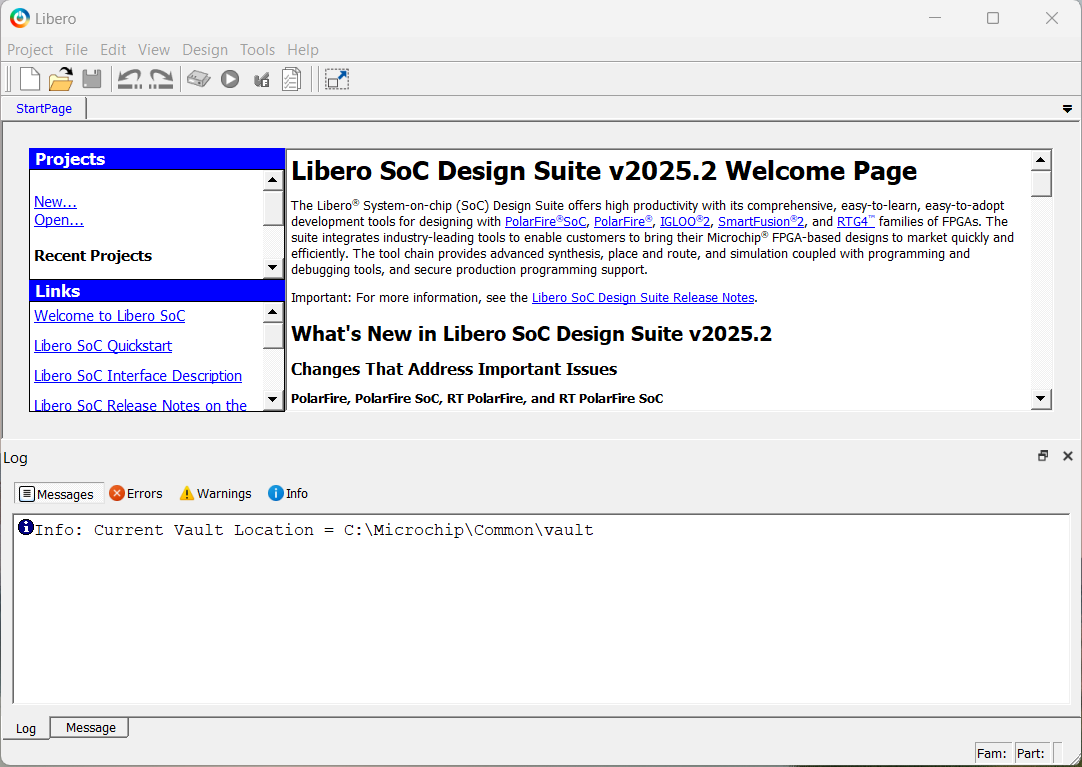
\includegraphics[width=0.85\textwidth]{tutorial_libero_1.png}
    \caption{Página de boas-vindas do Libero SoC Design Suite v2025.2.}
    \label{fig:tut_welcome}
\end{figure}

A partir do menu \textbf{Project $\rightarrow$ Open Project} (ou pelo link 
\textit{Open...} na própria \textit{Welcome Page}), navega-se até a pasta 
raiz do repositório extraído e seleciona-se o arquivo de projeto com 
extensão \texttt{.prjx}, localizado dentro da subpasta 
\texttt{FPGA2memory} (Figura \ref{fig:tut_open}). É esse arquivo que 
referencia toda a estrutura interna do projeto -- pastas \texttt{hdl}, 
\texttt{constraint}, \texttt{synthesis}, \texttt{designer}, entre outras.

\begin{figure}[h!]
    \centering
    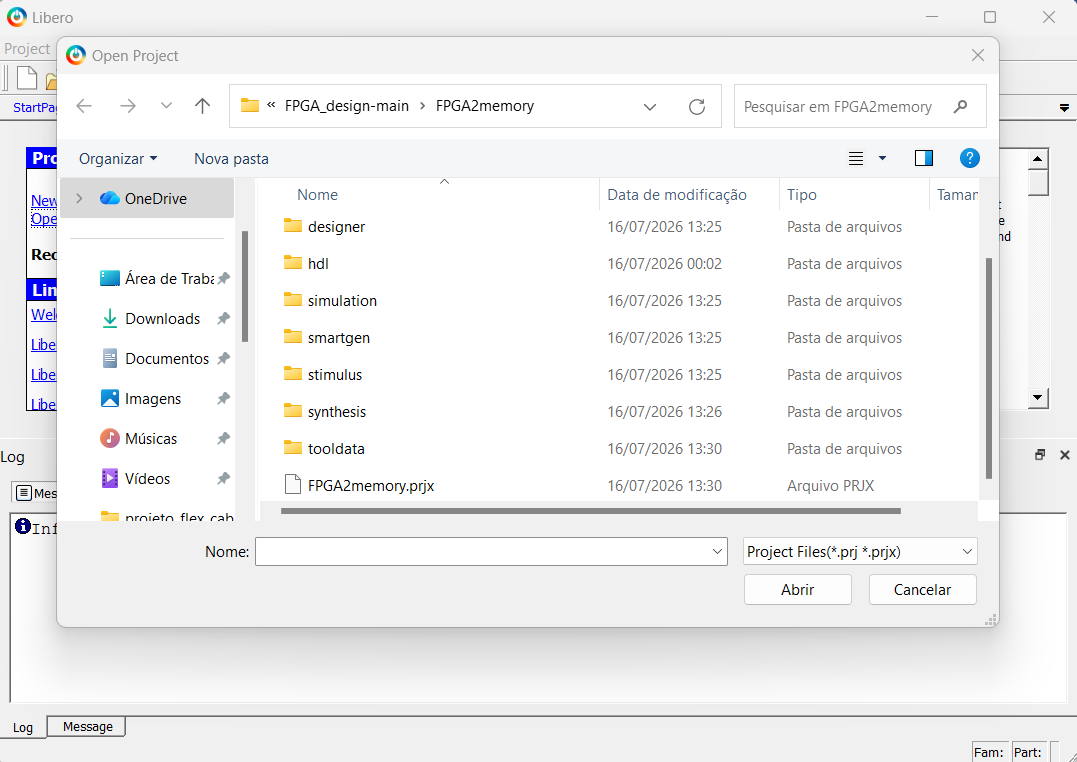
\includegraphics[width=0.85\textwidth]{tutorial_libero_2.png}
    \caption{Seleção do arquivo de projeto \texttt{FPGA2memory.prjx} na janela \textit{Open Project}.}
    \label{fig:tut_open}
\end{figure}

\subsection{Síntese do Design}

Com o projeto aberto, o \textbf{Design Flow} (painel à esquerda) exibe 
todas as etapas do fluxo, da simulação pré-síntese até a gravação final. A 
primeira etapa executada é a \textbf{Synthesize}, que invoca o motor de 
síntese \textit{Synplify Pro} para converter a descrição RTL em 
SystemVerilog (Seção~\ref{sec:arquitetura_hardware}) em uma \textit{netlist} 
de portas lógicas mapeada para a arquitetura da SmartFusion2 (Figura 
\ref{fig:tut_synth_flow}).

\begin{figure}[h!]
    \centering
    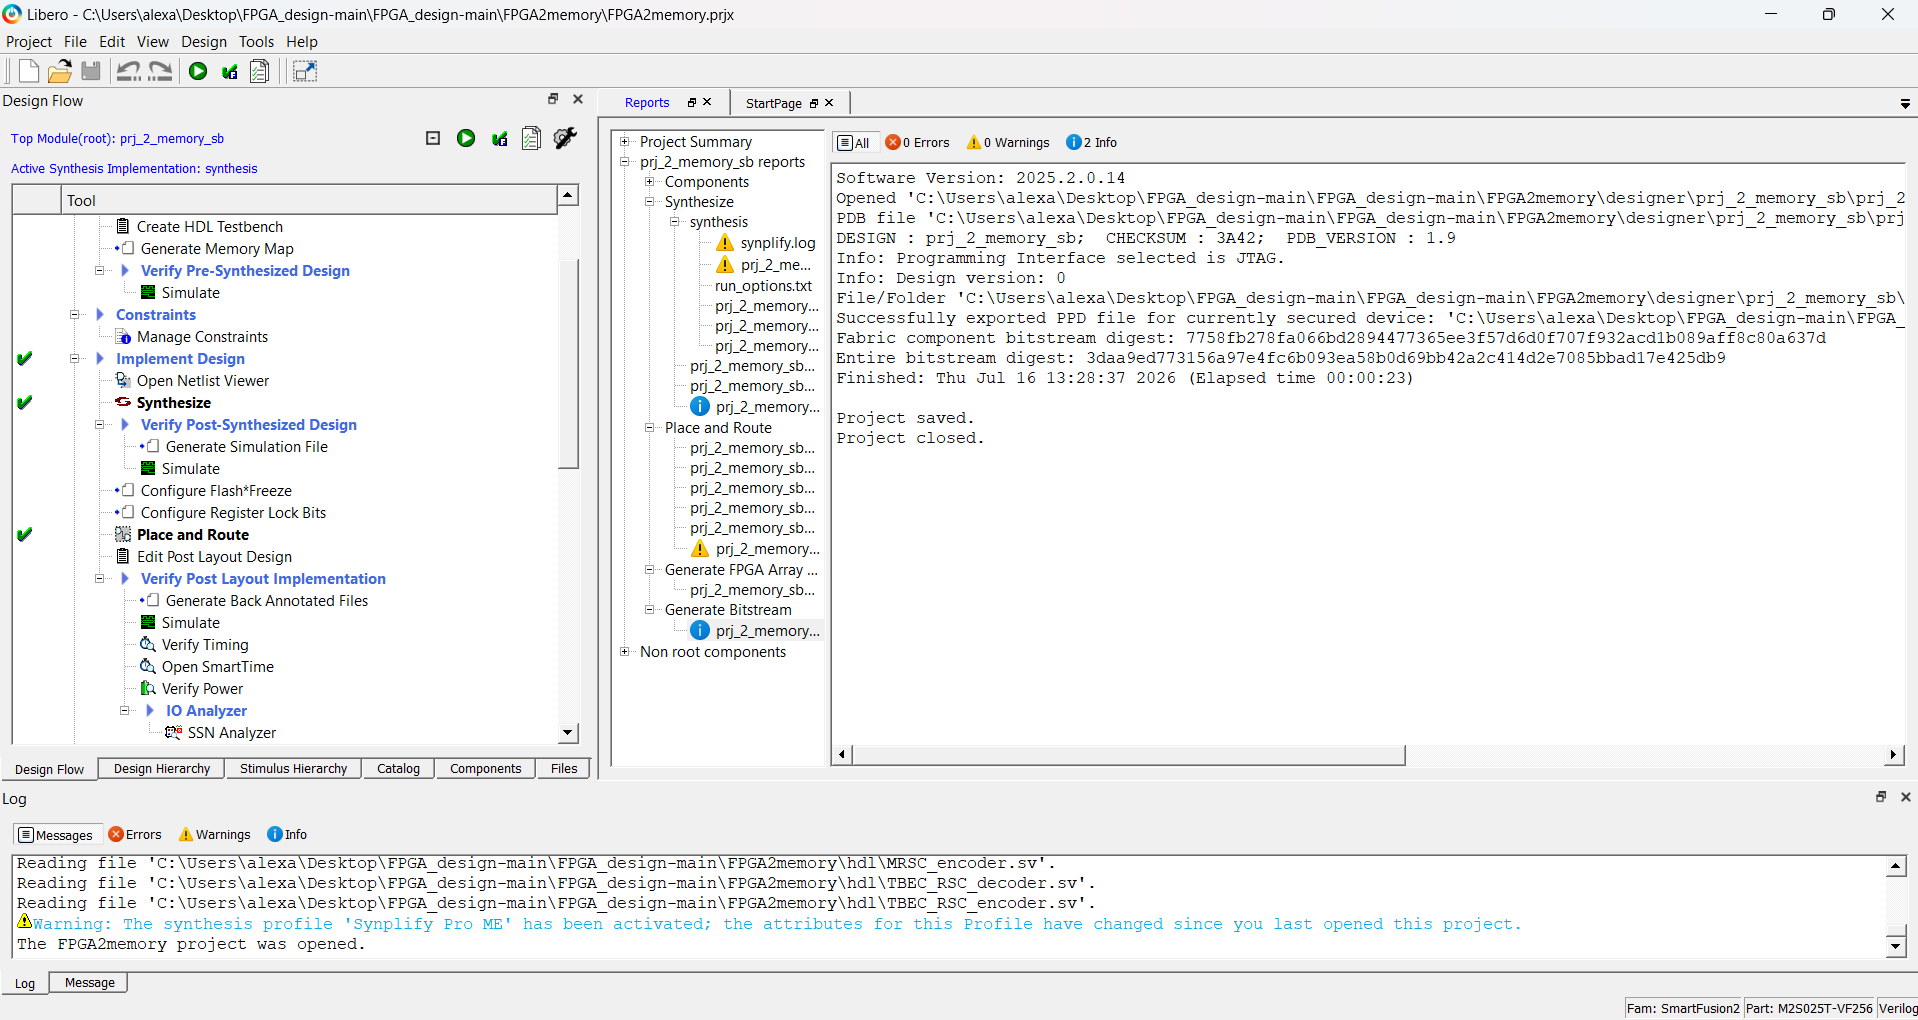
\includegraphics[width=0.85\textwidth]{tutorial_libero_3.png}
    \caption{Árvore do Design Flow durante a leitura dos arquivos-fonte (\texttt{MRSC\_encoder.sv}, \texttt{TBEC\_RSC\_decoder.sv}, etc.) na etapa de síntese.}
    \label{fig:tut_synth_flow}
\end{figure}

O log da ferramenta \textit{Synplify Pro} é exibido em detalhe na aba 
\textbf{Reports}, reportando a versão do sintetizador, o caminho de 
instalação e os argumentos de linha de comando utilizados na chamada 
interna do \texttt{synbatch.exe} (Figura \ref{fig:tut_synplify_log}). Ao 
final dessa etapa, o Libero indica \textit{"Synthesis completed"} no painel 
de mensagens.

\begin{figure}[h!]
    \centering
    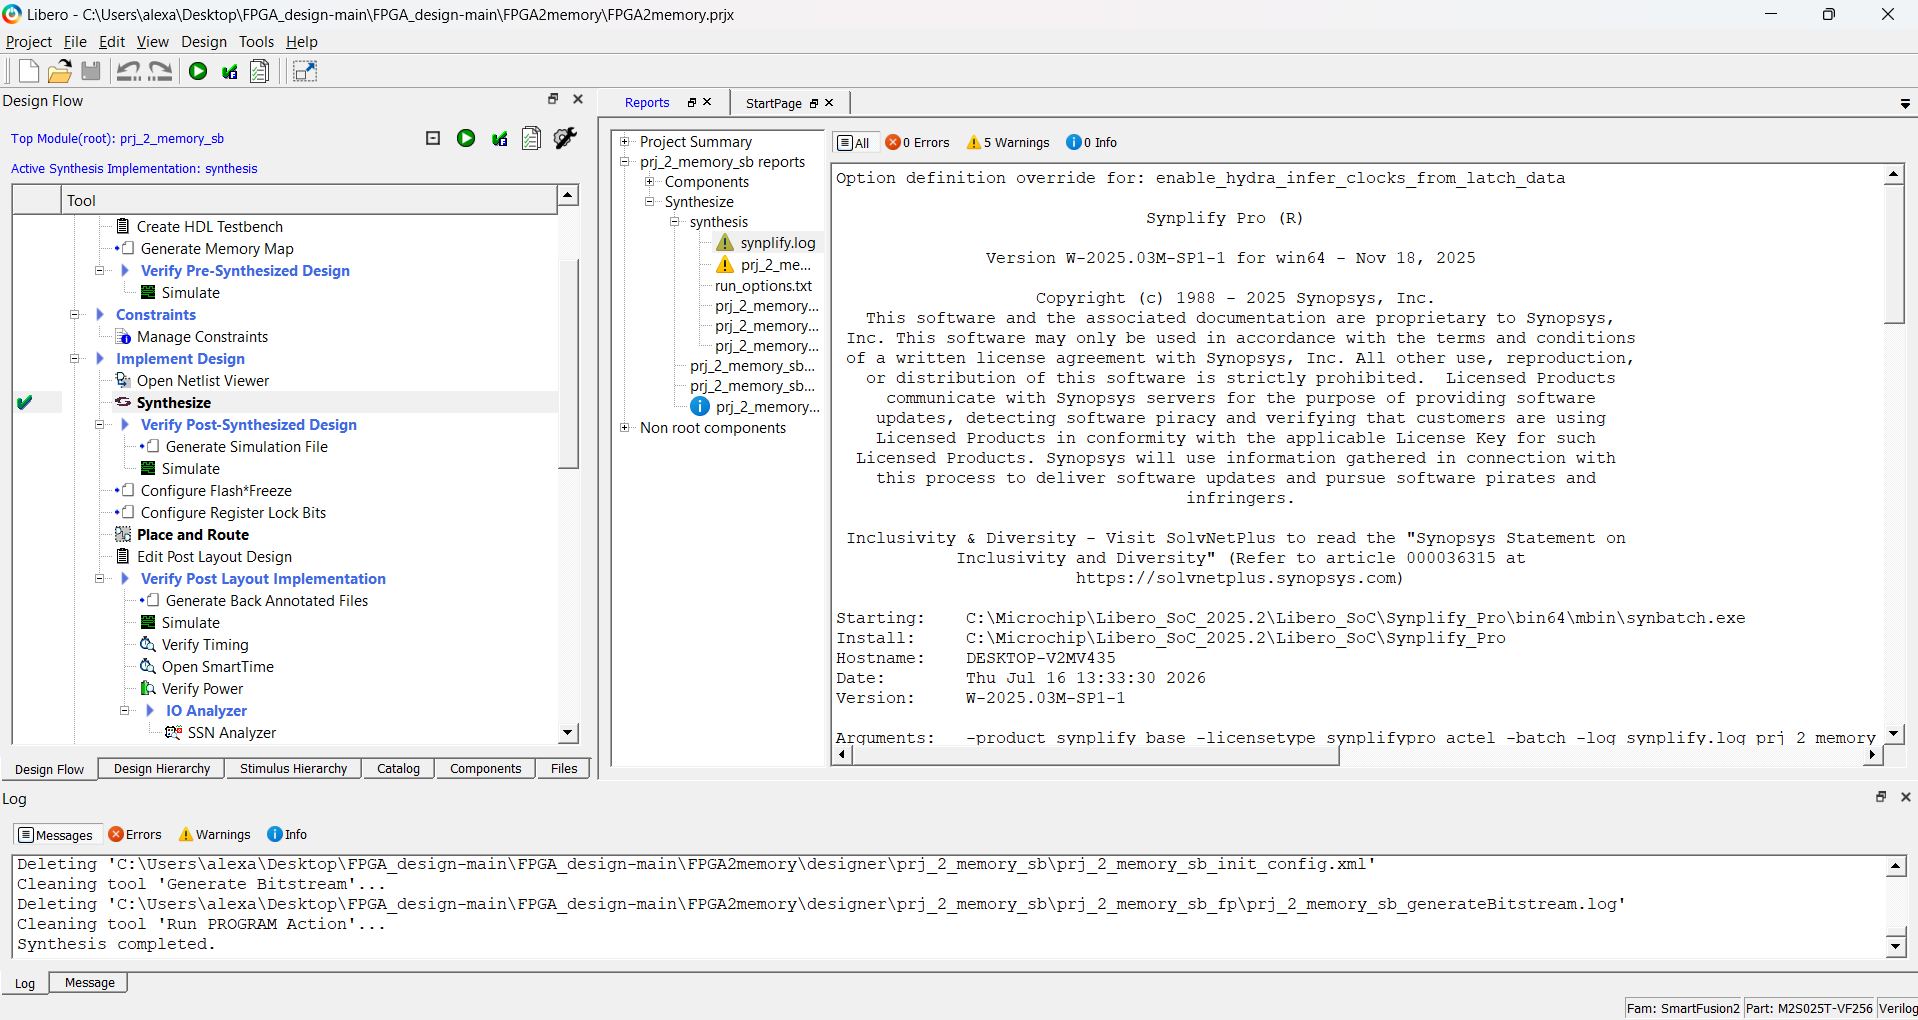
\includegraphics[width=0.85\textwidth]{tutorial_libero_4.png}
    \caption{Log de execução do Synplify Pro (v2025.03M-SP1-1) durante a síntese do projeto.}
    \label{fig:tut_synplify_log}
\end{figure}

\subsection{Place and Route}

Concluída a síntese, a próxima etapa do fluxo é o \textbf{Place and Route}, 
responsável por mapear fisicamente a \textit{netlist} sintetizada nas 
células lógicas, blocos de I/O e recursos de \textit{clock} disponíveis na 
FPGA M2S025T. Ao término dessa etapa, o Libero disponibiliza diversos 
relatórios técnicos -- entre eles o \textbf{Global Net Report}, que detalha 
a alocação das redes de \textit{clock} global (\textit{Global Buffers - 
GB}) e sua taxa de \textit{fanout} (Figura \ref{fig:tut_par_report}).

\begin{figure}[h!]
    \centering
    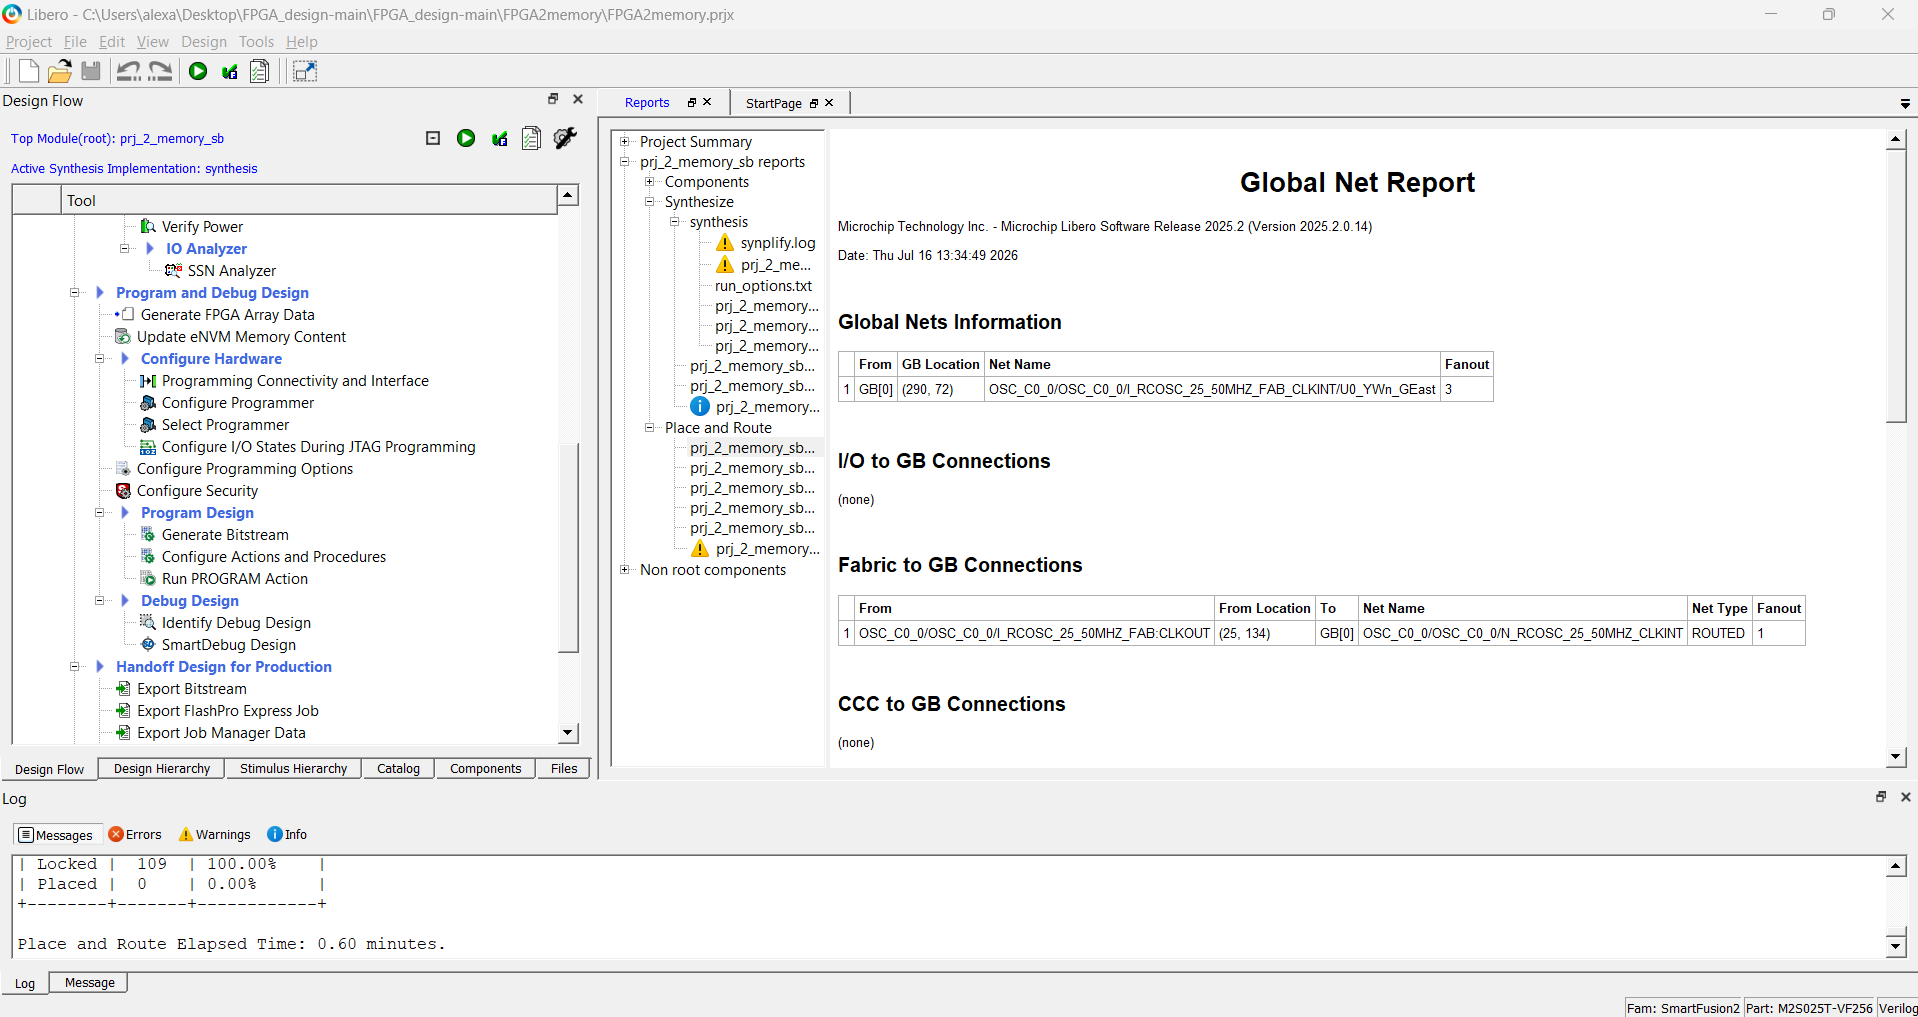
\includegraphics[width=0.85\textwidth]{tutorial_libero_5.png}
    \caption{Relatório de redes globais (\textit{Global Net Report}) gerado após o Place and Route.}
    \label{fig:tut_par_report}
\end{figure}

\subsection{Geração do Bitstream}

Com o \textit{place and route} concluído com sucesso (indicado pelo ícone 
de checagem verde ao lado da etapa na árvore do Design Flow), executa-se a 
etapa \textbf{Generate Bitstream}, dentro da seção \textbf{Program Design}. 
Essa etapa compila o arquivo de configuração binário que será efetivamente 
transferido para a FPGA. O log confirma a finalização do processo com a 
mensagem \textit{"Generating Bitstream File Finished"}, acompanhada dos 
\textit{digests} criptográficos do bitstream gerado, utilizados para 
verificação de integridade (Figura \ref{fig:tut_bitstream}).

\begin{figure}[h!]
    \centering
    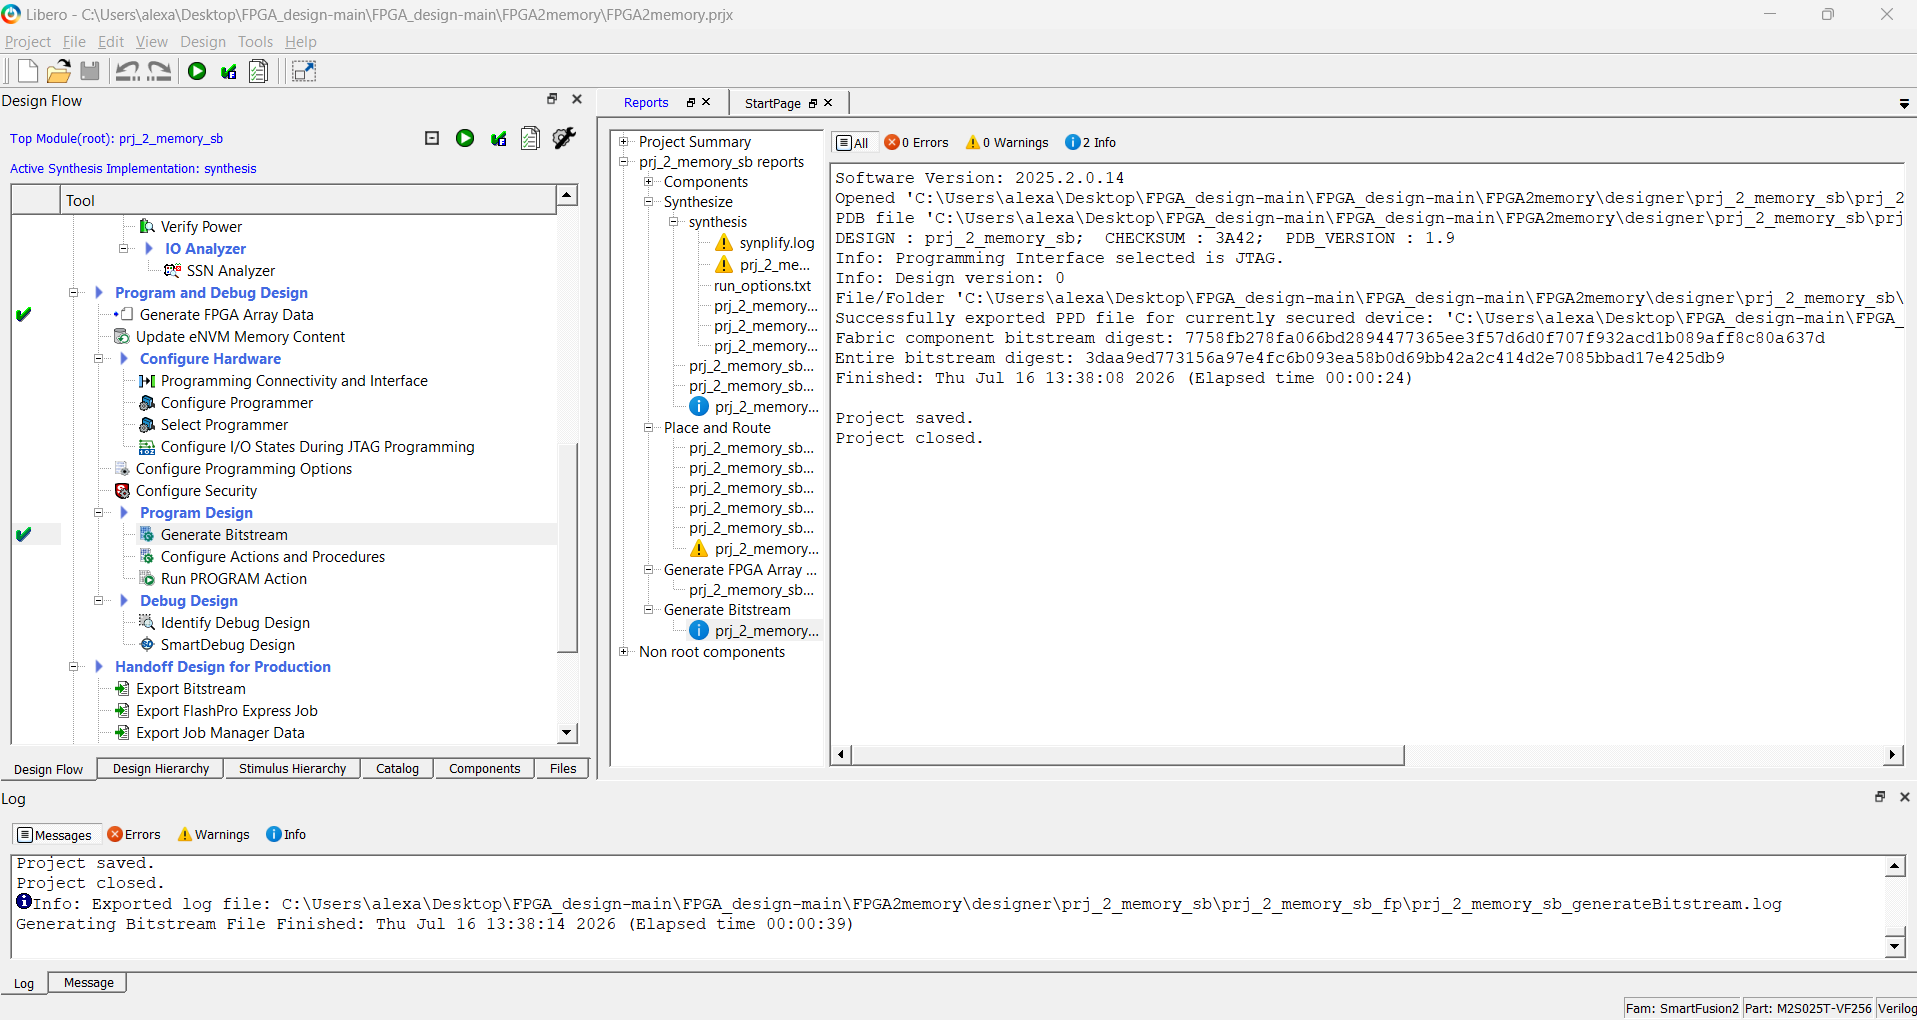
\includegraphics[width=0.85\textwidth]{tutorial_libero_6.png}
    \caption{Conclusão da etapa Generate Bitstream, com os digests do fabric e do bitstream completo.}
    \label{fig:tut_bitstream}
\end{figure}

\subsection{Seleção do Programador (FlashPro) e Gravação}

Com a placa de desenvolvimento conectada ao computador via cabo USB-JTAG 
(programador \textbf{FlashPro5}), acessa-se a etapa \textbf{Select 
Programmer}, dentro de \textbf{Configure Hardware}. O Libero identifica 
automaticamente os programadores conectados fisicamente ao barramento USB, 
exibindo seu identificador de série, o tipo (\texttt{FlashPro5}) e a porta 
de comunicação (Figura \ref{fig:tut_select_prog}). Essa etapa é crítica: o 
identificador do programador salvo no arquivo de projeto deve corresponder 
ao programador fisicamente conectado no momento da gravação -- caso 
contrário, o Libero reporta que o programador esperado não pôde ser 
detectado.

\begin{figure}[h!]
    \centering
    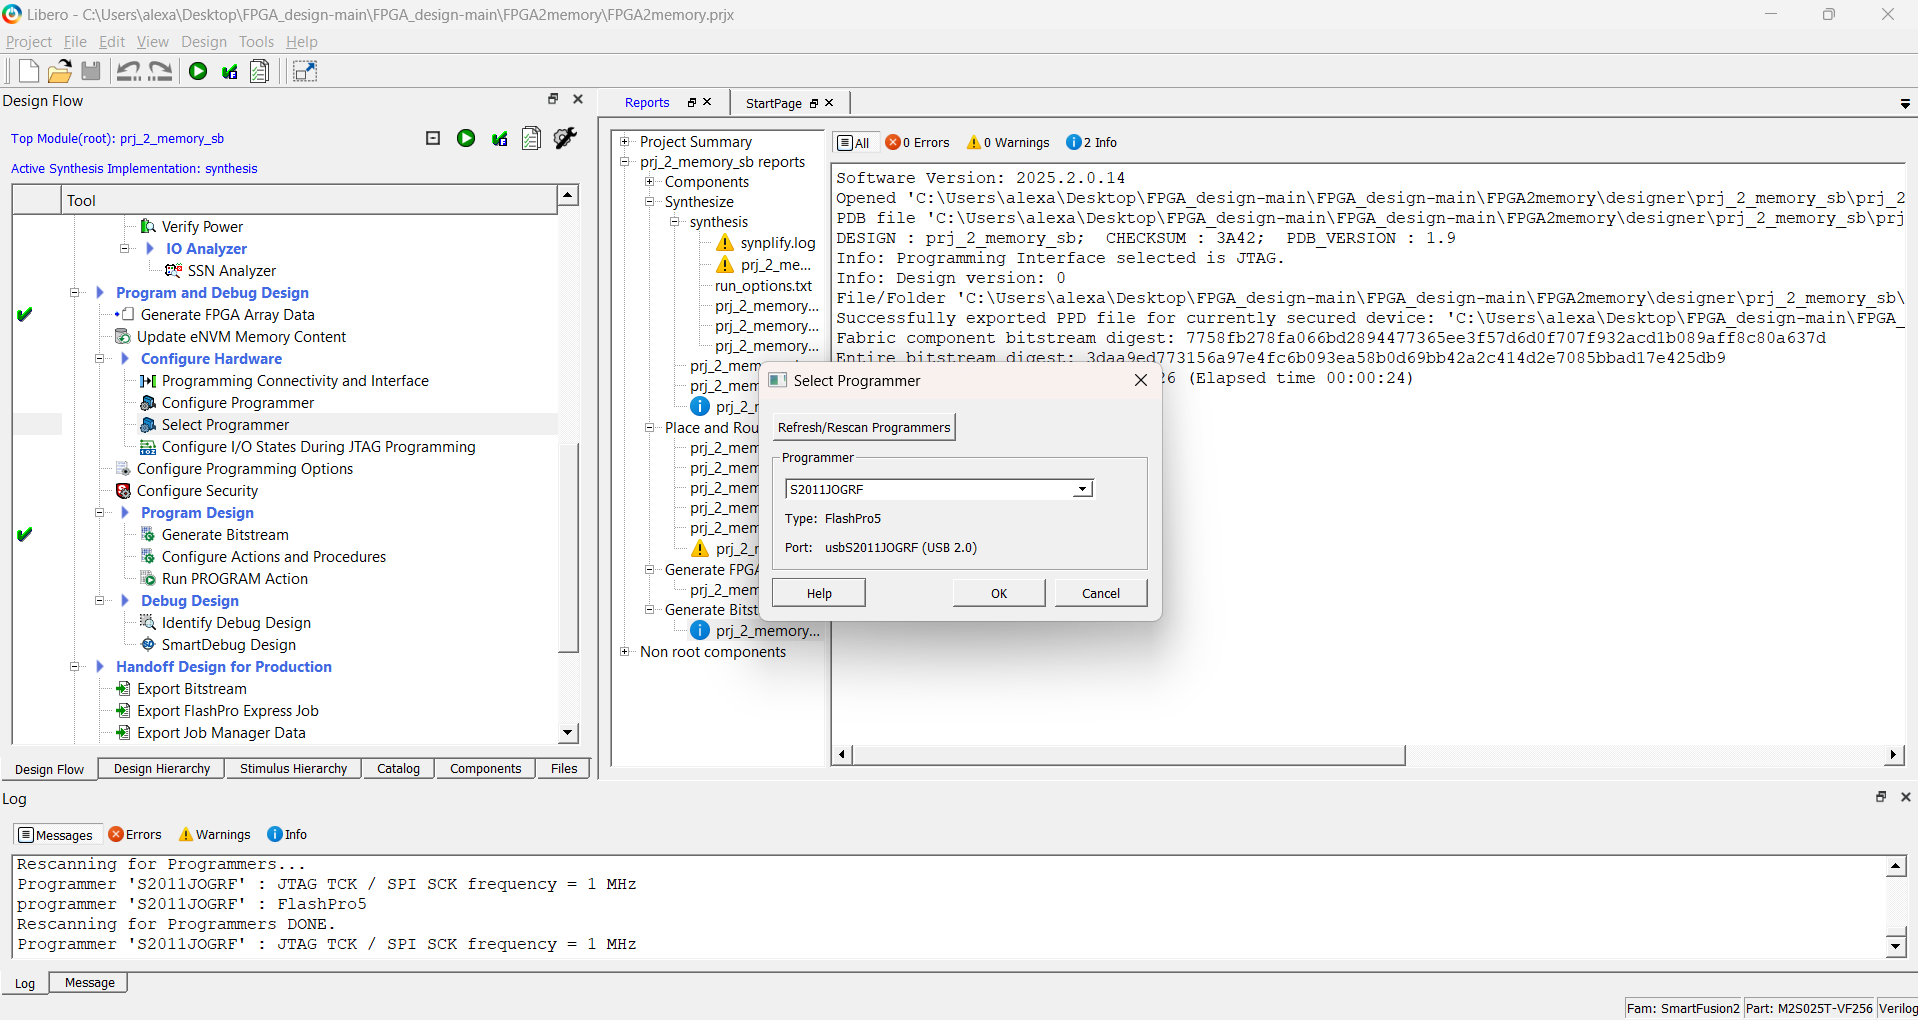
\includegraphics[width=0.85\textwidth]{tutorial_libero_7.png}
    \caption{Janela \textit{Select Programmer} detectando o FlashPro5 conectado (porta USB 2.0).}
    \label{fig:tut_select_prog}
\end{figure}

Após confirmar o programador correto, executa-se a etapa final \textbf{Run 
PROGRAM Action}. O Libero verifica a cadeia JTAG (\textit{Check Chain}), 
confirma que o dispositivo físico corresponde ao \textit{part number} 
configurado no projeto (\texttt{M2S025T-VF256}) e, em caso positivo, 
transfere o bitstream gerado na Seção~\ref{sec:tutorial_libero} para a 
FPGA. Ao final da operação bem-sucedida, o projeto é salvo e fechado 
automaticamente pela ferramenta (Figura \ref{fig:tut_program_done}).

\begin{figure}[h!]
    \centering
    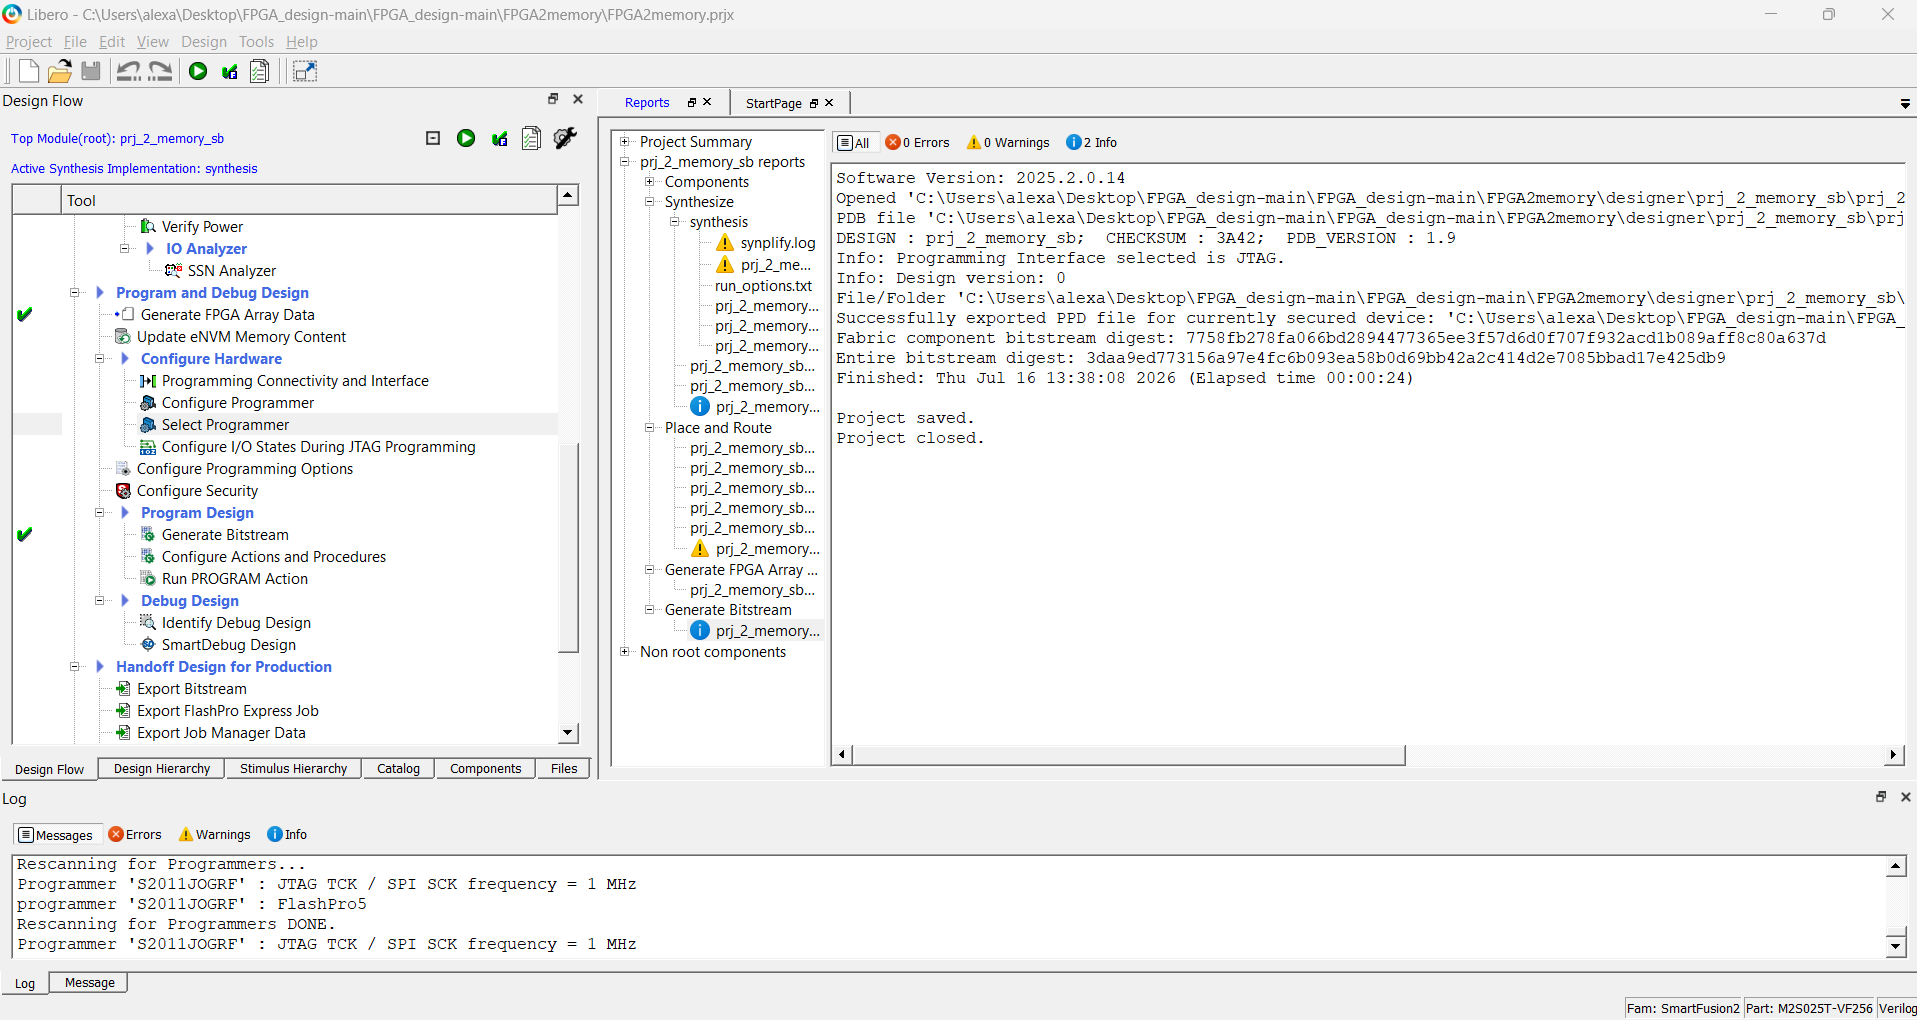
\includegraphics[width=0.85\textwidth]{tutorial_libero_8.png}
    \caption{Conclusão do fluxo de programação: projeto salvo e fechado após a gravação bem-sucedida do bitstream na FPGA.}
    \label{fig:tut_program_done}
\end{figure}

\subsection{Resumo do Fluxo}

Em síntese, o processo completo de gravação segue a sequência: 
(i) abertura do projeto (\texttt{.prjx}); 
(ii) síntese lógica (\textit{Synthesize}); 
(iii) mapeamento físico (\textit{Place and Route}); 
(iv) geração do bitstream (\textit{Generate Bitstream}); 
(v) seleção do programador FlashPro conectado (\textit{Select Programmer}); 
e (vi) gravação efetiva na FPGA (\textit{Run PROGRAM Action}). Uma vez 
concluída essa sequência, o hardware descrito nas 
Seções~\ref{sec:arquitetura_hardware} e~\ref{sec:controle_perifericos} 
passa a operar fisicamente na placa SmartFusion2, pronto para ser validado 
em conjunto com o firmware do STM32 conforme os requisitos de teste da 
Seção~\ref{sec:requisitos_teste}.

% -------------------------------------------------------------------------
% NOVA SUBSEÇÃO: Tutorial de criação de um novo projeto no Libero SoC
% Inserir ANTES de "\subsection{Abertura do Projeto no Libero SoC}"
% dentro de "\section{Tutorial: Gravação do Bitstream na FPGA com o
% Libero SoC 2025.2}" (label sec:tutorial_libero).
%
% As imagens referenciadas devem estar na pasta "imagens/", com os
% nomes originais dos arquivos enviados:
%   imagens/tutorial_projeto_novo_libero_1.png  ...  _16.png
% -------------------------------------------------------------------------

\subsection{Criação de um Novo Projeto no Libero SoC}
\label{sec:tutorial_novo_projeto}

Esta subseção apresenta o fluxo completo para a criação de um projeto
Libero SoC \textbf{do zero}, cobrindo desde a tela de boas-vindas da
ferramenta até a etapa de \textbf{Synthesize} e a atribuição dos pinos
físicos no \textbf{I/O Editor}. A partir do momento em que os pinos
estiverem corretamente atribuídos e comitados, o fluxo se une exatamente
ao tutorial já apresentado na Seção~\ref{sec:tutorial_libero}: o leitor
deve prosseguir diretamente a partir da etapa de \textbf{Place and Route}
(Seção~\ref{sec:tut_par_novo}), repetindo os passos de
\textit{Place and Route}, \textit{Generate Bitstream}, seleção do
programador \textit{FlashPro} e execução do \textit{Run PROGRAM Action}
já descritos anteriormente.

\subsubsection{Página de Boas-Vindas}

Ao iniciar o Libero SoC v2025.2, a ferramenta apresenta a \textit{Welcome
Page}, com atalhos para criar um novo projeto (\textbf{New...}) ou abrir
um projeto existente (\textbf{Open...}), além de projetos recentes e
links de documentação (Figura \ref{fig:novo_welcome}).

\begin{figure}[h!]
    \centering
    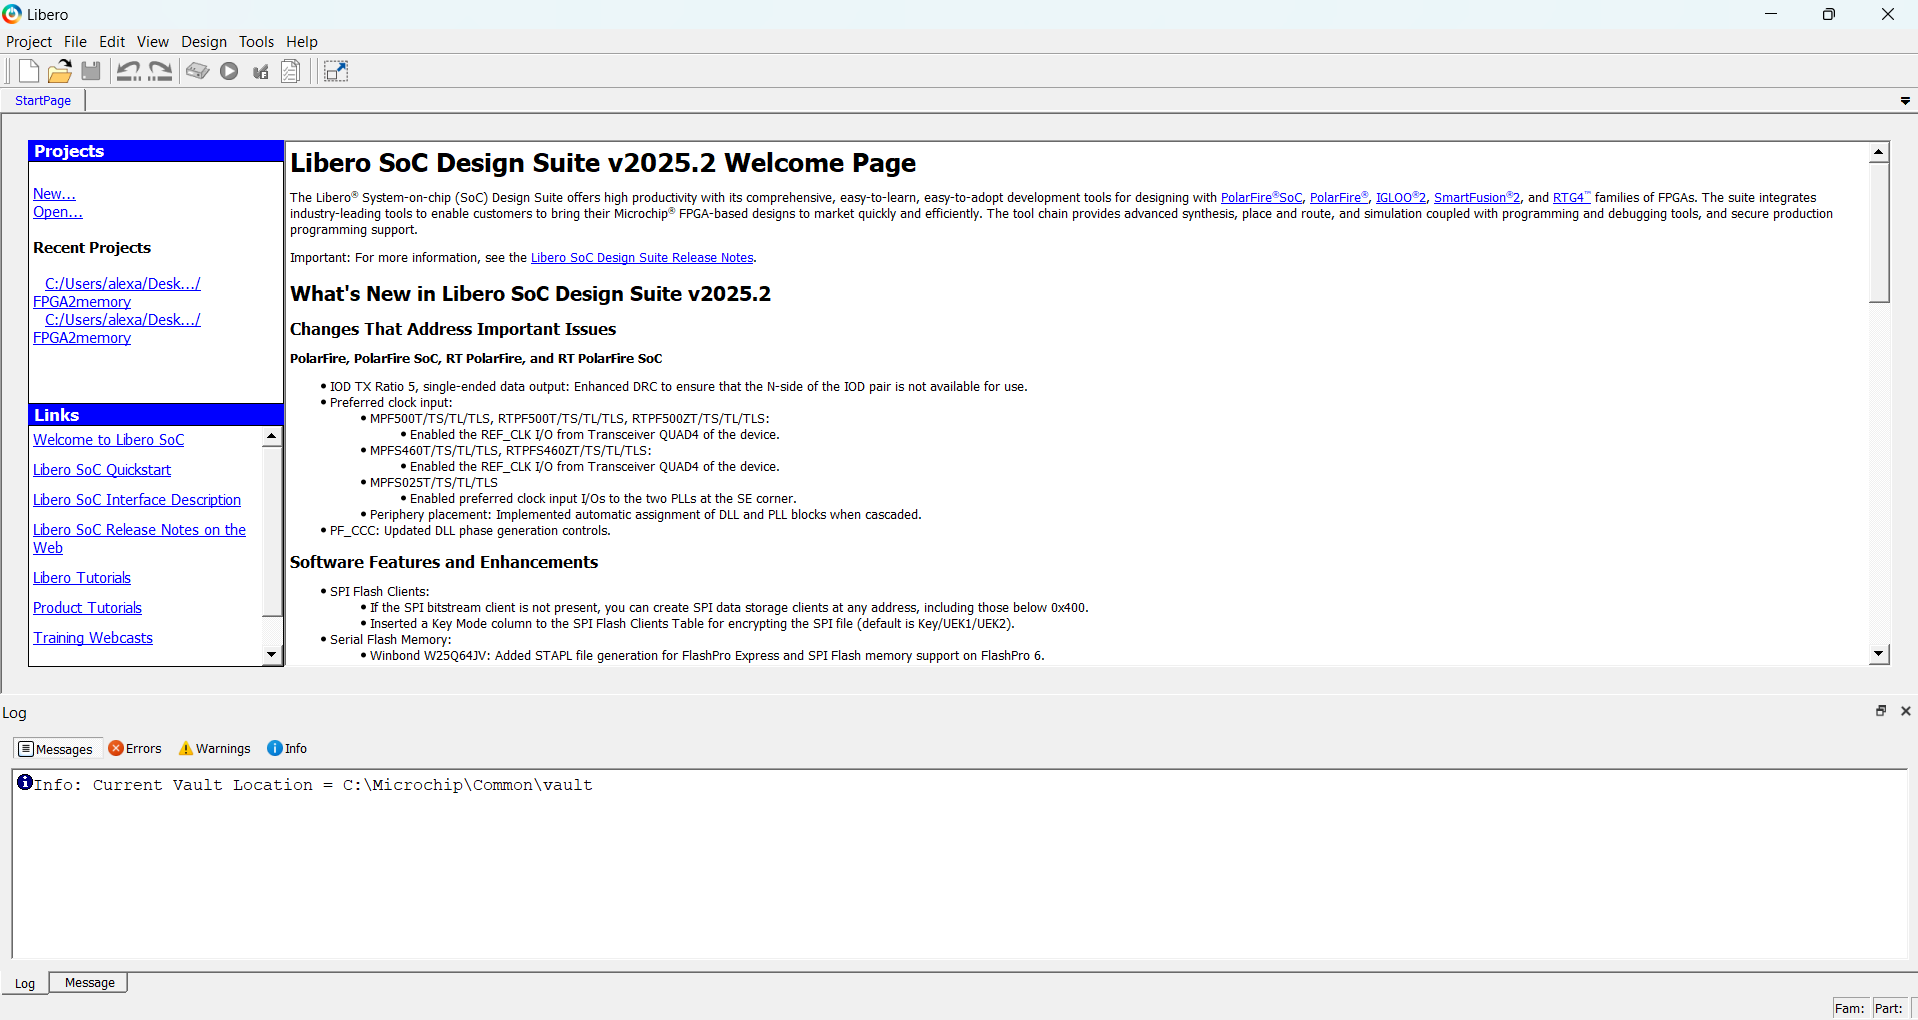
\includegraphics[width=0.85\textwidth]{tutorial_projeto_novo_libero_1.png}
    \caption{Página de boas-vindas do Libero SoC Design Suite v2025.2.}
    \label{fig:novo_welcome}
\end{figure}

\subsubsection{Detalhes do Projeto (\textit{Project Details})}

Ao clicar em \textbf{New...}, o assistente \textit{New project} é aberto
na etapa \textbf{Project Details}. Aqui são definidos o nome do projeto
(\texttt{FPGA\_design}), o diretório onde os arquivos do projeto serão
salvos, e o tipo de HDL preferido (\texttt{Verilog}, que também abrange
arquivos \texttt{.sv} de SystemVerilog). A opção \textbf{Enable block
creation} deve permanecer desmarcada, pois o projeto não será publicado
como um componente reutilizável (Figura \ref{fig:novo_project_details}).

\begin{figure}[h!]
    \centering
    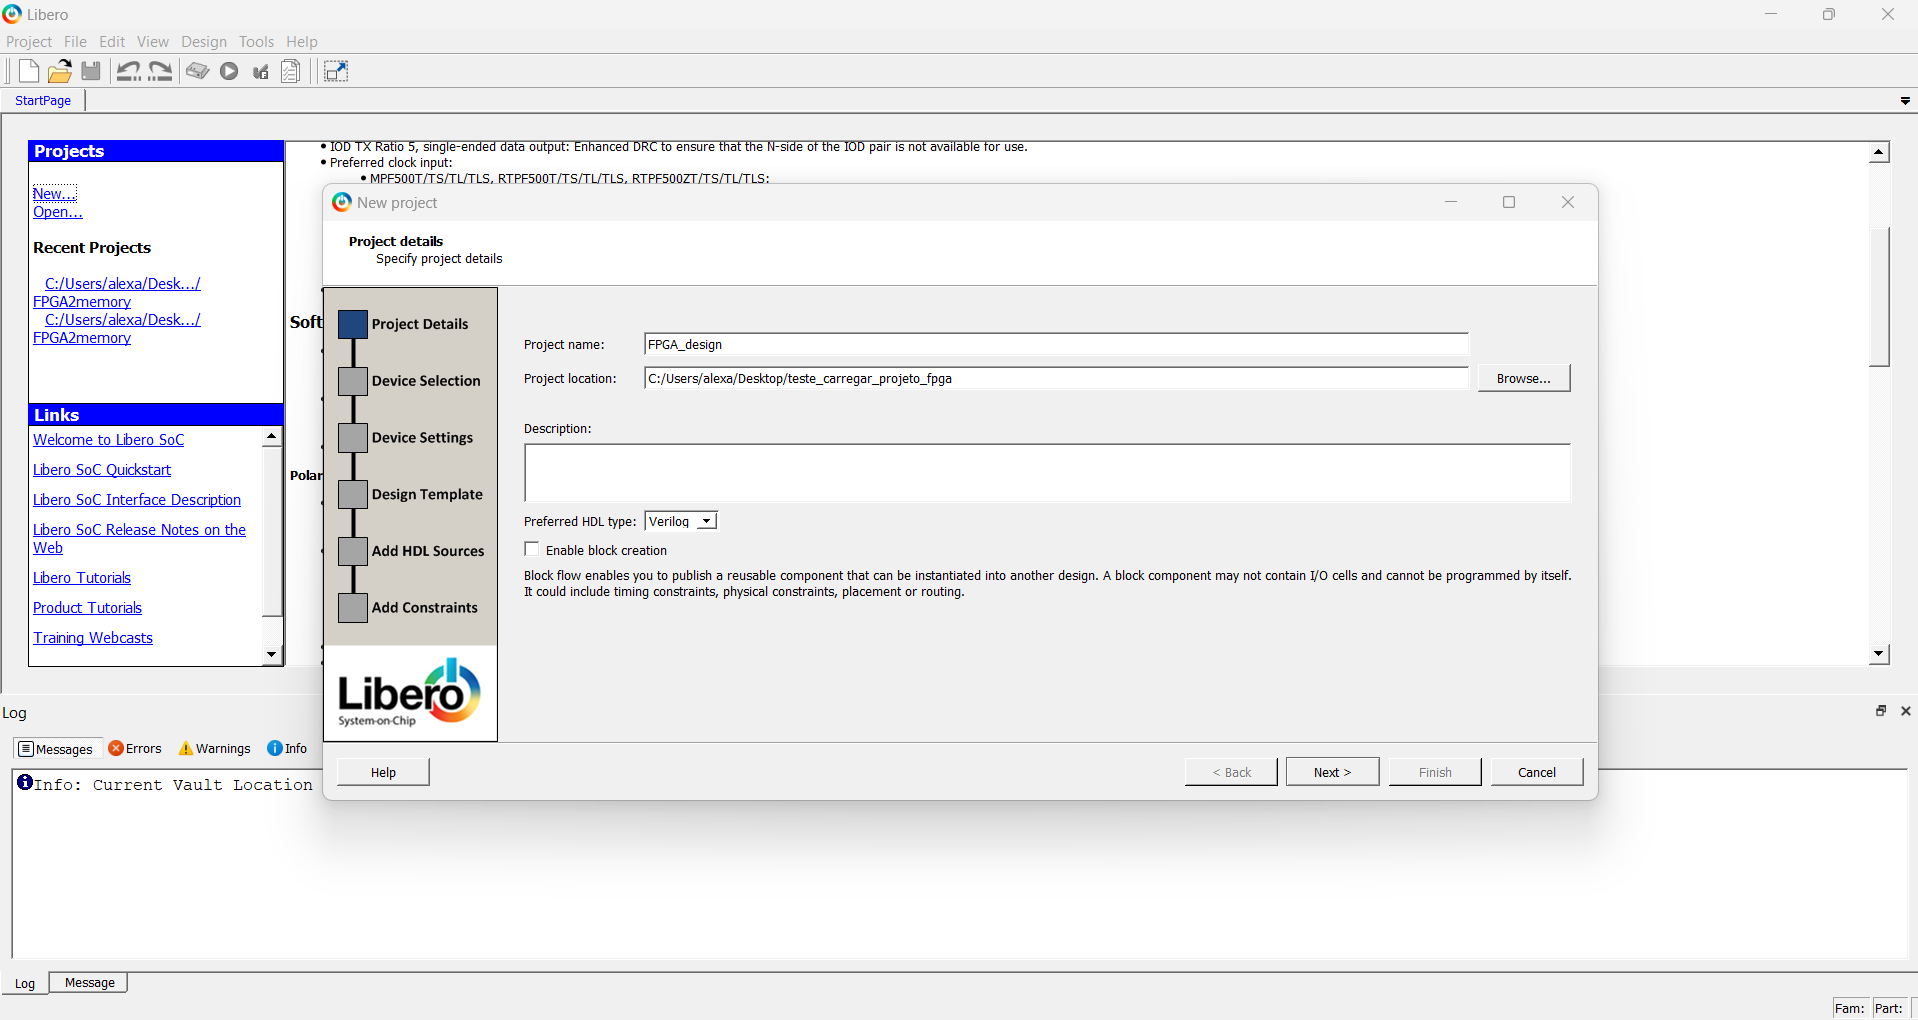
\includegraphics[width=0.85\textwidth]{tutorial_projeto_novo_libero_2.png}
    \caption{Etapa \textit{Project Details} do assistente \textit{New project}.}
    \label{fig:novo_project_details}
\end{figure}

\subsubsection{Seleção do Dispositivo (\textit{Device Selection})}

Na etapa seguinte, filtra-se o dispositivo alvo pela família
\textbf{SmartFusion2}, \textit{die} \textbf{M2S025}, encapsulamento
\textbf{256 VF}, \textit{speed grade} \textbf{STD} e tensão de núcleo
\textbf{1.2}~V. A lista de resultados exibe as duas variantes de
temperatura industrial/comercial disponíveis para esse conjunto de
filtros; seleciona-se o \textit{part number}
\textbf{M2S025-VF256I}, correspondente ao dispositivo efetivamente
utilizado na placa NASCERR (Figura \ref{fig:novo_device_selection}).

\begin{figure}[h!]
    \centering
    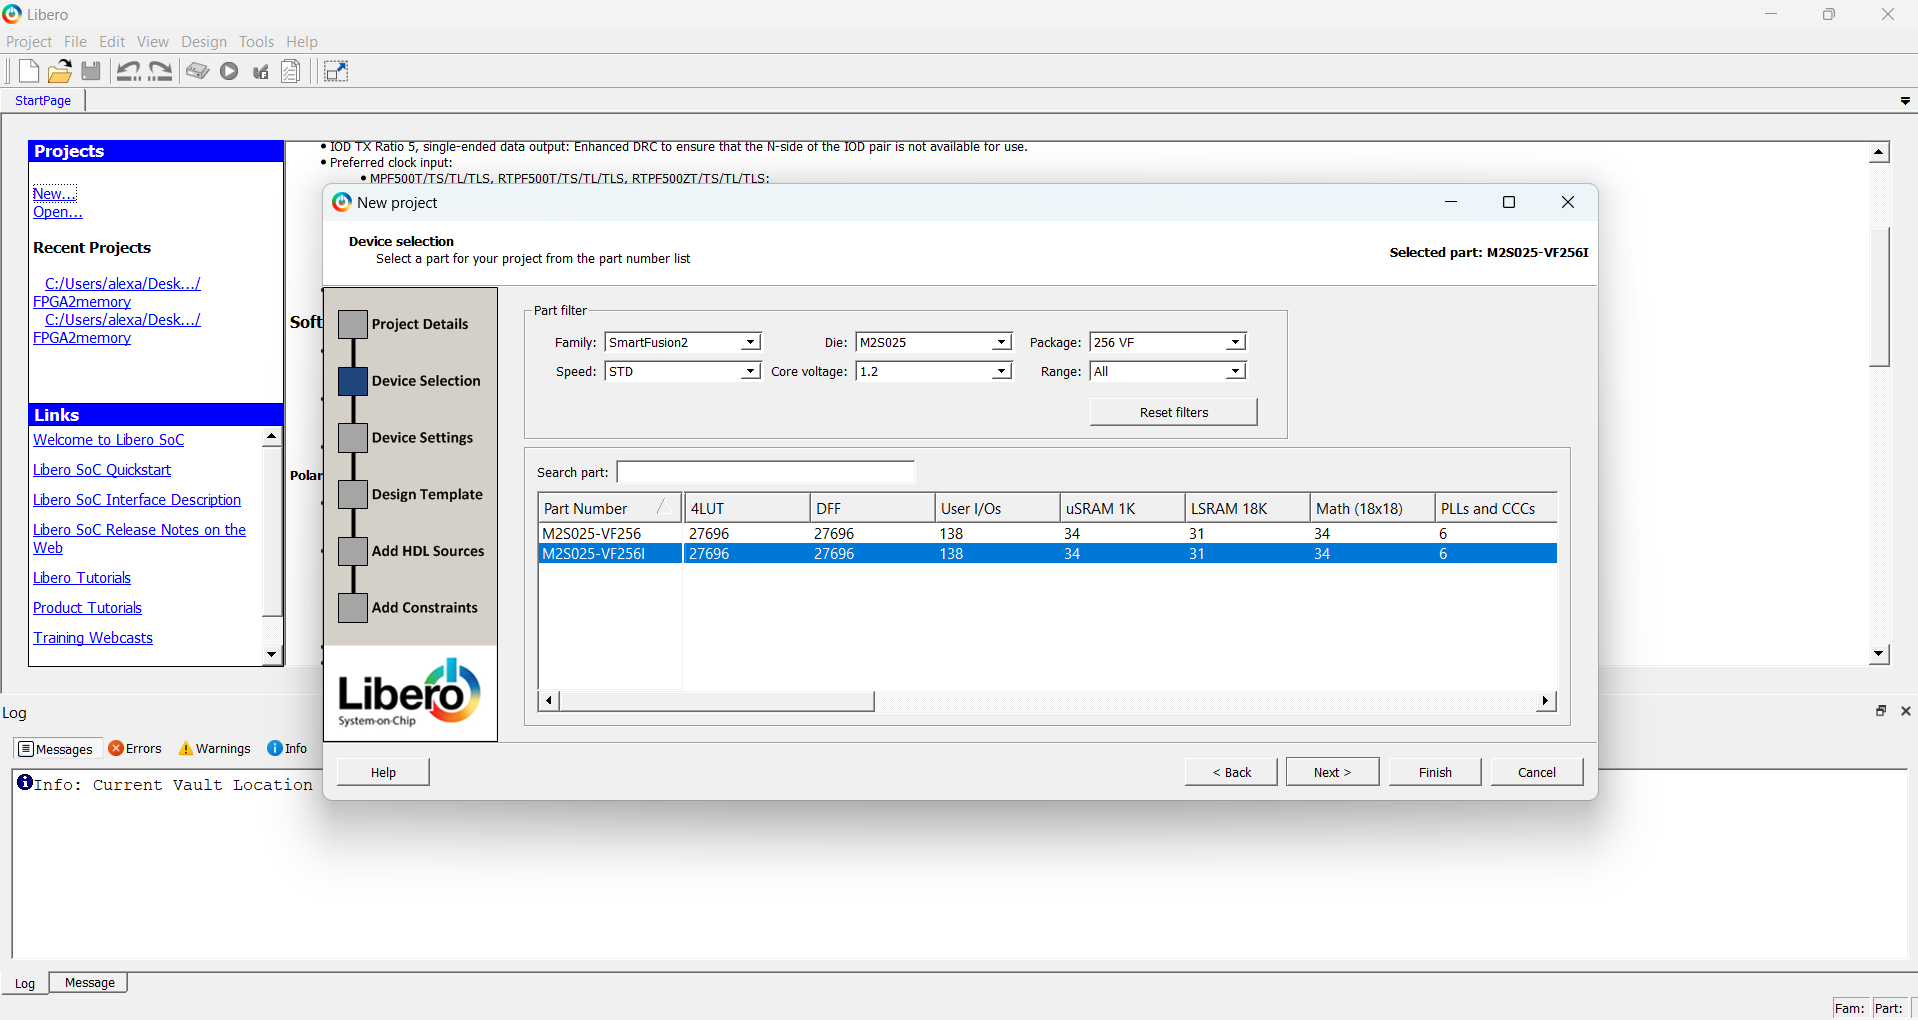
\includegraphics[width=0.85\textwidth]{tutorial_projeto_novo_libero_3.png}
    \caption{Etapa \textit{Device Selection}, com os filtros de família, \textit{die}, encapsulamento e tensão aplicados.}
    \label{fig:novo_device_selection}
\end{figure}

\subsubsection{Configurações do Dispositivo (\textit{Device Settings})}

Nesta etapa, define-se a tecnologia de I/O padrão como
\textbf{LVCMOS 2.5V} (compatível com a tensão de alimentação dos bancos
de I/O utilizados pelos barramentos de dados do projeto) e mantém-se a
opção \textbf{Reserve pins for probes} habilitada. Nas configurações de
alimentação, a tensão de \textit{PLL supply} é mantida em \textbf{2.5}~V
e o tempo de \textit{ramp} da alimentação em \textbf{100ms} (Figura
\ref{fig:novo_device_settings}).

\begin{figure}[h!]
    \centering
    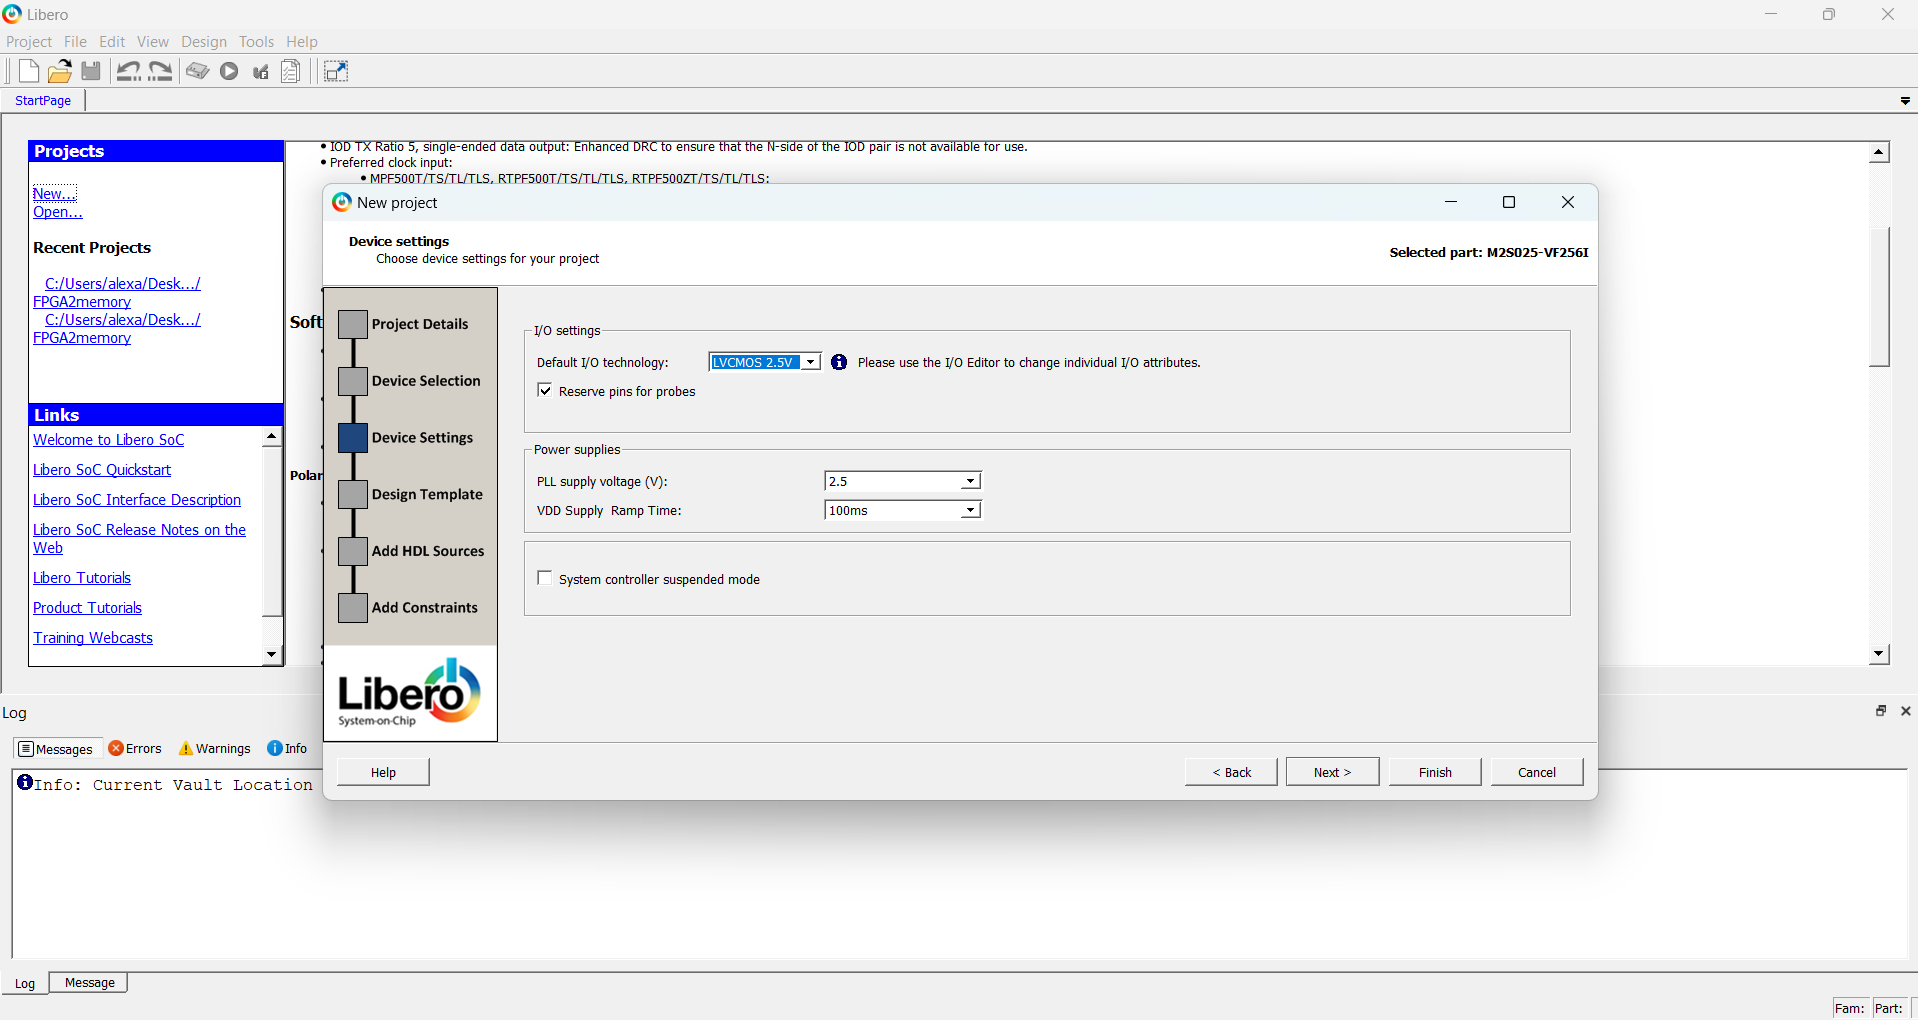
\includegraphics[width=0.85\textwidth]{tutorial_projeto_novo_libero_4.png}
    \caption{Etapa \textit{Device Settings}: tecnologia de I/O e alimentação.}
    \label{fig:novo_device_settings}
\end{figure}

\subsubsection{Modelo de Design (\textit{Design Template})}

Na etapa \textbf{Design Template}, seleciona-se a opção \textbf{None}.
Diferentemente de projetos que utilizam o \textit{System Builder} para
instanciar o Microcontroller Subsystem (MSS) da SmartFusion2, o módulo
\texttt{fpga\_top\_design} (Seção~\ref{sec:nivel3_toplevel}) opera
inteiramente na \textit{fabric} da FPGA, sem qualquer dependência do
Cortex-M interno ou de periféricos do MSS -- a comunicação com o
processador STM32 externo ocorre diretamente pelos pinos de
\textit{fabric} descritos na Seção~\ref{sec:controle_perifericos}. Por
esse motivo, nenhum dos modelos baseados em \textit{System Builder} ou em
MSS é necessário (Figura \ref{fig:novo_design_template}).

\begin{figure}[h!]
    \centering
    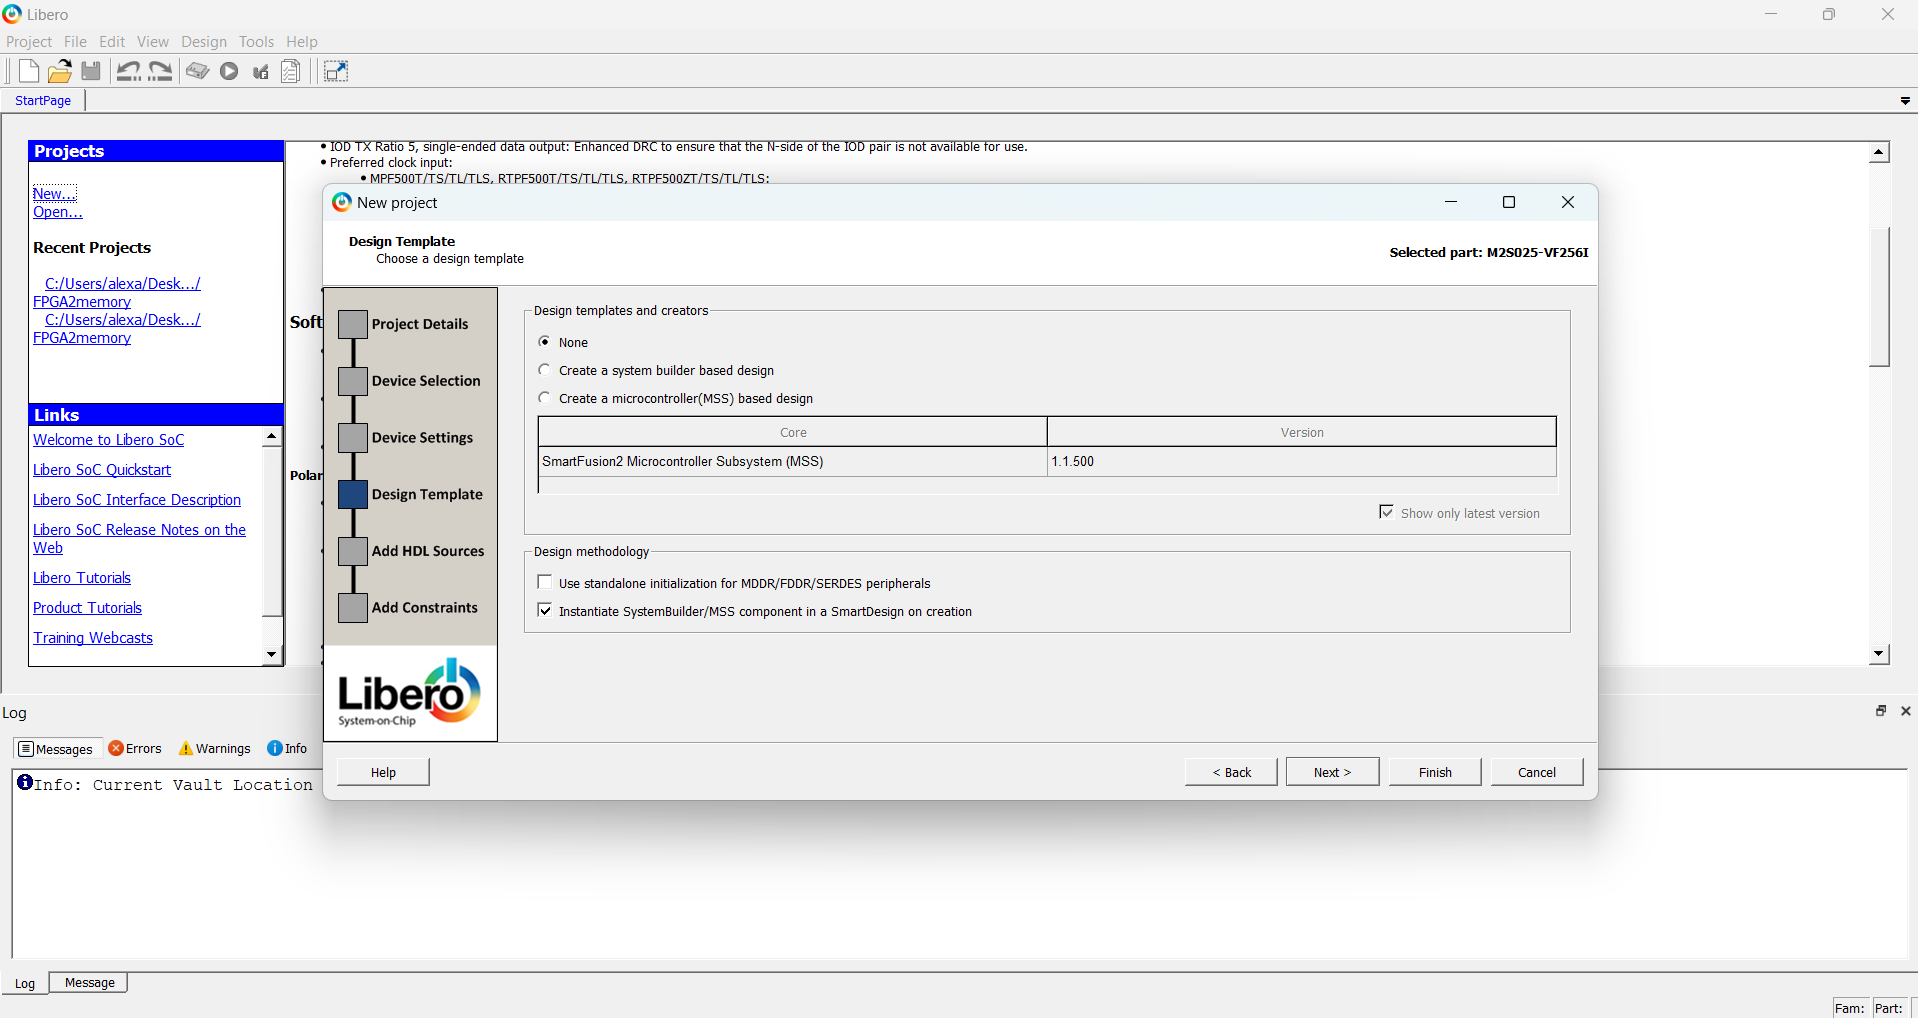
\includegraphics[width=0.85\textwidth]{tutorial_projeto_novo_libero_5.png}
    \caption{Etapa \textit{Design Template} com a opção \textbf{None} selecionada.}
    \label{fig:novo_design_template}
\end{figure}

\subsubsection{Importação dos Arquivos-Fonte (\textit{Add HDL Sources})}

A etapa \textbf{Add HDL Sources} é inicialmente exibida vazia (Figura
\ref{fig:novo_hdl_vazio}). Por meio do botão \textbf{Import file}, são
selecionados os seis arquivos SystemVerilog que compõem a hierarquia
completa do projeto (Seção~\ref{sec:arquitetura_hardware}):
\texttt{design.sv} (Nível 3, top-level), \texttt{ecc\_design.sv} (Nível
2, multiplexador de ECC), e os quatro codecs de Nível 1:
\texttt{MRSC\_encoder.sv}, \texttt{MRSC\_decoder.sv},
\texttt{TBEC\_RSC\_encoder.sv} e \texttt{TBEC\_RSC\_decoder.sv} (Figura
\ref{fig:novo_hdl_import}). Após a importação, cada arquivo aparece
listado com o status \textbf{Imported} e o caminho de origem
correspondente (Figura \ref{fig:novo_hdl_importado}).

\begin{figure}[h!]
    \centering
    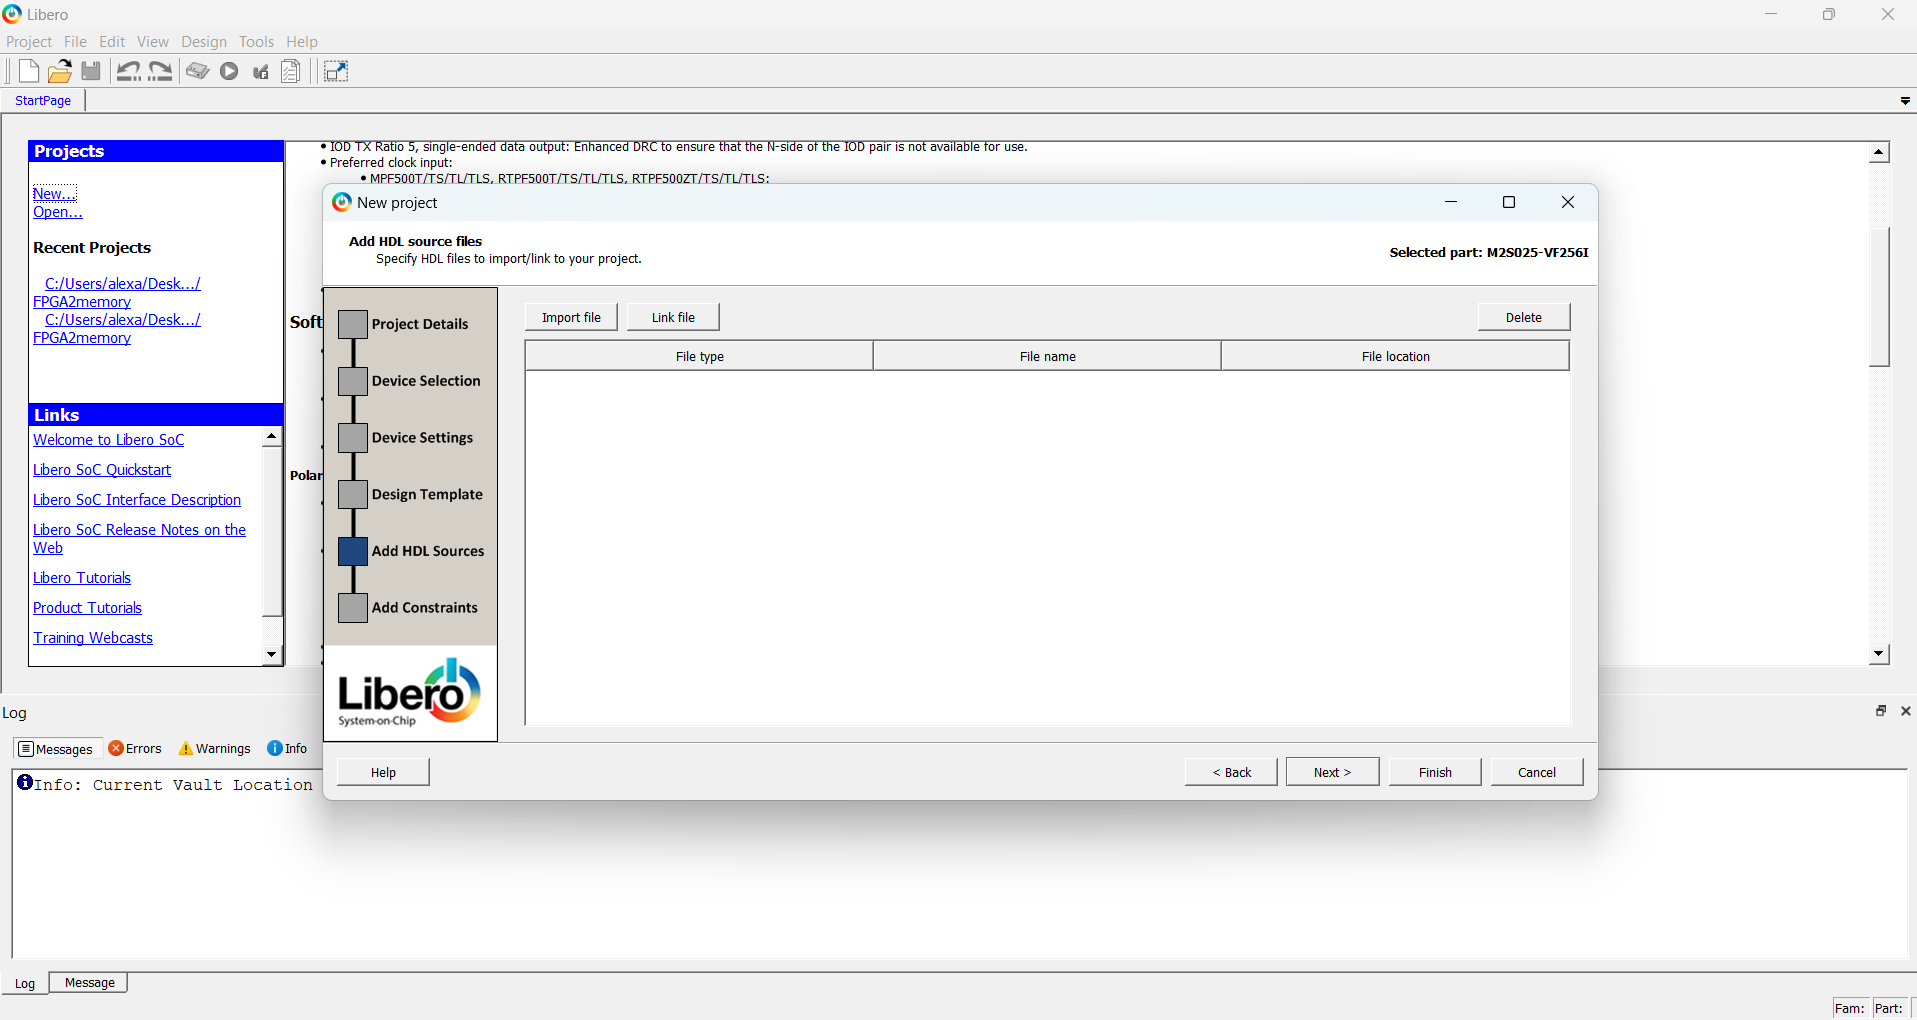
\includegraphics[width=0.85\textwidth]{tutorial_projeto_novo_libero_6.png}
    \caption{Etapa \textit{Add HDL Sources} antes da importação dos arquivos.}
    \label{fig:novo_hdl_vazio}
\end{figure}

\begin{figure}[h!]
    \centering
    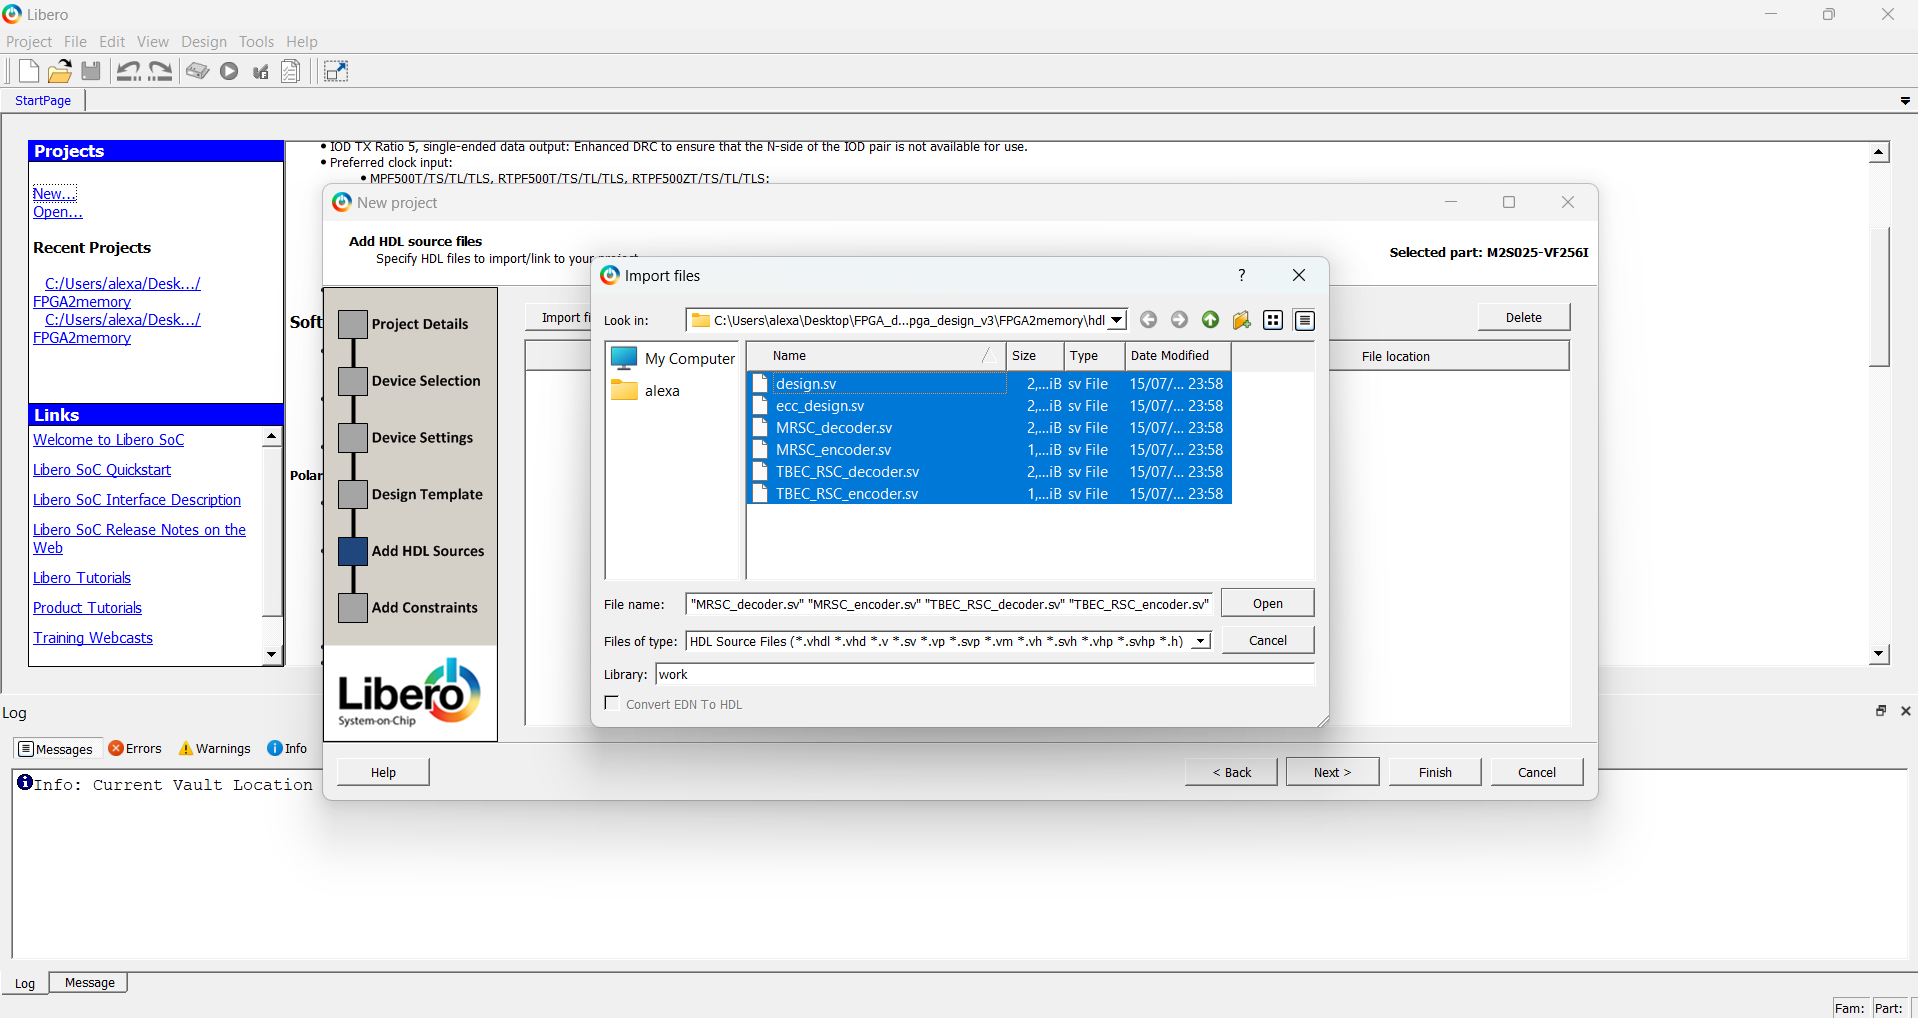
\includegraphics[width=0.85\textwidth]{tutorial_projeto_novo_libero_7.png}
    \caption{Janela \textit{Import files} com os seis arquivos \texttt{.sv} do projeto selecionados.}
    \label{fig:novo_hdl_import}
\end{figure}

\begin{figure}[h!]
    \centering
    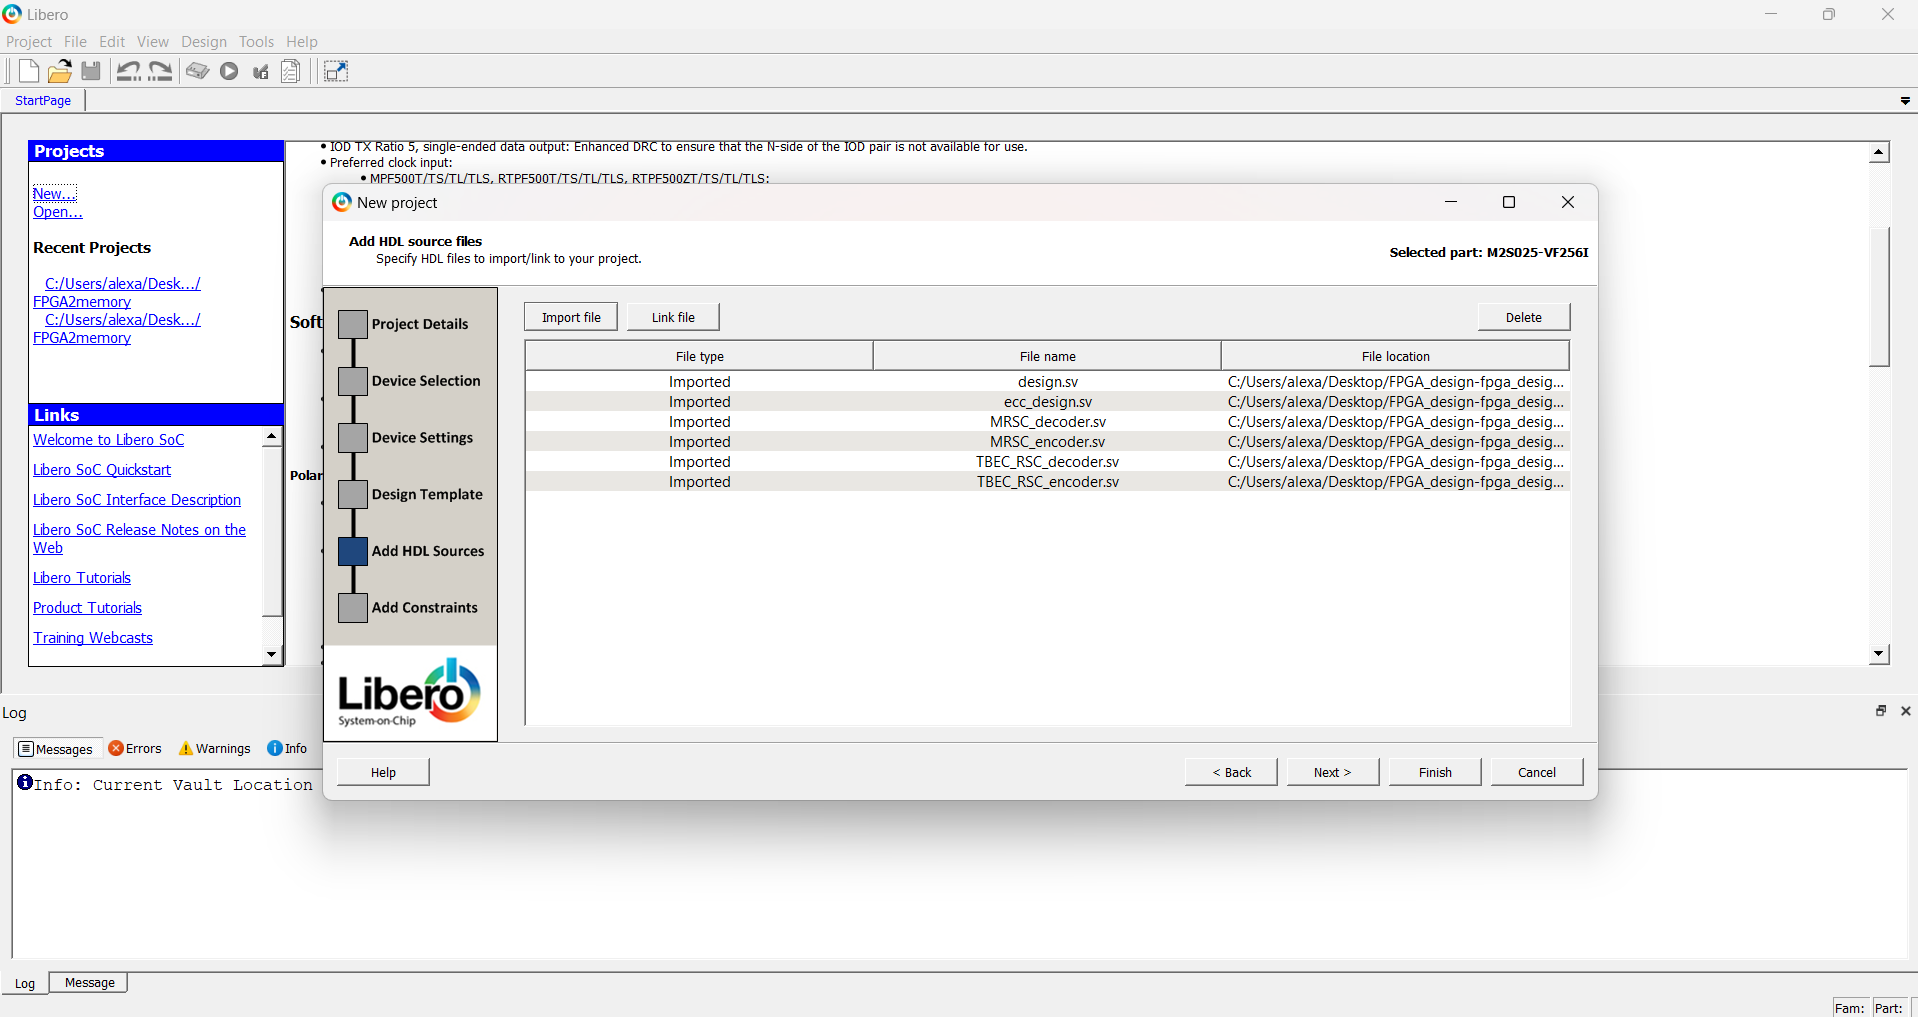
\includegraphics[width=0.85\textwidth]{tutorial_projeto_novo_libero_8.png}
    \caption{Arquivos-fonte importados com sucesso para o projeto.}
    \label{fig:novo_hdl_importado}
\end{figure}

Ao clicar em \textbf{Finish}, o projeto é criado e a mensagem
\textit{"The FPGA\_design project was created"} é exibida no painel de
\textbf{Log} (Figura \ref{fig:novo_criado}). Nesse momento, o painel
\textbf{Design Hierarchy} exibe um aviso amarelo \textit{"Please select a
root"}, indicando que, embora os arquivos já estejam associados ao
projeto, o módulo de topo ainda não foi identificado.

\begin{figure}[h!]
    \centering
    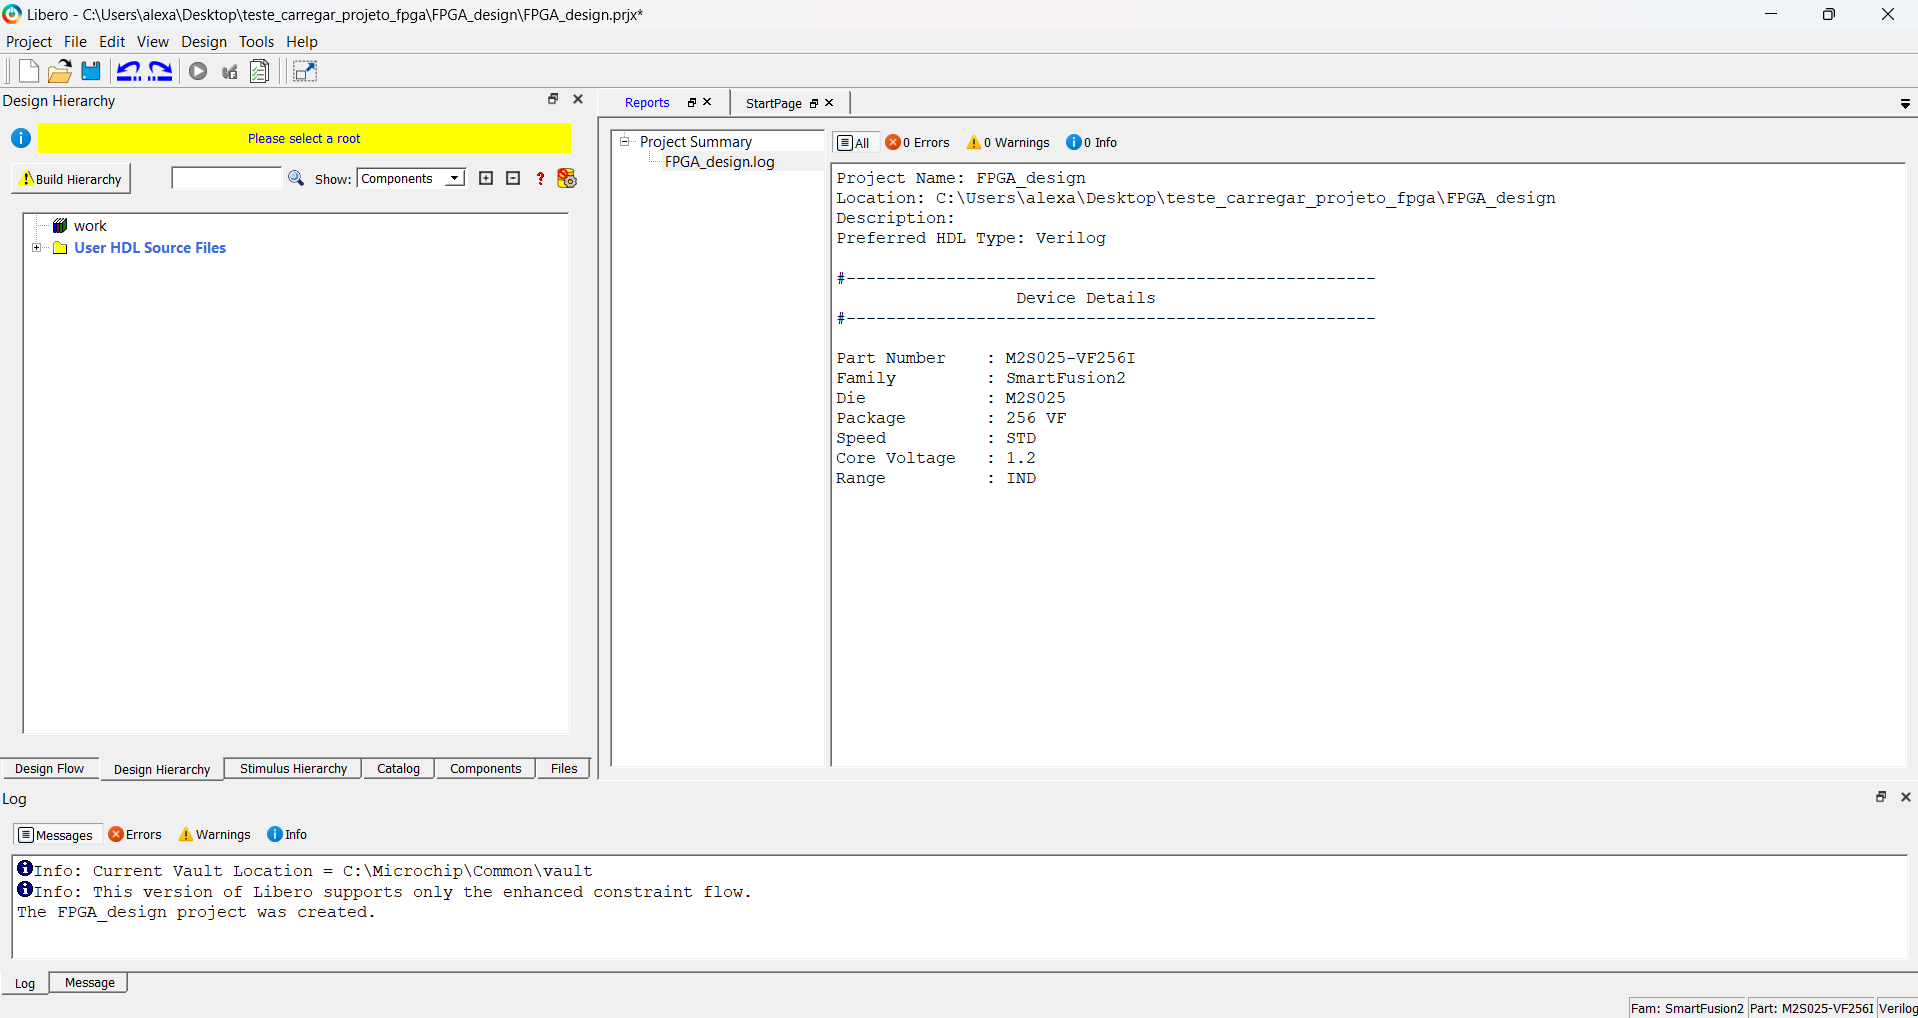
\includegraphics[width=0.85\textwidth]{tutorial_projeto_novo_libero_9.png}
    \caption{Projeto \texttt{FPGA\_design} recém-criado, com o aviso \textit{"Please select a root"}.}
    \label{fig:novo_criado}
\end{figure}

\subsubsection{Definição do Módulo de Topo (\textit{Set As Root})}

Após acionar o botão \textbf{Build Hierarchy}, o Libero interpreta os
arquivos-fonte e identifica os módulos SystemVerilog neles declarados,
listando o módulo \texttt{fpga\_top\_design} (definido no arquivo
\texttt{design.sv}) na raiz da árvore \texttt{work}. Clicando com o botão
direito sobre esse módulo, seleciona-se a opção \textbf{Set As Root} no
menu de contexto, definindo-o formalmente como o módulo de topo (Figura
\ref{fig:novo_set_root}). O painel de \textbf{Log} confirma a leitura de
todos os arquivos da hierarquia (\texttt{ecc\_design.sv},
\texttt{MRSC\_decoder.sv}, \texttt{MRSC\_encoder.sv},
\texttt{TBEC\_RSC\_decoder.sv} e \texttt{TBEC\_RSC\_encoder.sv}), sem a
ocorrência de erros.

\begin{figure}[h!]
    \centering
    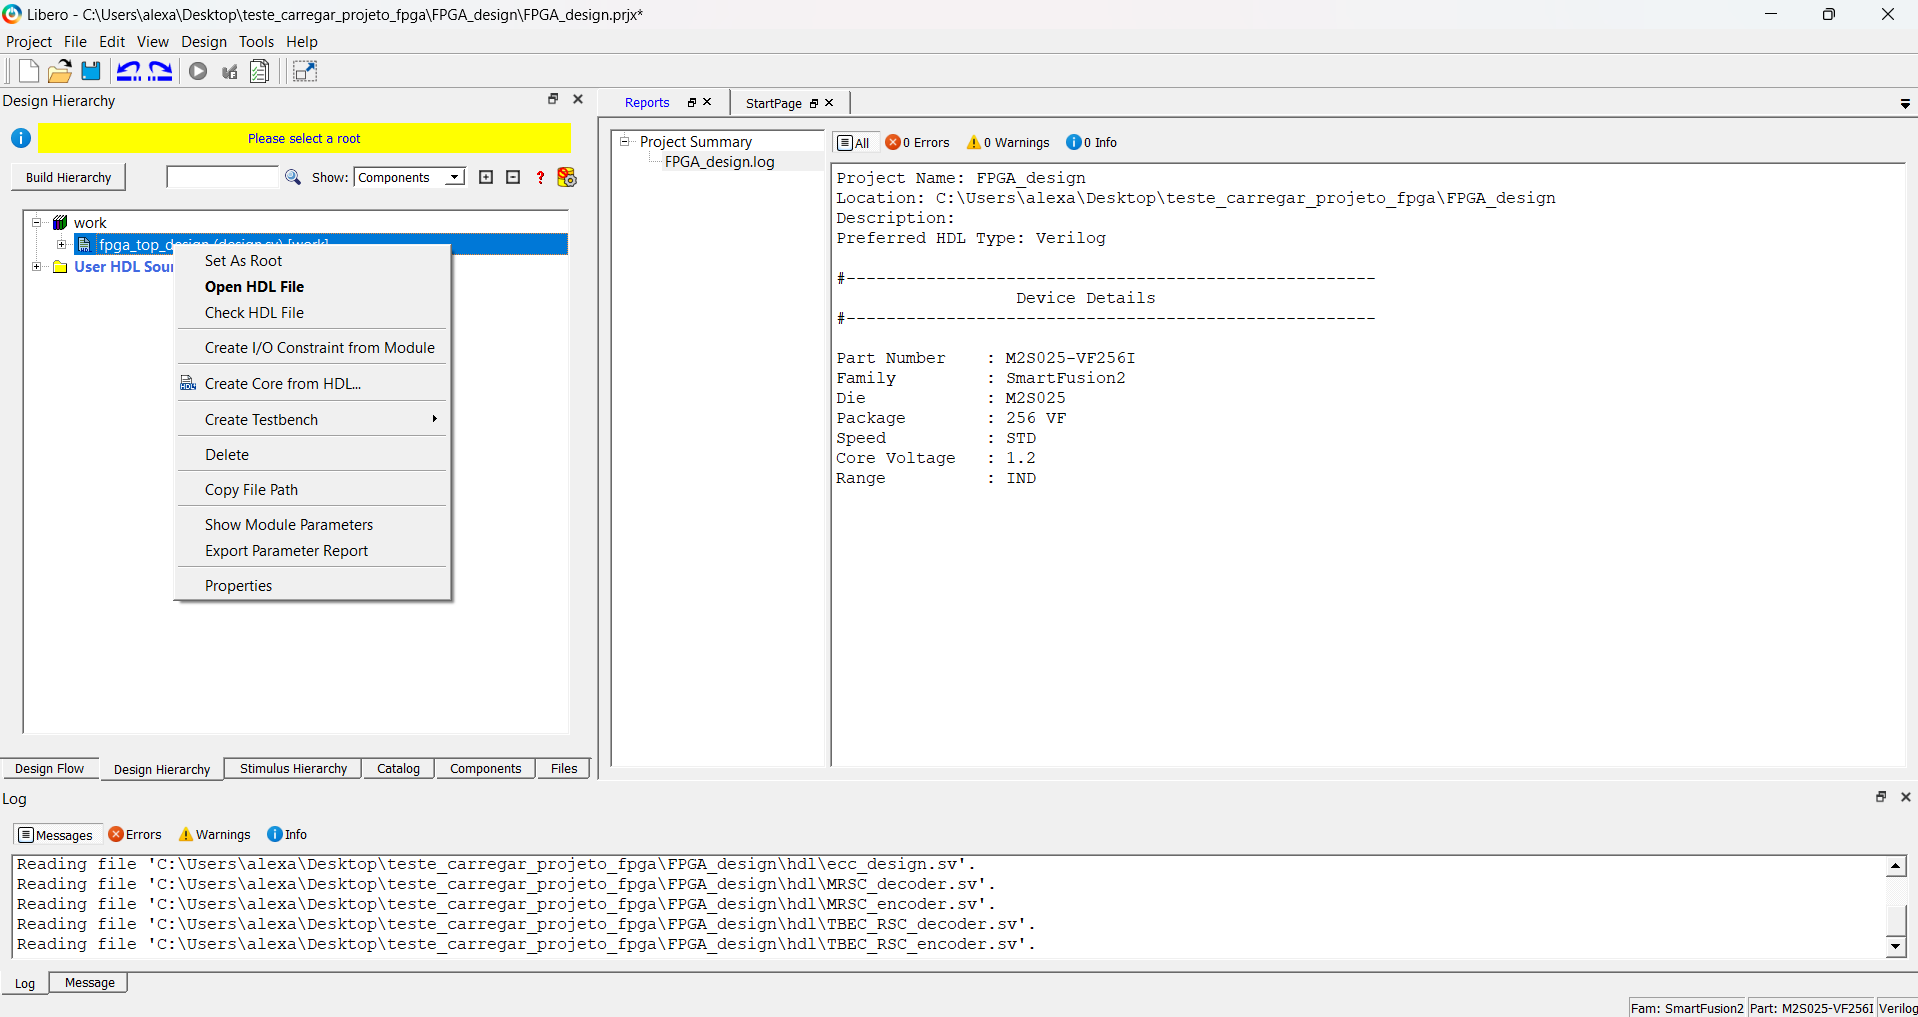
\includegraphics[width=0.85\textwidth]{tutorial_projeto_novo_libero_10.png}
    \caption{Menu de contexto do módulo \texttt{fpga\_top\_design}, com a opção \textbf{Set As Root} destacada.}
    \label{fig:novo_set_root}
\end{figure}

Uma vez definido o \textit{root}, o aviso amarelo desaparece e o painel
\textbf{Design Flow} passa a exibir \textbf{Top Module(root):
fpga\_top\_design} no topo da árvore de ferramentas, confirmando que o
projeto está pronto para prosseguir para a etapa de síntese (Figura
\ref{fig:novo_root_definido}).

\begin{figure}[h!]
    \centering
    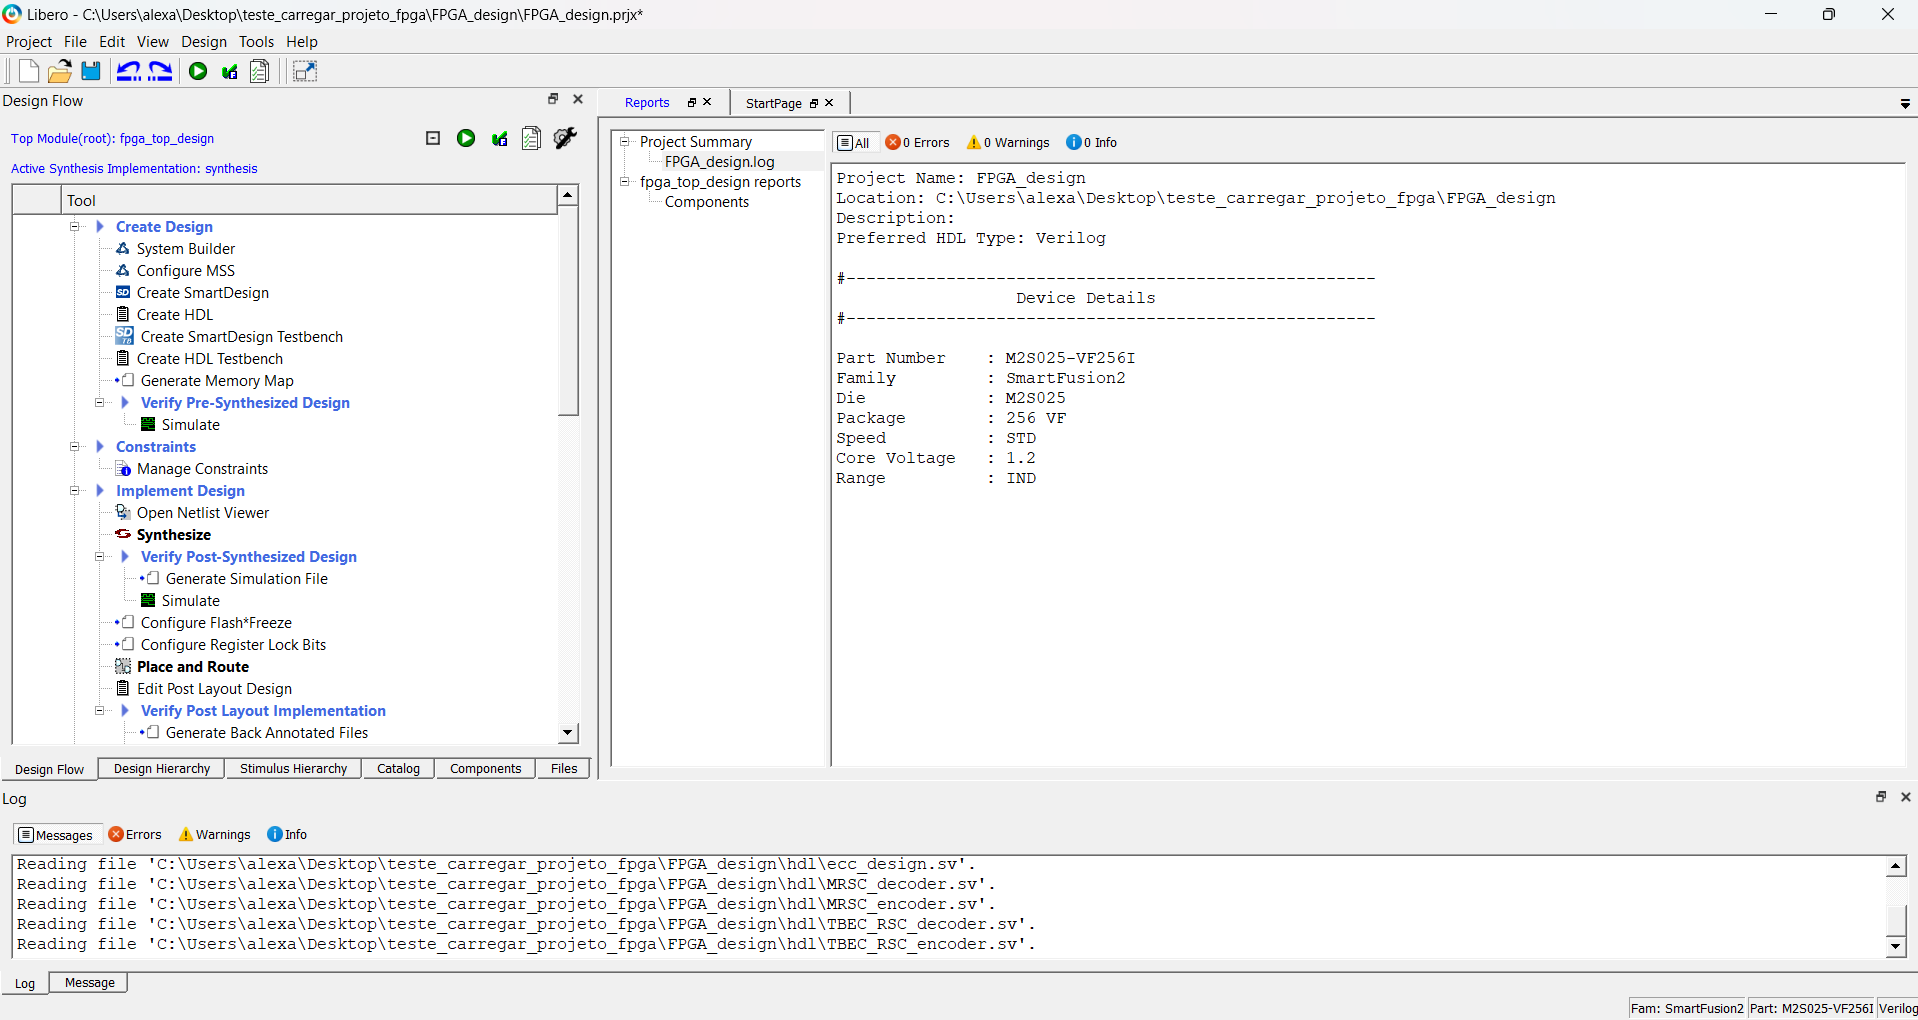
\includegraphics[width=0.85\textwidth]{tutorial_projeto_novo_libero_11.png}
    \caption{Painel \textit{Design Flow} após a definição do módulo de topo, exibindo \textit{Top Module(root): fpga\_top\_design}.}
    \label{fig:novo_root_definido}
\end{figure}

\subsubsection{Síntese Inicial e Verificação das Constraints}

Com o módulo de topo definido, executa-se a etapa \textbf{Synthesize}. O
painel de \textbf{Log} confirma a conclusão com a mensagem
\textit{"Synthesis completed"}. Em seguida, acessa-se o
\textbf{Constraint Manager}, na aba \textbf{I/O Attributes}, que neste
ponto do fluxo ainda se encontra vazia -- nenhuma constraint de pino foi
associada ao projeto até este momento (Figura
\ref{fig:novo_constraint_vazio}).

\begin{figure}[h!]
    \centering
    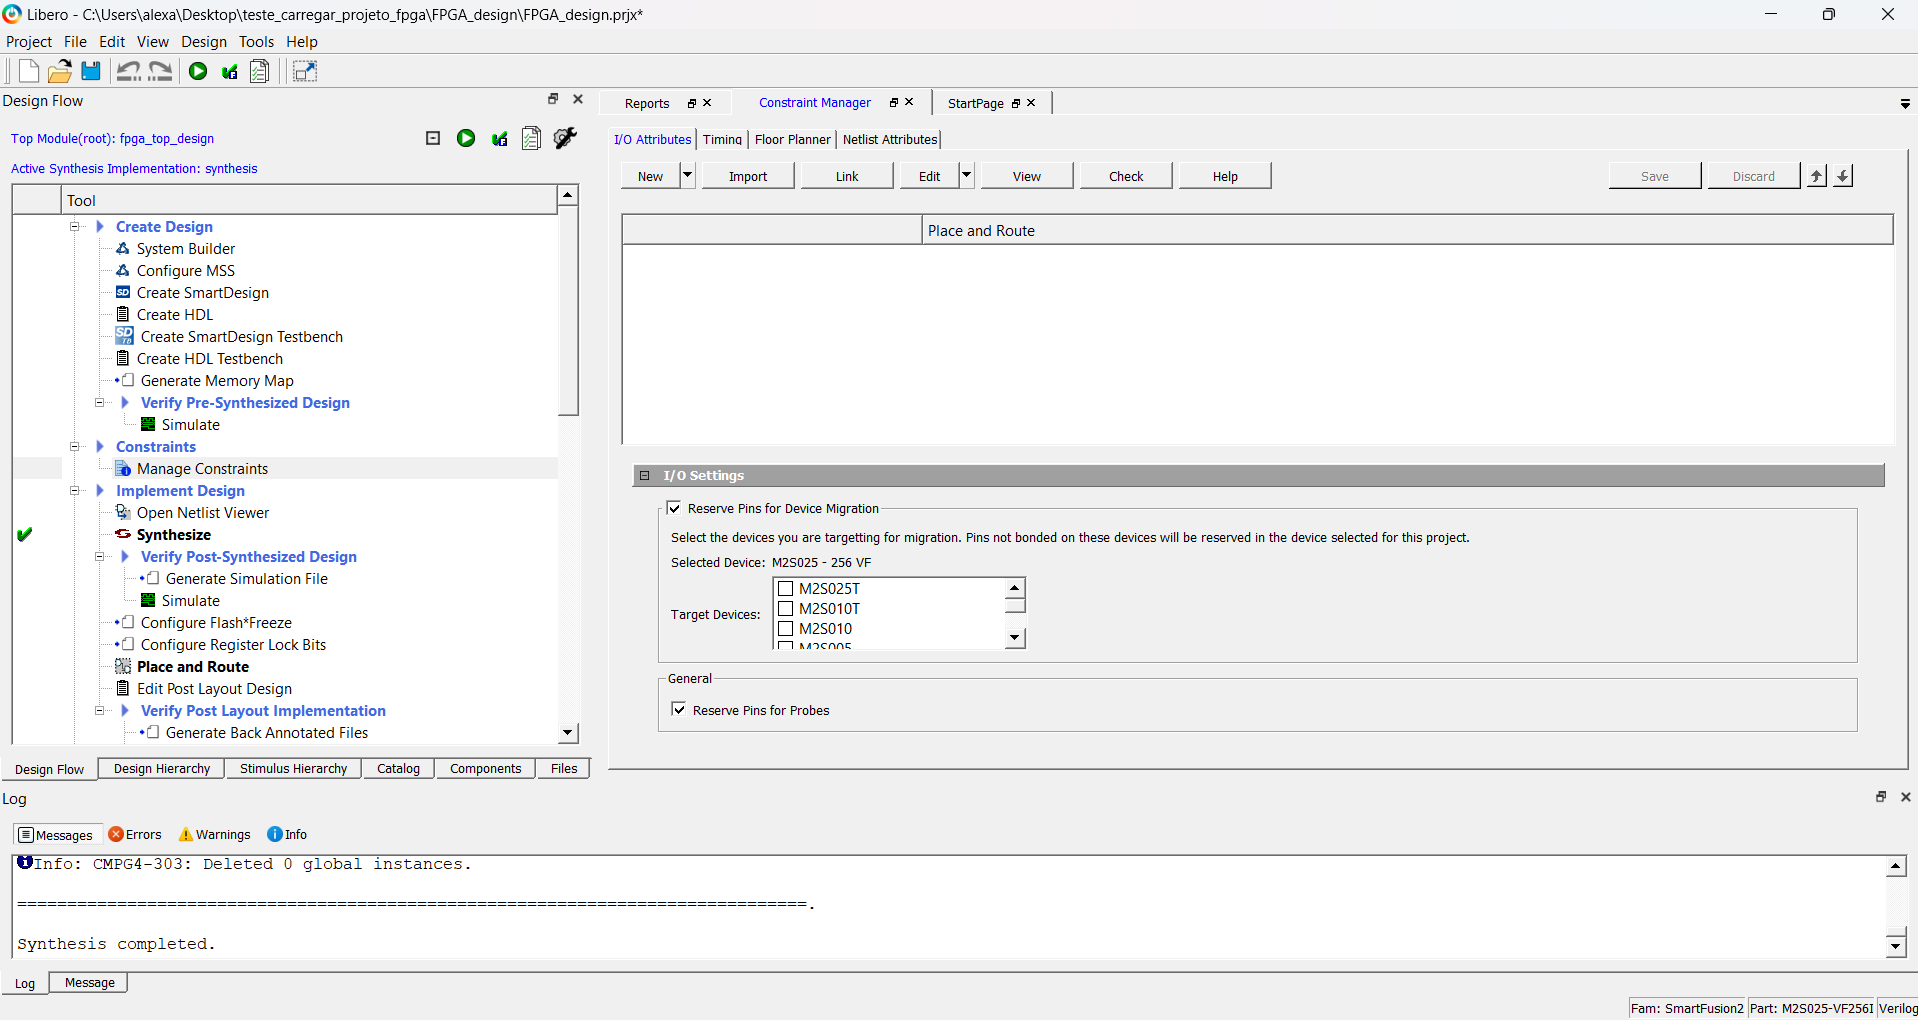
\includegraphics[width=0.85\textwidth]{tutorial_projeto_novo_libero_12.png}
    \caption{Aba \textit{I/O Attributes} do \textit{Constraint Manager}, ainda sem nenhuma constraint associada, logo após a conclusão da síntese.}
    \label{fig:novo_constraint_vazio}
\end{figure}

\subsubsection{Abertura do I/O Editor}

Para atribuir os pinos físicos às portas do módulo
\texttt{fpga\_top\_design}, clica-se na seta ao lado do botão
\textbf{Edit}, na barra de ferramentas do \textbf{Constraint Manager}, e
seleciona-se a opção \textbf{Edit with I/O Editor} (Figura
\ref{fig:novo_edit_io}), abrindo a ferramenta dedicada de edição de
pinos.

\begin{figure}[h!]
    \centering
    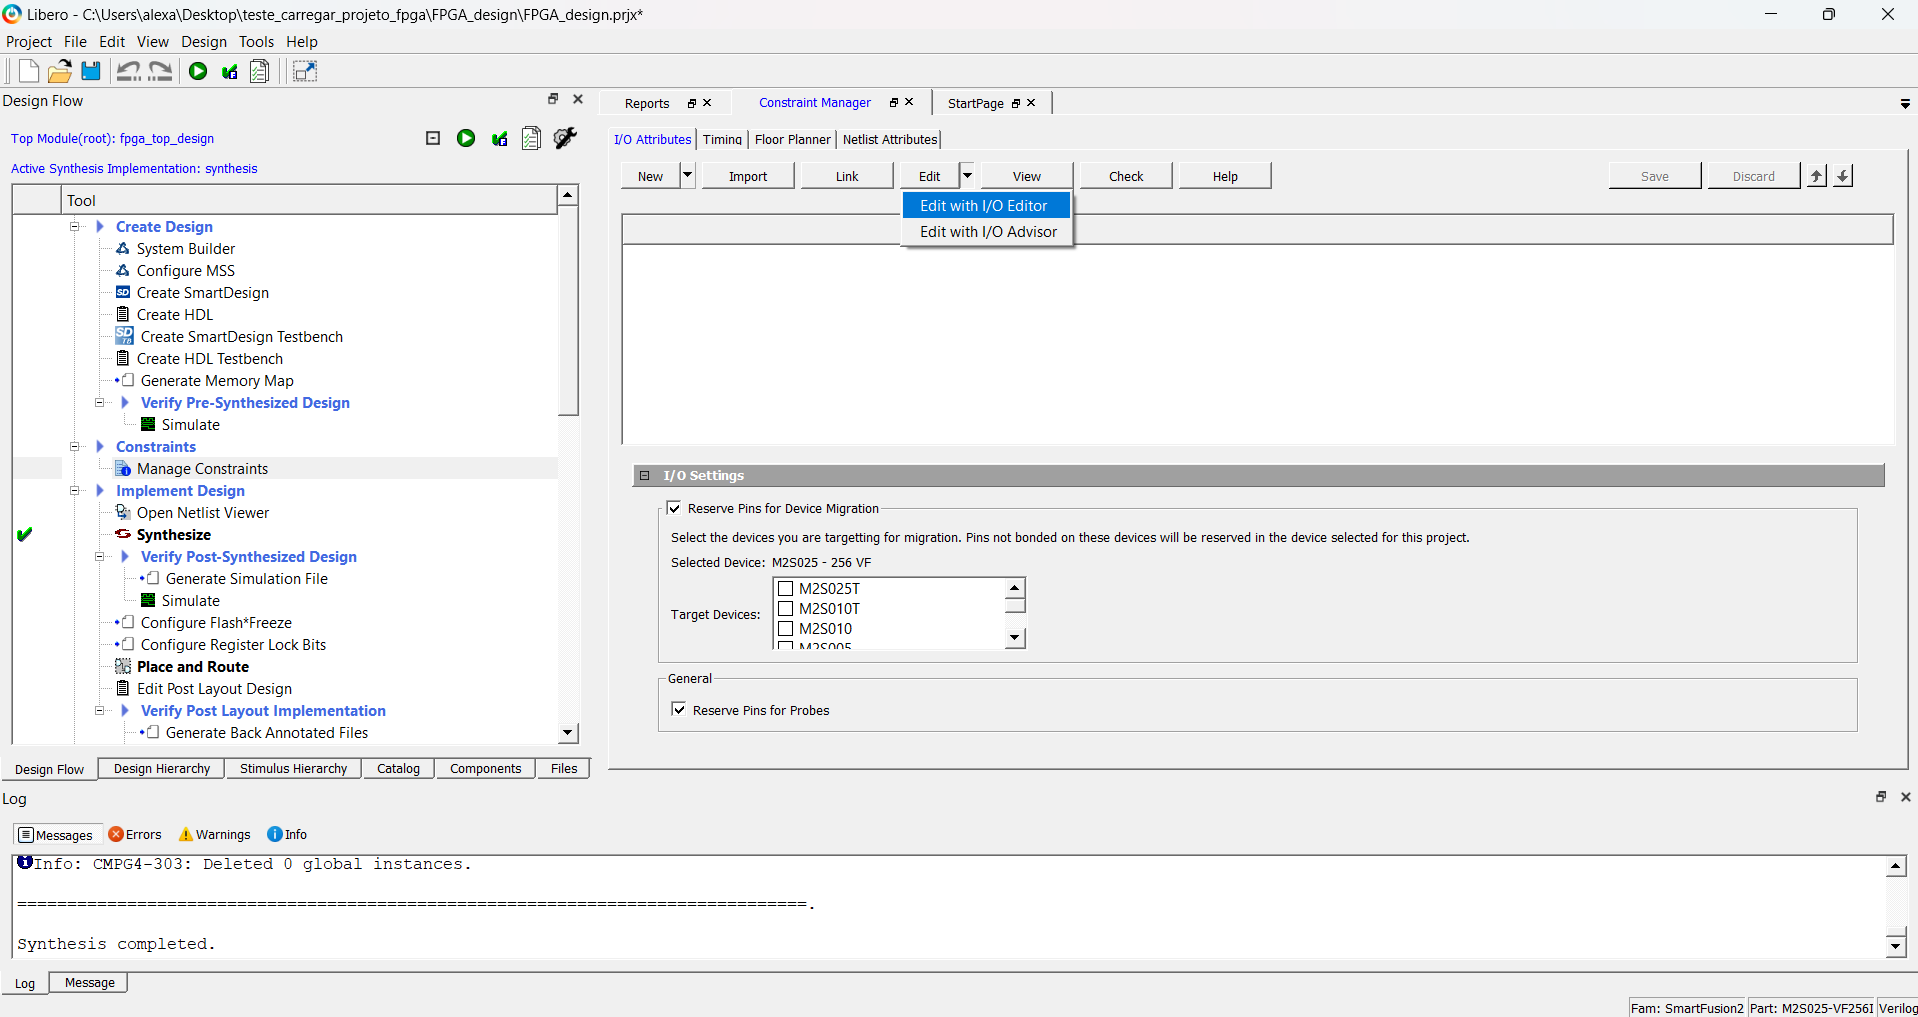
\includegraphics[width=0.85\textwidth]{tutorial_projeto_novo_libero_13.png}
    \caption{Menu do botão \textbf{Edit}, com a opção \textbf{Edit with I/O Editor} destacada.}
    \label{fig:novo_edit_io}
\end{figure}

\subsubsection{Atribuição dos Pinos no I/O Editor}

O \textbf{I/O Editor} exibe uma linha para cada porta do módulo
\texttt{fpga\_top\_design}, incluindo os barramentos expandidos bit a
bit (\texttt{ecc\_sel[0..2]}, \texttt{flag\_out[0..2]},
\texttt{chip\_sel\_out[0..1]}, \texttt{fpga\_mem\_io\_down[0..15]},
entre outros). Cada pino é atribuído digitando diretamente o número do
pacote na coluna \textbf{Pin Number} -- por exemplo, o pino \textbf{G16}
é atribuído à porta \texttt{ecc\_sel[0]} (Figura
\ref{fig:novo_io_editor_atribuindo}), reproduzindo o mapeamento de pinos
apresentado na Seção~\ref{sec:controle_perifericos}.

\begin{figure}[h!]
    \centering
    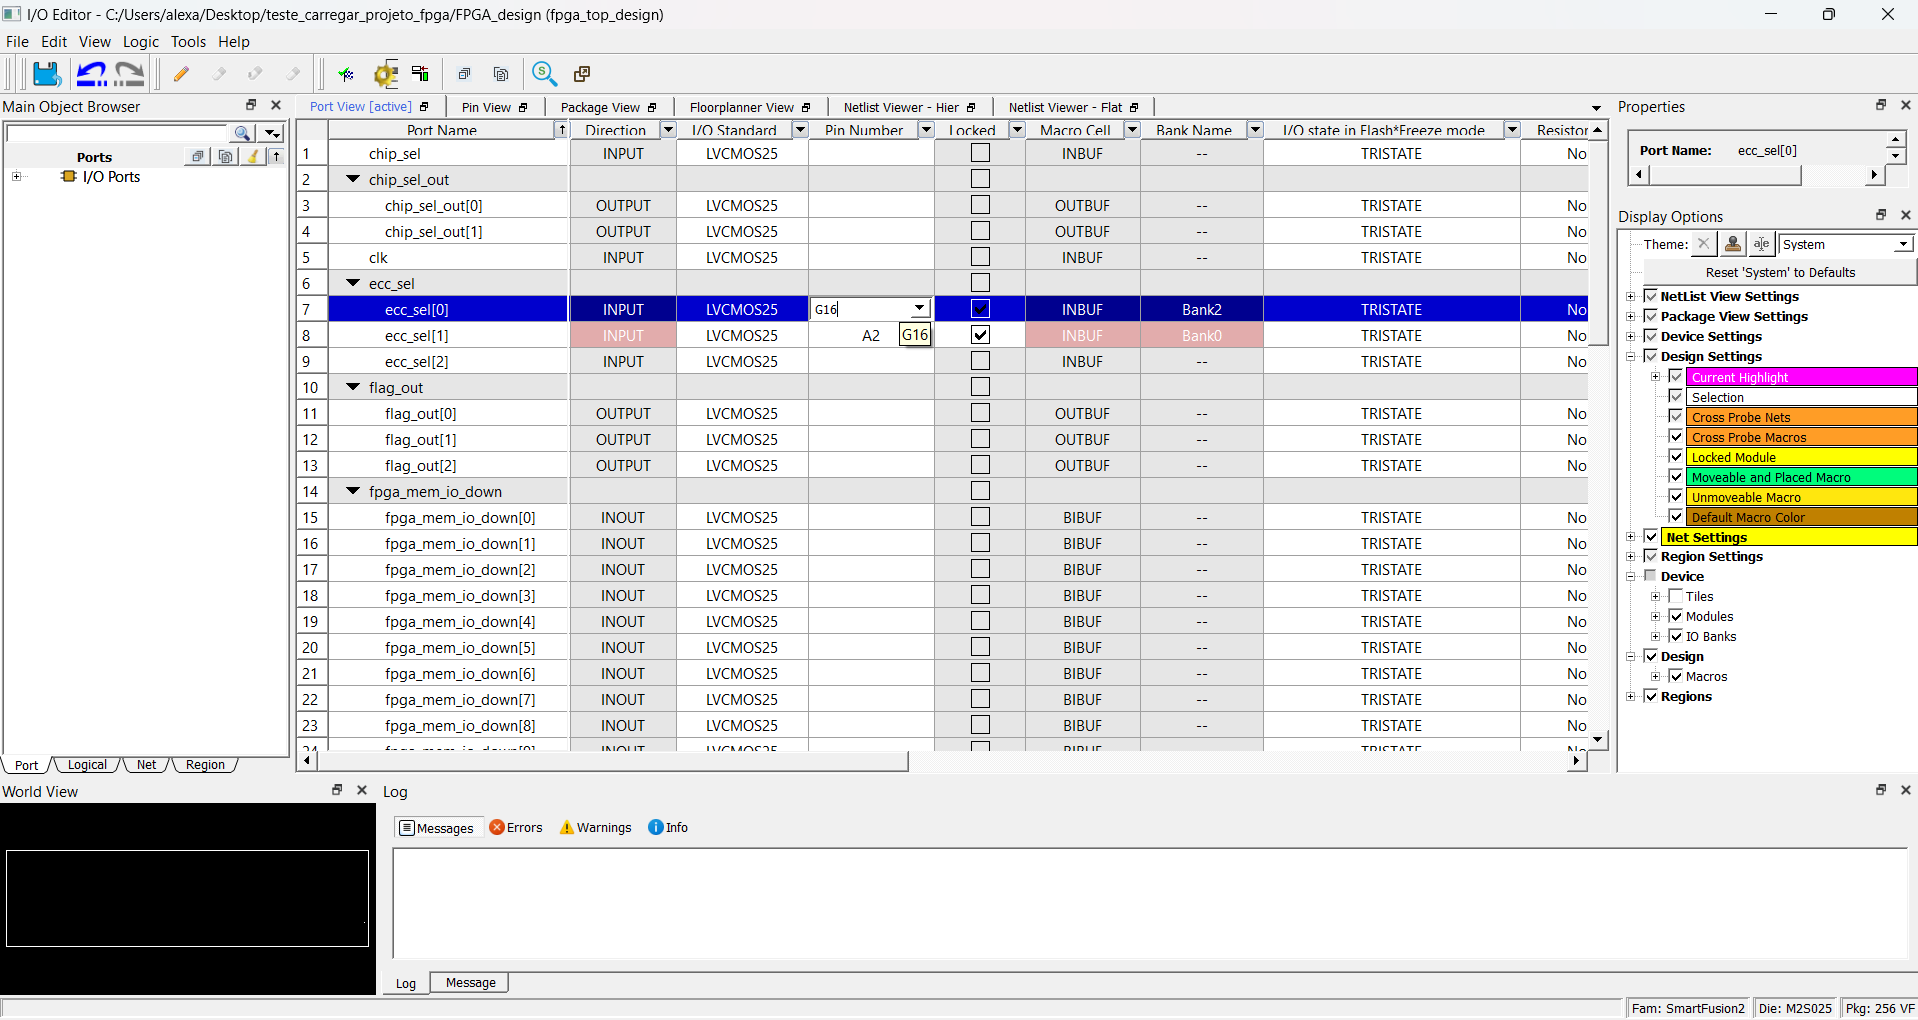
\includegraphics[width=0.85\textwidth]{tutorial_projeto_novo_libero_14.png}
    \caption{I/O Editor durante a atribuição do pino \textbf{G16} à porta \texttt{ecc\_sel[0]}.}
    \label{fig:novo_io_editor_atribuindo}
\end{figure}

Após a atribuição de todos os pinos e a marcação da coluna
\textbf{Locked} para fixá-los, executa-se o comando \textbf{Commit}.
Nesta etapa, o Libero valida cada valor digitado contra o pacote físico
selecionado, rejeitando pinos inexistentes ou incompatíveis -- as
mensagens \textit{"Pin Number can not be set to illegal value..."}
exibidas no painel \textbf{Message} (Figura \ref{fig:novo_io_editor_commit})
ilustram esse mecanismo de validação, indicando tentativas de atribuição
com identificadores de pino inválidos que precisam ser corrigidas antes
do \textit{commit} ser aceito para aquelas portas específicas. Ao final,
o Libero confirma a checagem das regras de projeto com a mensagem
\textit{"Design Rules Check completed successfully"} e grava as novas
constraints no arquivo
\texttt{constraint/io/user.pdc}.

\begin{figure}[h!]
    \centering
    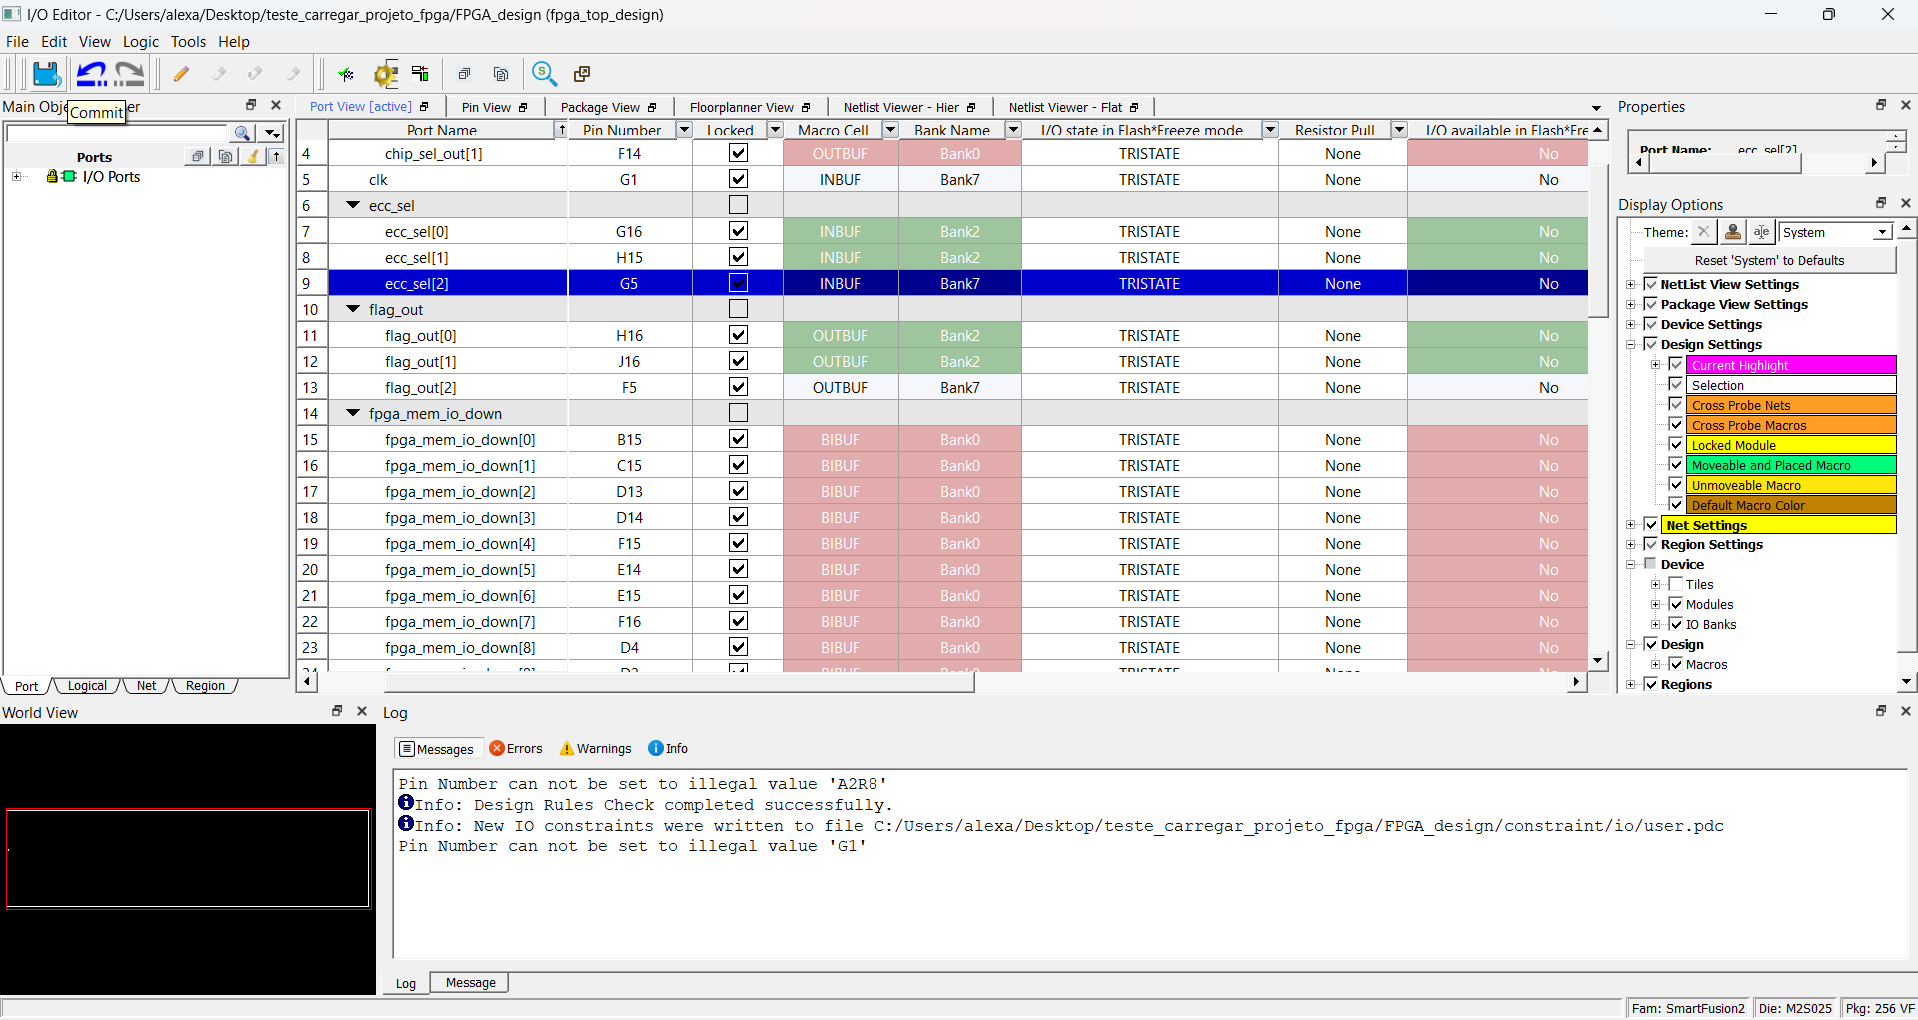
\includegraphics[width=0.85\textwidth]{tutorial_projeto_novo_libero_15.png}
    \caption{I/O Editor após o \textit{commit} dos pinos, com mensagens de validação exibidas no painel \textbf{Message}.}
    \label{fig:novo_io_editor_commit}
\end{figure}

\subsubsection{Continuação do Fluxo a partir do Place and Route}
\label{sec:tut_par_novo}

Com as constraints de pino corrigidas e comitadas com sucesso -- sem
nenhuma mensagem de erro remanescente --, o \textbf{Constraint Manager}
passa a exibir o arquivo \texttt{constraint\textbackslash io\textbackslash
user.pdc} associado como \textit{Target} da etapa \textbf{Place and
Route} (Figura \ref{fig:novo_pdc_alvo}), confirmando que o projeto está
pronto para prosseguir.

\begin{figure}[h!]
    \centering
    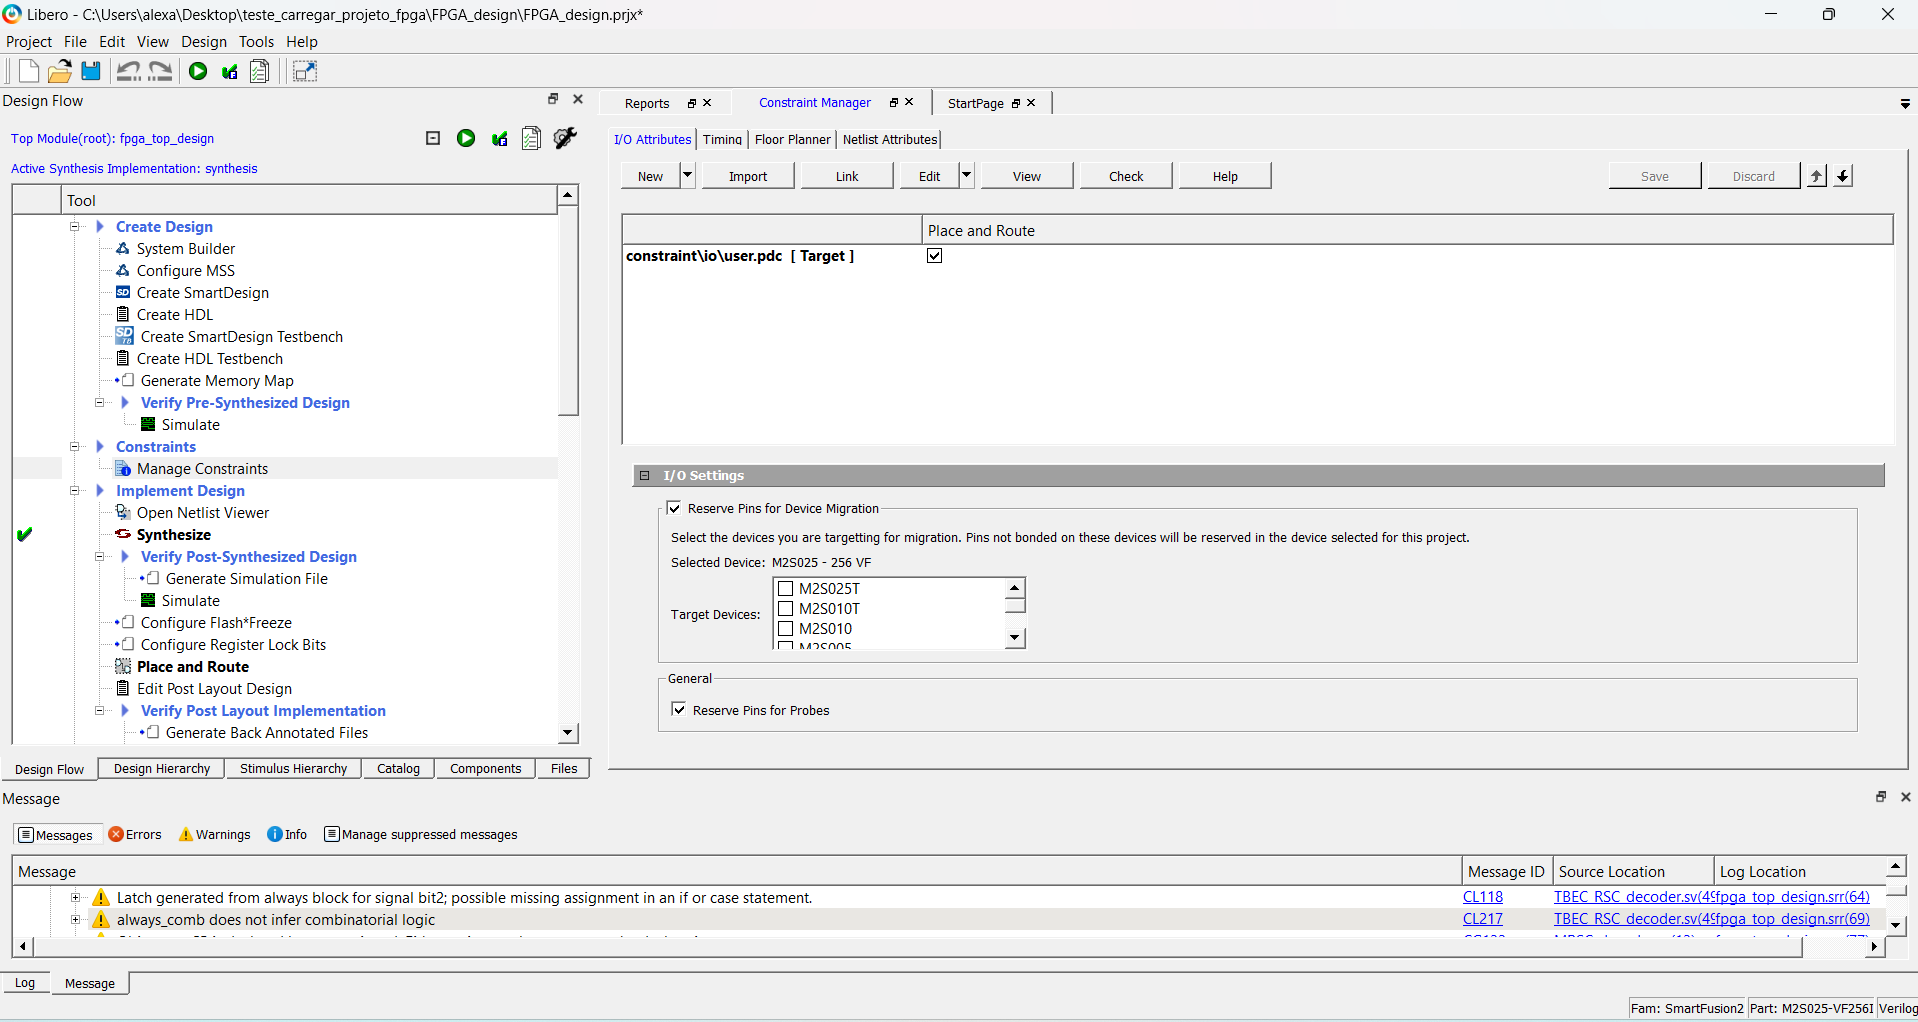
\includegraphics[width=0.85\textwidth]{tutorial_projeto_novo_libero_16.png}
    \caption{\textit{Constraint Manager} exibindo \texttt{user.pdc} associado como alvo (\textit{Target}) da etapa \textit{Place and Route}.}
    \label{fig:novo_pdc_alvo}
\end{figure}

\textbf{A partir deste ponto, o restante do fluxo de gravação é idêntico
ao já apresentado na Seção~\ref{sec:tutorial_libero}.} O leitor deve
prosseguir diretamente a partir da subseção \textbf{Place and Route},
executando em sequência: (i) \textit{Place and Route}
(Figura~\ref{fig:tut_par_report}); (ii) \textit{Generate Bitstream}
(Figura~\ref{fig:tut_bitstream}); (iii) \textit{Select Programmer}, com o
FlashPro5 conectado (Figura~\ref{fig:tut_select_prog}); e (iv)
\textit{Run PROGRAM Action}, concluindo a gravação do bitstream na FPGA
(Figura~\ref{fig:tut_program_done}), exatamente como descrito nas
Seções~\ref{sec:tutorial_libero} e seguintes.

\end{document}